%   
%\documentclass[12pt,a4paper]{memoir} % for a long document
\documentclass[12pt,a4paper]{memoir} % for a short document

\usepackage{amsmath}
\usepackage{graphicx}
\usepackage{color}   
%\usepackage[latin1]{inputenc}
\usepackage[utf8]{inputenc}
\usepackage[frenchb]{babel}
\chapterstyle{veelo}
% See the ``Memoir customise'' template for some common customisations
% Don't forget to read the Memoir manual: memman.pdf
\newlength{\drop}% for my convenience
\definecolor{Medium}{gray}{0.45}
 
\newcommand*{\titleJT}{\begingroup% Jan Tschichold: typographer
\drop = 0.08\textheight
\vspace*{\drop}
\hspace*{0.3\textwidth}
{\Large Dominique Aubert}\\[2\drop]
\hspace*{0.3\textwidth}{\Huge\itshape The Big Book of}\par
{\raggedleft\Huge\itshape Conundrums\par}
\vfill
\hspace*{0.3\textwidth}\\[0.5\baselineskip]  
\hspace*{0.3\textwidth}{\Large The Publisher}
\vspace*{\drop}
\endgroup}

\newcommand*{\titleTH}{\begingroup% T&H Typography
\raggedleft
\vspace*{\baselineskip}
{\Large Dominique Aubert}\\[0.167\textheight]
{\textcolor{Medium}{\Huge Cosmologie Physique}}\\[\baselineskip]
{\bfseries Une introduction}\\[\baselineskip]
{\small Master 2 spécialité astrophysique, Année 2015-2016}\par
\vfill
{\small Observatoire Astronomique de Strasbourg - Université de Strasbourg}\par
\vspace*{3\baselineskip}
\begin{figure}[htbp]
	\centering
		\includegraphics[height=10cm,width=12cm]{plots/homo/50mpc-1.jpg}
%	\caption{caption}
	\label{fig:plots_homo_50mpc-1}
\end{figure}
\endgroup}

\newcommand*{\titleGM}{\begingroup% Gentle Madness
\drop = 0.1\textheight
\vspace*{\baselineskip}
\vfill
\hbox{%
\hspace*{0.2\textwidth}%
\rule{1pt}{\textheight}
\hspace*{0.05\textwidth}%
\parbox[b]{0.75\textwidth}{
\vbox{%
\vspace{\drop}
{\noindent\HUGE\bfseries Some\\[0.5\baselineskip]
Conundrums}\\[2\baselineskip]
{\Large\itshape Puzzles for the Mind}\\[4\baselineskip]
{\Large THE AUTHOR}\par
\vspace{0.5\textheight}
{\noindent The Publisher}\\[\baselineskip]
}% end of vbox
}% end of parbox
}% end of hbox
\vfill
\null
\endgroup}

%%%%%%%%%%%%%%%%%%%%%%%%%%%%%%%%%%%%%%%%%%%%%
\newcommand{\ie}{\textit{i.e. }}
\newcommand{\md}{\mathrm{d}}
\newcommand{\cst}{\mathrm{cst}}
%%%%%%%%%%%%%%%%%%%%%%%%%%%%%%%%%%%%%%%%%%%%%


%%% BEGIN DOCUMENT
\begin{document}
\thispagestyle{empty}
\titleTH 


%\clearpage
%\include{foreword}  
\clearpage

\tableofcontents* % the asterisk means that the contents itself isn't put into the ToC

%!TEX root = /Users/domaubert/Documents/Lectures/cosmologie/cosmo_main.tex
\chapter{Etat des connaissances}

%\textit{Ce chapitre est tiré de \textbf{The Cosmological Parameters}, Lahav et Liddle, arxiv1401.1389}
%\newline
%\newline

L'objectif de ce chapitre est de faire un court panorama de l'état de nos connaissances sur les propriétés observées de l'Univers. Les chapitres suivant seront eux consacrés à l'élaboration des concepts et des théories qui permettent de rendre compte de ces propriétés observées. 

Concernant notre connaissance des propriétés de l'Univers, elle repose souvent sur \textit{l'interprétation d'observations au travers de théories et de modèles}. Par conséquent les propriétés décrites dans ce chapitre sont essentiellement valable dans le contexte du modèle standard de la cosmologie décrit dans les chapitres suivants. Si un changement de paradigme vient à opérer, rien n'empêche à priori que ces observations soit réinterprétées et donc conduise à modifier ce que nous savons de l'Univers.

\section{Observation fondamentale : le décalage vers le rouge}
L'observation première de la cosmologie, à l'origine même de l'émergence de la discipline au début du 20ème siècle, est la constatation que tous les objets observés à grande distance sont plus "rouges" qu'attendus. La mesure du spectre de ces objets indiquent que les systèmes de raies observés, parfois complexes, sont tous à des longueurs d'ondes plus importantes que ce que l'observation de ces mêmes éléments aurait donné dans un laboratoire. On définit le décalage vers le rouge ou "redshift" par la quantité z\index{redshift}
\begin{equation}
z\equiv\frac{\lambda-\lambda_0}{\lambda_0},
\end{equation}
où $\lambda$ est la longueur d'onde\index{longueur d'onde} observée et $\lambda_0$ celle mesurée en laboratoire. De plus ce rougissement est d'autant plus grand que la source est éloignée. 

Dans le cadre du modèle standard de la cosmologie, ce rougissement est de nature \textit{cosmologique} et traduit le phénomène \textit{d'expansion} de l'Univers. Dans ce processus d'expansion, toute distance prise entre 2 points de l'Univers est amené à évoluer \sidenote{en l'occurrence à augmenter dans un modèle standard d'Univers}. Notons dès à présent que cette augmentation n'est pas le symptôme d'un déplacement des sources par rapport à leur espace local mais plutôt la conséquence d'une dilatation de l'espace entre l'observateur et la source. Cette dilatation agit également sur la longueur d'onde des photons en vol et conduit au rougissement observé. Cette dilatation agit aussi sur les densités, diluant au cours du temps de telles quantités et on peut montrer qu'elle produit des dilatations des durées, on allongeant tout types d'intervalles temporels. Enfin, cette interprétation cosmologique permet également d'expliquer pourquoi ce décalage vers le rouge est d'autant plus important que la source est éloignée.

Notons que comme le redshift croît avec la distance, $z$ est de façon indirecte un indicateur de \textit{distance} et comme la lumière nous parvient avec une vitesse finie et connue, $z$ est également un indicateur de \textit{l'époque} à laquelle la source est observée. En cosmologie, l'action de désigner un objet ou un phénomène par son redshift $z$ implique à la fois une information spectrale, spatiale et temporelle.

Le processus d'expansion a débuté il y a 13.8 milliards d'années: c'est le \textit{Big Bang}\index{Big Bang}. Aux premiers instants, les distances étaient présumément courtes, l'Univers était donc de fait très dense. Régnait également une température très élevée, qui fut amenée à décroître au cours du temps\sidenote{Par exemple la température du 'gaz de photons cosmique', le fond diffus cosmologique, est aujourd'hui de 2.73 K mais était environ 1000 fois plus chaud lorsqu'il a été libéré. }. De fait le modèle accepté permettant de décrire les origines de l'Univers est parfois dénommé modèle du \textit{Big Bang chaud}.

\section{Propriétés générales de l'Univers}
L'Univers dans lequel nous vivons peut, semble-t-il, être décrit par une poignée de paramètres. La connaissance de ceux-ci, ajoutée à la connaissance de ce que nous croyons être les bonnes lois de la physique, permet d'expliquer une très grande partie des propriétés globales de l'Univers et également une grande partie des processus astrophysiques qui subissent la cosmologie qui les entoure.  

\subsection{Paramètres cosmologiques}
Comme détaillé dans les chapitres suivant, l'Univers peut être décrit à un haut niveau de précision en considérant qu'il est homogène, isotrope et possédant une dynamique régie par les équations de la relativité générale. Toutefois cette description nécessite la connaissance à priori de certains paramètres qui permettent d'expliquer l'Univers tel qu'il est observé. A l'inverse l'observation de l'état actuel du cosmos met des contraintes sur la valeur de ces paramètres.

\paragraph{Paramètre de Hubble} Le premier paramètre est le paramètre de Hubble $H_0$ \index{Hubble!paramètre}, qui caractérise le taux d'expansion actuel. Sa valeur est d'environ 70 km/s/Mpc. On utilise parfois le paramètre de Hubble réduit $h$ tel que $H_0=100 h$ km/s/Mpc~: sa valeur est proche $h\sim 0.7$.

\paragraph{Paramètres de densité} Les différents types d'énergie présents dans l'Univers ont une grande influence sur ses propriétés et leurs contribution au budget énergétique total est caractérisé par des paramètres de densité $\Omega_i$ \index{paramètre ! densité}. En pratique c'est le rapport de la densité d'énergie de type $i$ à une densité d'énergie de référence appelée \textit{densité critique\index{densité critique}}. On distingue la densité de matière $\Omega_m$, la densité de baryons (protons+neutrons(+électrons)) $\Omega_b$, la densité de rayonnement $\Omega_r$, la densité d'énergie des neutrinos $\Omega_\nu$ et la densité d'énergie noire\index{energie noire @énergie noire} $\Omega_\Lambda$. Il faut noter que la contribution de la matière contient celle des baryons\index{baryons}, par conséquent $\Omega_m\ge\Omega_b$: actuellement on a $\Omega_m\sim 0.3$ et $\Omega_b\sim 0.05$, la différence étant la contribution apportée par une matière \textit{non baryonique}, dite matière noire\index{matière noire}. Les contributions des espèces relativistes (photons, neutrinos) est aujourd'hui négligeable, bien que ce type de particule soit très abondant en nombre.

\paragraph{Spectre de fluctuations initiales} L'Univers tel qu'observé actuellement n'est pas strictement homogène, en particulier sur des échelles inférieures à la dizaine de Mpc. Les galaxies et amas qui nous entourent trouvent leur origine dans des fluctuations\index{fluctuations de densité} initiales de densité de très faible amplitude. Ces fluctuations sont caractérisées par un spectre  $P(k)$ qui donne la distribution des amplitudes des fluctuations de taille $L=2\pi/k$. On suppose actuellement que celles-ci trouvent leur origine dans la période \textit{d'inflation} qui prédit un spectre primordial de la forme \index{spectre ! puissance} :
\begin{equation}
P(k)\sim  k^{n_s},
\end{equation} 
$n_s$ constitue également un paramètre cosmologique et les modèles inflationnaire lui prédise une valeur \textit{proche mais différente} de \index{spectre ! inflation} l'unité \sidenote{le satellite Planck mesure ainsi une valeur proche de 0.96}. L'amplitude globale du spectre doit également être paramétrée, par exemple sous la forme d'une amplitude de fluctuation sur une échelle arbitraire de 8 Mpc, notée $\sigma_8$\index{spectre ! amplitude}. Notons enfin que les modèles d'inflations prédisent un fond d'ondes gravitationnelles\index{ondes gravitationnelles}, caractérisé par un spectre de fluctuations tensorielles, similaire à celui des fluctuations de densité (dites également scalaires). Le rapport d'amplitude entre fluctuations tensorielles et scalaires est noté $r$ et sa valeur est supposée quasi-nulle.

\paragraph{Etat d'ionisation de l'Univers} Le dernier paramètre canonique de la cosmologie permet de décrire l'état d'ionisation \index{ionisation} de l'Univers au cours de son histoire. Cet état se mesure en  contraignant le nombre moyen de diffusions des photons\index{photons} sur les électrons libres du cosmos\index{electrons@électrons}. Cette quantité est notée $\tau$ avec une valeur typique $\tau \sim 0.07$. L'essentiel de ces électrons libres sont produits au cours de la réionisation de l'Univers au redshift $z_\mathrm{reion}\sim 8$: dans les modèles les plus simples $\tau$ et $z_\mathrm{reion}$ sont directement liés.

\paragraph{Modèle minimal} L'ensemble des paramètres décrit précédemment permettent de rendre compte d'une grande variétés de propriétés observables. D'autre part, certaines hypothèses permettent encore de réduire le nombre de paramètres libres. Par exemple, l'inflation prédit une courbure\index{courbure} intrinsèque nulle qui se traduit en pratique par $\sum_i \Omega_i=1$. D'autre part l'amplitude des modes tensoriels (i.e. les ondes gravitationnelles issues de l'inflation) étant attendue comme très faible, on peut aisément poser $r=0$. Enfin, le paramètre de densité de rayonnement $\Omega_r$ est très précisément mesuré, par la mesure de température précise du fond diffus\index{fond diffus} ($T=2.7255\pm0.0006$ K) et ne permet donc plus de latitude significative sur sa valeur. Enfin , en l'absence de physique exotique la densité d'énergie des neutrinos $\Omega_\nu$ est directement liée à celle des photons \sidenote{tout en étant quasi nulle aujourd'hui}. Au final, un modèle extrêmement solide peut être construit avec seulement 6 paramètres libres. Au choix typique de "sextet" est $(\Omega_b,\Omega_m, H_0,\sigma_8,n_s,\tau)$. Bien sûr d'autres combinaisons de paramètres libres sont possibles.

\subsection{Principales sondes observationnelles}

Les paramètres précédents sont contraints par l'observation croisée de différentes sondes observationnelle. La convergence de ces valeurs conduit à ce qui est communément nommé \textit{le modèle de concordance}. Voici une liste (non-exhaustive) des principales sondes cosmologiques.

\paragraph{Mesure directe de $H_0$}
Cette mesure s'effectue à l'aide de chandelles standards qui permettent de mesurer indépendamment la distance d'un objet extra-galactique et son redshift $z$. La chandelle de référence est la relation période luminosité des étoiles variables de type Céphéides\index{Céphéides} la mesure de la période permet de déterminer la luminosité intrinsèque et donc la distance. Les Céphéides sont des indicateurs primaires et permettent de calibrer des indicateurs secondaires: courbes de lumières des supernovæ, relation de Tully-Fisher, etc... Ce type d'indicateurs donne une valeur de $H_0\sim 73$ km/s/Mpc. Le fond diffus cosmologique permet également une mesure indépendante de $H_0\sim 67$ km/s/Mpc en légère tension avec les estimateurs précédents.

\paragraph{Supernovæ et cosmologie}
La grande luminosité des supernovæ permet leur détection à des distances cosmologiques. De plus certains types de supernovæ\index{supernovae}, celles dite de type 'SN1A', ont un caractère quasi standard car elles résultent de l'explosion de naine blanche dans des systèmes binaires pour lesquelles il existe une forte corrélation entre luminosité et paramètres de la courbe de luminosité. L'accélération\index{accélération} \sidenote{c'est-à-dire le fait que les distances augmentent de plus en plus rapidement aujourd'hui} de l'expansion de l'Univers a été mise en évidence pour la première fois à l'aide de ce type d'indicateurs, en proposant pour la première fois la combinaison $\Omega_m=0.3$ et $\Omega_\Lambda=0.7$. De plus ces mêmes indicateurs indiquent que la densité d'énergie noire\index{energie noire@énergie noire} est une constante, donc équivalente à une constante cosmologique\index{constante cosmologique}\sidenote{on rencontrera aussi parfois le terme d'énergie du vide}.

\paragraph{Le fond diffus cosmologique}
Le fond diffus\index{fond diffus} cosmologique (Cosmic Microwave Background, CMB) est constitué des photons produits lors de la recombinaison\index{recombinaison}, 380 000 ans après le Big-Bang. Il constitue le plus grand réservoir de photons du cosmos et présente une brillance homogène à des niveaux de 1 pour 100 000. Le CMB présente néanmoins de faibles inhomogénéités qui tracent les inhomogénéités de matière à cette époque. La structure spatiale (en fait angulaire sur le ciel) comprend des informations sur toute l'histoire de croissance des structures depuis le Big-Bang jusqu'à 380 000 ans plus tard et sur les processus de couplage entre le rayonnement et la matière. L'étude de ces fluctuations permet par exemple d'établir la platitude de la géométrie de l'Univers, fournit une mesure de la quantité de baryons $\Omega_b$\index{baryons}, confirme la nécessité d'une matière non-baryonique et l'absence d'évolution de l'énergie noire. Le CMB indique également que le spectre de fluctuation initial est consistant avec les modèles d'inflation \index{inflation} et pour l'instant les modes tensoriels restent indétectables. Enfin le nombre de diffusion \index{diffusion} des photons sur les électrons est de l'ordre de $\tau\sim 0.07$ correspondant à une réionization vers un redshift de $z\sim8$. Le CMB constitue à l'heure actuelle la sonde la plus précise et la plus complète d'informations cosmologiques. C'est l'objet d'étude de missions spatiales et sol de très grande ampleur, dont par exemple le satellite européen \textit{Planck}.

\begin{figure}[htbp]
	\centering
		\includegraphics[height=10cm]{figs/pieplanck.png}
		\caption[Le bilan énergétique de l'Univers]{La répartition des différentes formes d'énergie au bilan énergétique total de l'Univers, d'après les mesures du satellite \textit{Planck}. On note l'absence de contribution du rayonnement et des neutrinos, dont le poids énergétique est trop faible pour pouvoir être représenté ici. La matière 'normale', désignée comme 'baryonique' et composée de protons, neutrons et électrons ne représente que $\sim 5\%$ du total. Le reste constitue le \textit{secteur sombre}.}
	\label{f:timeline}
\end{figure}


\paragraph{Grands relevés de Galaxies}
Les galaxies \index{galaxies} constituent des traceurs (biaisés) de la distribution de matière dans le cosmos. Par conséquent des efforts importants sont réalisés pour collecter de façon homogène, les positions dans le ciel et les propriétés de millions de galaxies, sous forme de grands relevés : parmi les plus connus on citera le \textit{Sloane Digital Sky Survey}, SDSS, ou bien le futur relevé fait du satellite européen \textit{Euclid}. En théorie, l'étude de la distribution spatiale de ces objets dans des grands relevés\index{grands relevés} doit permettre de contraindre le déroulé du processus de croissance des structures de l'Univers et par extension la cosmologie. Parmi les mesures les plus spectaculaires autorisées par ce type de relevés est la détection des oscillations baryoniques acoustiques\index{BAO} (BAOs) à bas redshift. Les BAOs sont déclenchés dans l'Univers pré-recombinaison et consistent en des ondes acoustiques dans le gaz baryonique entretenues par la compétition entre la pression de rayonnement et la gravitation produite par toute la matière. Ces BAOs sont gelés après la recombinaison\index{recombinaison} et se manifestent sur des échelles de 150 Mpc dans toute distribution de matière qui échantillonnent ces distances, dont le CMB et les grands relevés de galaxies.  La cosmologie issue des relevés de galaxies permet généralement de lever les dégénérescence entre paramètres, par exemple pour les estimations issues du CMB, et sont donc d'une importance essentielle. De plus les relevés opèrent à différents redshifts $z$ et offrent  des vues à différents instants d'une même sonde cosmologique (par exemple sur les BAOs) et sont donc des outils extrêmement puissants.

\paragraph{Amas de Galaxies}
Les amas de galaxies\index{galaxies ! amas} constituent les plus grands objets qui se sont effondrés gravitationnellement. Ils peuvent comprendre plusieurs milliers de galaxies et atteindre des masses allant jusqu'à $10^{15} M_\odot$. Le décompte de ces objets et leur fonction de masse permet ainsi de contraindre le champ de matière aux échelles qui viennent seulement de s'effondrer, sous l'action de la gravité\sidenote{on parle aussi de passage au régime non linéaire, en référence à la nature non linéaire des équations qui permettent de décrire ce processus}. On extrait de l'étude des amas généralement les quantités $\sigma_8\sim 0.8$ et $\Omega_m\sim0.3$. Ces amas sont généralement des émetteurs X, dont l'émissivité permet de déterminer la masse. On les détecte également dans le signal du CMB, comme des distorsions locales du spectre via l'effet Sunyaev Zeldovich\index{Effet SZ}.

\paragraph{Milieu Intergalactique}
La structure du gaz dans le milieu intergalactique\index{IGM} (IGM) nous renseigne également sur la distribution spatiale de la matière à différent redshift, via la mesure du spectre de puissance\index{spectre ! puissance} de la matière $P(k)$. La sonde la plus commune de l'IGM est la \textit{forêt Lyman-alpha}\index{forêt Lyman-$\alpha$}, qui se manifeste dans les spectres de quasars distants comme un ensemble de raies d'absorptions qui tracent la distribution de nuages absorbants le long de la ligne de visée. Dans le meilleur de cas, les BAOs\index{BAO} peuvent même être retrouvés (c'est le cas par exemple vers $z\sim2$) grâce à de multiples spectres pris le long de multiples directions vers des quasars\index{quasars} différents. Une autre application de l'étude de l'IGM pour la cosmologie consiste à observer les tunnels d'absorptions dans les spectres de quasars à très grand redshift $z>5.5$ : l'Univers y est jeune ($t<1$ Gyr) et encore neutre. La mesure de ces tunnels permet de contraindre l'histoire de réionisation\index{réionisation} de l'Univers et le paramètre cosmologique $\tau$.

\paragraph{Lentilles Gravitationnelles}
Les lentilles gravitationnelles\index{Lentilles gravitationnelles} traduisent la déformation de l'espace temps à proximité d'objets massifs, ce qui conduit également à une déformation de la trajectoire des rayons lumineux entre une source et un observateur. Dans les cas les plus spectaculaire (strong lensing) cela conduit à la production d'images multiples et à de fortes déformations de types arcs gravitationnels. Sur de grandes portions du ciel, le signal est beaucoup plus modéré bien que l'on s'attende à ce que par exemple le CMB ou bien la distribution de galaxies à un certain $z$ soient déformés par la distribution de matière entre eux et nous observateurs (weak lensing). Ces faibles déformations peuvent toutefois être analysées statistiquement pour conduire à des contraintes sur la distribution de la matière déformante $P(k)$ et à l'amplitude des fluctuations associées $\sigma_8$.

\section{Une Histoire du Cosmos}
\begin{figure}[htbp]
	\centering
		\includegraphics[height=10cm]{figs/timeline.png}
		\caption[Les grandes étapes dans l'histoire du cosmos]{Les grandes étapes dans l'histoire du cosmos. Cette frise couvre environ 13.8 milliards d'années d'évolution depuis le Big-Bang (à gauche) jusqu'à nos jours (à droite). \textit{Crédit:Planck-ESA}}
	\label{f:timeline}
\end{figure}

\newthought{Pour finir}, nous allons donner un cours descriptif des grandes étapes de l'histoire de l'Univers. Ces grandes étapes décrivent des processus physiques ou des transitions spécifiques qui opèrent à certains stades de l'évolution du cosmos et par extension sont aussi utilisés pour désignés des instants. Par exemple on parle de la réionisation pour désigner la fin du premier milliards d'années de l'Univers ou bien de l'inflation pour désigner ses premiers instants.

L'Univers a connu une phase extrêmement dense et chaude, il y a 13.8 milliards d'années. Nos théories actuelles ne nous permettent pas actuellement de remonter au delà d'un temps de Planck ($\sim 10^{-44}$ s), durée sur laquelle les effets de gravité quantique pourraient se manifester, mais à cette incertitude près, l'histoire de l'Univers débute à cette époque, nommée le \textit{Big-Bang}. A partir de cet instant, l'Univers va subir un effet d'expansion de l'espace et de baisse de sa température\index{température}. Dans le cadre du modèle cosmologique standard, les grandes étapes de son évolution sont les suivantes (cf. figure \ref{f:timeline}):
\begin{enumerate}
\item \underline{L'inflation} $t\sim 10^{-34}$ secondes\index{inflation} :  cette phase est encore spéculative et consisterait en une phase d'expansion accélérée de l'Univers dans ces instants quasi-initiaux. Si ce processus a bien eu lieu, il permettrait d'expliquer naturellement la grande homogénéité initiale de l'Univers, sa platitude et donnerait une origine quantique aux fluctuations initiales de matière qui sont à l'origine des grandes structures\index{grandes structures} actuelles de l'Univers. Ce processus aurait également été la source d'ondes gravitationnelles\index{ondes gravitationnelles} qui seraient toujours détectables et dont la découverte signerait la confirmation d'une phase d'inflation.
\item \underline{l'Univers primordial} $t<3$ minutes : au cours de cette époque l'Univers reste extrêmement chaud et dense. Il s'y déroule des processus à très haute énergie: plasma quark-gluons, confinement des quarks\index{quarks}, baryogénèse\index{baryogénèse} (i.e. l'annihilation matière anti-matière), découplage des neutrinos\index{neutrinos}, nucléosynthèse des éléments jusqu'à l'hélium\index{hélium}.
\item \underline{l'équivalence} $z=3400$ t=50 000 ans \index{equivalence@équivalence ! matière-rayonnement} l'Univers voit son bilan énergétique passer d'une domination par les espèces relativistes (le rayonnement) à une domination par la matière.
\item \underline{La recombinaison} $z=1100$ t=380 000 ans : l'Univers devient suffisamment froid (T=3000 K) et peu dense pour permettre la création d'atomes neutres et l'émission du fond diffus\index{fond diffus} cosmologique (CMB). 
\item \underline{les âges sombres} $1100>z>30$ \index{ages sombres@âges sombres} l'Univers est rempli de gaz froid et neutre. Le gaz se structure sous l'effet de la gravitation mais  n'est pas encore en mesure de former des étoiles\index{etoiles@étoiles}. 
\item \underline{la réionisation} $30>z>6$ le gaz parvient à des densité lui permettant de se convertir en étoiles. Ces étoiles vont émettre un rayonnement ionisant\index{ionisation} qui vont réioniser ($x_\mathrm{HI}\sim0.0001$) et réchauffer totalement l'Univers ($T\sim 10000$). C'est les stades initiaux de la formation des galaxies\index{galaxies}.
\item \underline{la formation des galaxies et des grandes structures} $30>z>0$ à partir de la formation des première étoiles vont se former les premières galaxies. Elles vont croître de façon hiérarchique \index{formation hiérarchique} par assemblage de petits objets pour former les plus gros, sous l'effet de processus d'instabilité gravitationnelle\index{instabilité gravitationnelle} dominés par une matière non baryonique. Les amas de galaxies\index{galaxies ! amas} vont apparaître vers $z=1$.
\item \underline{Accélération de l'expansion cosmique} $z\sim 0.3$, $t\sim 10$ milliards d'années. Le bilan énergétique de l'Univers devient dominé par l'énergie noire\index{energie noire @énergie noire}, induisant une expansion accélérée de l'Univers.
\item \underline{Aujourd'hui} $z=0$. L'Univers a 13.8 milliards d'années \index{age ! Univers}.
\end{enumerate}



%!TEX root = /Users/domaubert/Documents/Lectures/cosmologie/cosmo_main.tex

\chapter{Concepts Fondamentaux}

\section{Définition de l'Univers et de la Cosmologie}
\label{s:fond_def}
 On considère qu'il faut 3 constituants pour définir complètement un Univers:
\begin{enumerate}
\item un contenu en énergie, qui peut être sous diverses formes,
\item un jeu de lois physiques qui régit l'entrejeu des différentes énergies,
\item un espace-temps, qui est la scène sur laquelle cet entrejeu prend place.
\end{enumerate} 
L'enjeu de la \textit{cosmologie} est précisément d'étudier le contenu, les lois physiques et la structure de l'Univers. Par conséquent la cosmologie est liée aux aspects théoriques les plus fondamentaux de la physique mais également à des problèmes astrophysiques et il existe plusieurs manières de faire de la cosmologie. On cherchera par exemple à déterminer quelles sont les lois à l'œuvre dans le cosmos (point 2) , ce qui est davantage du domaine de la physique théorique, ou bien à déterminer les paramètres (point 3)  qui caractérisent la structure spatio-temporelle (e.g. sa forme ou bien son histoire) de l'Univers comme en cosmologie observationnelle. De même comprendre comment les différentes formes d'énergie (matière, lumière, etc...) s'organisent ou évoluent au cours du temps (point 1) (e.g. comment les grandes structures de l'Univers se mettent en place) permet d'avoir un éclairage sur les deux autres aspects du problème cosmologique.

\section{Principe Cosmologique}
L'objectif de la cosmologie est ambitieux et cette ambition n'est pas sans obstacles. L'un des problèmes les plus important est notre incapacité à garantir que ce que nous observons autour de nous reste valable à l'échelle du cosmos, \textit{y compris dans les régions de l'Univers qui nous serons à jamais inaccessibles}. Par exemple, rien ne garantit absolument que la neutralité électrique soit vraie dans tout le Cosmos ou bien que la densité de matière mesurée dans notre Univers observable soit effectivement celle de l'Univers entier. Aujourd'hui, il ne viendrait à l'idée de personne d'attribuer au cosmos une densité égale à celle de la Terre, pour autant c'est peu ou prou ce que nous faisons en cosmologie. 

Pour autant, \textit{nous n'avons pas le choix}. Par définition, il est impossible de connaître les propriétés de régions dont on ne peut extraire de l'information et toujours par définition, il existe de telles régions dans l'Univers. Quelle option reste-t-il à la personne désireuse de faire de la science à l'échelle de l'Univers, si ce n'est de supposer que ce qui nous est accessible est valide dans tout le cosmos ? En l'absence d'une telle hypothèse, il est tout simplement impossible de faire de la science avec l'Univers.

Cette supposition est à la base du \textit{Principe Cosmologique}. Si nous revenons sur les 3 constituants de la section \ref{s:fond_def}, il est aisé de reconnaître que cette supposition implique les contenu universel en énergie doit être le même que celui que nous constatons autour de nous. De même, la structure spatio-temporelle universelle doit être la même que celle que nous constatons dans l'Univers observable. Toutefois cette hypothèse "universaliste" implique également que nous supposons que les même lois de la nature s'appliquent dans tout le cosmos, y compris dans les régions qui nous sont inaccessibles ou pour lesquelles l'information n'est pas extractible. Le \textit{Principe Cosmologique} que nous retiendrons est le suivant : le contenu en énergie de l'Univers, sa structure spatio-temporelle et les lois qui y opèrent sont les même partout et par conséquent sont celles que nous constatons autour de nous. Notons tout de suite que cette universalité des composants s'applique aux échelles pertinentes pour la cosmologie et n'empêche pas des départs locaux aux valeurs universelles.

\subsection{Tautologie}

A ce stade, il nous semble que la cosmologie peut être définie par une tautologie~: \textit{la cosmologie est la science qui met le principe cosmologique à l'épreuve.} Si nous nous retrouvons dans une situation qui reste inexplicable dans ce que nous croyons être le jeu universel de contenu énergétique, spatio-temporel et "législatif" de l'Univers, alors les options sont réduites:
\begin{itemize}
\item soit nous continuons de croire que le principe cosmologique reste valide et c'est le détail de son contenu qui doit être révisé. Par exemple on modifiant les lois de la physique pour qu'elles rendent compte des nouveaux phénomènes tout en continuant à être une bonne description des processus locaux. C'est la voie scientifique standard.
\item soit nous renonçons au principe cosmologique et donc à l'universalité de ses composants et nous renonçons en même temps à l'ambition de décrire tout l'Univers avec la science que nous connaissons.
\end{itemize}

\subsection{Principe cosmologique pragmatique}
Le principe cosmologique est souvent décliné dans une version plus pragmatique qui est la suivante:
\begin{enumerate}
\item la gravitation est correctement décrite par la théorie de la relativité générale d'Einstein,
\item l'Univers est homogène et isotrope.
\end{enumerate}
Le point 2 revient à appliquer au cosmos ce que nous voyons de l'état de l'Univers autour de nous (contenu, géométrie, évolution etc...). Le point 1 revient à définir les lois universelles de la gravité~: une emphase particulière est mise sur cette interaction car elle est la seule qui \textit{in fine} est toujours de portée infinie et donc cosmologique. Par ailleurs, une fois la théorie de relativité générale choisie comme description correcte de la gravité, le point 2 a des conséquences que la relativité générale sait décrire dans le cadre d'étude qu'elle fixe.

\section{Relativité Générale: notions}
La gravitation est centrale à l'étude de la cosmologie car elle est la seule "force" dont l'action ne peut être écrantée et dont la portée soit infinie. De fait, elle est la seule force qui soit effective lorsque des échelles cosmologiques sont abordées. De plus la gravitation peut être décrite comme la manifestation des propriétés de l'espace-temps. Or il s'avère que la structure spatio-temporelle de l'Univers n'est pas triviale comme l'indique par exemple le phénomène d'expansion de l'Univers. Par conséquent l'observation de l'expansion du cosmos nous dit également des choses sur la façon dont la gravitation est à l'œuvre dans le cosmos. Compte tenu du rôle central de la gravitation pour les études cosmologiques, nous allons faire un aperçu de la théorie de la relativité générale et sur son application dans le cadre cosmologique

\subsection{Principe d'équivalence}
Le principe d'équivalence existe sous forme de différentes saveurs. La plus triviale est la suivante, où l'on considère le principe fondamental de la dynamique :
\begin{equation}
\frac{F_z}{m_i}=\ddot z.
\end{equation}
Ici l'on explique que l'accélération suivant la direction z est \textit{proportionnelle} à la force appliquée au système étudié et \textit{inversement proportionnelle} à un coefficient, que l'on nomme \textit{masse inertielle}. Par conséquent, deux systèmes soumis à la même force vont réagir différemment selon la valeur du coefficient $m_i$ qui les caractérisent. Intuitivement on comprend assez rapidement que ce coefficient est lié à la quantité de matière que le système possède, d'où sont qualificatif de masse~: un système fortement chargé en matière réagira moins qu'un système ayant une quantité de matière plus faible. Maintenant considérons l'expression de $F_z$ si cette force se trouve être une force de pesanteur~:
\begin{equation}
F_z=m_g g
\end{equation}
où g est la norme du champ de pesanteur. Cette force $F_z$ est d'autant plus forte que le coefficient $m_g$ est important~: ce coefficient caractérise également la quantité de matière dans le système et un système avec une grande quantité de masse va naturellement avoir une valeur élevée de $m_g$ et donc une pesanteur importante. Cette masse $m_g$ est aussi dénommée \textit{masse grave}.

A ce stade, nous avons donc deux coefficients qui tracent la quantité de matière dans un système physique:le premier $m_i$ lié aux équations de la dynamique, et sans aucune référence à priori à une force de pesanteur (ou de gravitation),  et le second $m_g$ qui lui pour le coup est complètement lié à la présence d'un champ de pesanteur. Il faut alors se rappeler qu'à priori, \textit{rien} ne nous informe d'une quelconque relation quantitative entre les deux et qu'il faut postuler une éventuelle relation entre les masses inertielles et graves.

Toutefois, l'expérience nous indique que tous les systèmes soumis à un champ de pesanteur donné semblent posséder la même accélération $\ddot z$ et ceci quelles que soient leur masse inertielle et grave. Ceci implique que $m_g\sim m_i$. Plutôt qu'une vague égalité, \textit{le principe d'équivalence} stipule une exacte identité entre ces deux quantités:
\begin{equation}
m_g=m_i.
\end{equation}
Cette égalité est fortement suggérée par l'expérience, mais ne peut être démontrée être absolument valide. Selon ce principe, la quantité de matière intervient au travers d'une valeur unique qui est \textit{la masse} $m=m_g=m_i$. On peut noter dès à présent que cette égalité confère à la gravitation un rôle spécial~: la masse \textit{inertielle} est lié à la loi décrivant la dynamique des systèmes, y compris en l'absence de gravitation. Par exemple, une particule chargée dans un champ électrique verra son accélération modulée en $q/m_i$. La force électrostatique, comme toutes les autres forces subit l'impact de ce coefficient d'origine dynamique. D'après le principe d'équivalence, la gravitation quant à elle possède \textit{dans sa propre expression} ce même coefficient, avant expression d'un quelconque problème dynamique. Elle dispose donc d'une façon innée d'une sorte d'élément d'information sur la façon dont la dynamique est régie, information que ne possède pas les autres interactions.

\subsection{Référentiel inertiel}
L'équivalence entre masse grave et inertielle a plusieurs conséquences. Comme déjà mentionné, elle permet de rendre compte de l'universalité de l'accélération de systèmes différents dans un même champ de pesanteur. C'est la fameuse expérience de la tour de Pise où des masses différentes parviennent au sol au même instant car étant accélérée exactement de la même façon. Il en découle également que si l'on fait le choix d'étudier la chute libre de plusieurs objets dans un référentiel lui même en chute libre, ces objets apparaissent tous comme en "flottaison" comme si l'on avait annulé la gravitation dans ce référentiel et ceci même si ils sont tous très différents. A nouveau cela n'est possible que parce que la chute libre dans un champ de pesanteur est la même quel que soit l'objet considéré. Ce type de référentiel est appelé \textit{référentiel inertiel}. Généralement un tel référentiel ne peut être construit que localement et par exemple dans un champ de pesanteur radial, il est possible de construire une collection de référentiel inertiels qui annuleront la gravité localement mais aucun de ces référentiels ne peut annuler globalement le champ de pesanteur. A ce titre il est usuel de se référer à ce type de référentiel sous l'appellation \textit{référentiel localement inertiel}. Cette possibilité d'annuler localement la gravité est intrinsèquement lié à l'égalité $m_i=m_g$. Ce lien est si fort que l'on va considérer que \textit{la possibilité d'annuler la gravitation par un choix approprié de référentiel est aussi un énoncé du principe d'équivalence}. 

Notez qu'à l'aide d'un choix approprié de référentiel on peut également créer de la gravité. Si des systèmes libres sont placés dans un référentiel uniformément accéléré, ils percevront leur mouvement relatif comme induit par une force de gravitation. \textit{De façon générale il est impossible localement de distinguer un référentiel uniformément accéléré d'un champ de gravitation.}

\subsection{Qu'est-ce que la gravitation ?}
A nouveau, on peut créer ou "détruire" un champ gravitationnel par un choix approprié de référentiel. Or un référentiel pourrait se résumer à un ensemble de règles et d'horloges ayant un certain comportement donc à un objet qui n'a qu'une nature géométrique et non pas physique. A partir de cette constatation, il est tentant de considérer alors que la gravitation n'est qu'une manifestation géométrique de l'espace dans lequel évoluent les systèmes. C'est le choix que fait la théorie de la relativité générale (RG par la suite), où la gravitation n'est pas une force à proprement parler mais davantage une manifestation de la géométrie de l'espace-temps. En RG, les systèmes se déplacent librement dans une géométrie qui, si elle est non triviale, produit des effets qui peuvent être interprétés comme le produit d'une interaction. A ce titre on peut dire que \textit{la gravitation n'existe pas}, elle n'est qu'une interprétation d'un effet de nature fondamentalement géométrique. 

Ainsi, on verra par la suite que c'est la courbure de cette géométrie qui produit les effets gravitationnels. A l'inverse, une géométrie sans courbure, i.e. une géométrie plane, produit un environnement sans effets de gravitation. Or il est aisé d'imaginer qu'il est toujours possible de trouver \textit{localement} un jeu de coordonnées qui rendent une géométrie plane, i.e. une transformation \textit{locale} qui permette de détruire la gravitation. Par analogie, une fonction régulière peut être approximée comme une collection de tangentes sur lesquelles il n'y a pas de courbures et qui localement sont des représentations exactes de la fonction originale. C'est une manifestation du principe d'équivalence~:\textit{il est toujours possible de trouver une transformation locale qui rende la géométrie de l'espace-temps plane}. Plus précisément c'est parce que l'on considère la gravitation comme étant de la géométrie que le principe d'équivalence se trouve naturellement réalisé.

Cette vue de la gravité comme géométrie de l'espace-temps est l'école classique d'interprétation de la RG. Elle n'est toutefois pas sans poser problème par exemple si l'on cherche à quantifier la gravitation. Si cette dernière est pure géométrie alors on peut arguer qu'il n'y a rien à quantifier et par exemple il n'y a pas de raison à priori d'invoquer l'existence d'un boson porteur de l'interaction, coupant court à toute tentative de quantification et donc d'unification. Si l'on estime que la quantification est nécessaire alors la vision géométrique n'est qu'une interprétation, certes très puissante, d'un processus qui n'est pas pure géométrie. Dans ce cadre le principe d'équivalence devient prééminent: il faut le supposer réalisé par un mécanisme encore inconnu et sa réalisation conduit à une possible interprétation géométrique. L'approche classique vue précédemment raisonne de façon inverse.

\subsection{Espace-temps et Métrique}
La théorie de la relativité générale décrit la gravitation comme une manifestation de la géométrie de l'espace-temps. Cet espace temps possède 4 dimensions, une de temps et trois d'espace. L'outil mathématique permettant de décrire cette géométrie est la géométrie différentielle. Une quantité centrale est \textit{la métrique}~: fondamentalement elle est l'outil qui permet de calculer des distances (des produits scalaires) dans une géométrie arbitraire. En notation d'Einstein, le calcul d'une distance s'écrit de la façon suivante :
\begin{equation}
ds^2=g_{\mu\nu}dx^\mu dx^\nu,
\label{e:scal}
\end{equation}
où les indices $\mu,\nu$ courent sur les indices des coordonnées, $ds^2$ est un scalaire donnant la distance couverte par un intervalle $(dx^0,dx^1,dx^2,dx^3)$. La quantité $g_{\mu,\nu}$ est la métrique et permet de relier la distance aux composantes de l'intervalle. Si la géométrie est plane, la métrique aura une certaine forme et si la géométrie est courbe et complexe, cette expression sera différente. En géométrie euclidienne plane à 3D le calcul de distance est le suivant:
\begin{equation}
ds^2=(dx^1)^2+(dx^2)^2+(dx^3)^2.
\end{equation} 
En géométrie de Minkowski, correspondant à l'espace-temps plat utilisé par la relativité restreinte, le calcul devient
\begin{equation}
ds^2=(dx^0)^2 -((dx^1)^2+(dx^2)^2+(dx^3)^2)
\end{equation} 
où $dx^0=cdt$ est la composante liée au temps. L'expression générale est elle donnée par Eq. \ref{e:scal}.

Cette métrique synthétise la structure spatio-temporelle de la \textit{variété} que l'on cherche à étudier. Pour faire de la cosmologie, il faut ainsi se doter d'une telle métrique, la plus à même de représenter ce que l'on croit être les caractéristique générique du cosmos.

\subsection{Métrique de Friedman-Robertson-Walker}
En se rappelant l'énoncé du principe cosmologique pragmatique, la métrique devant servir à décrire l'Univers doit refléter les propriétés d'homogénéité et d'isotropie. La métrique la plus générique satisfaisant ces contraintes est la métrique de Friedman-Robertson-Walker (FRW). A l'aide de celle-ci, l'intervalle de distance 4D est donné par:
\begin{equation}
ds^2=c^2dt^2-a(t)^2(\frac{dr_0^2}{1-Kr_0^2}+r_0^2d\theta^2+r_0^2\sin^2\theta d\phi^2).
\label{e:FRW}
\end{equation}
On note que cette métrique fait usage d'un système de coordonnées sphériques $(r_0,\theta,\phi)$ pour sa partie espace. On note également que par rapport aux exemples Euclidien et Minkowskien, FRW couple explicitement les parties temporelles et spatiales, via le facteur d'expansion $a(t)$.  

$r_0$ est une \textit{distance comobile}~: c'est une coordonnée de nature spatiale et indépendante du temps. Ici elle désigne une distance radiale prise à partir de l'origine du système de coordonnées et est également prise en compte pour calculer les contributions à l'intervalle des séparations angulaires $d\theta$ et $d\phi$. Le paramètre $K$ est un paramètre \textit{de courbure} auquel on peut éventuellement associer un rayon de courbure $R_K=K^{-1/2}$.

Si l'on considère deux évènements sur une même ligne de visée (donc avec $d\theta=d\phi=0$), l'intervalle peut se synthétiser sous une forme
\begin{equation}
ds^2=c^2dt^2-dr^2,
\end{equation}
avec 
\begin{equation}
dr=\frac{a(t)dr_0}{\sqrt{1-Kr_0^2}}.
\label{e:phydist}
\end{equation}
Ici $dr$ désigne la distance \textit{physique} de la partie spatiale (donc 3D) de l'intervalle que nous étudions. Cette distance dépend du temps, donc de l'instant considéré, et est modulé par une éventuelle courbure. A proximité de l'origine ($r_0\rightarrow 0$) ou dans des régimes de très faible courbure ($R_K\rightarrow\infty$ ou $K\rightarrow 0$), distance physique et distance comobile sont directement reliées par :
\begin{equation}
dr=a(t)dr_0.
\end{equation}
Là où la distance comobile était une quantité statique, la distance physique est une quantité évolutive, dont la dépendance temporelle est encodée par le facteur d'expansion $a(t)$. Notons que si l'on considère le parcours d'un photon sur un intervalle infinitésimal ($t$ est alors quasi constant et $r_0<<1$) alors $dr=cdt$ et la distance physique est celle effectivement parcourue par le rayon lumineux. Si la géométrie est plane, $K=0$, et la distance de parcours lumineux \textit{dans ce cas précis} vaut $D_L=dr=a(t)dr_0$.  Si toutefois la courbure de l'espace est positive et non nulle, alors $ D_L>a(t)dr_0$ et dans le cas d'une courbure négative $ D_L<a(t)dr_0$~: de façon générale, la courbure induit un départ de la distance physique par rapport à une fonction simple de la distance comobile.

Considérons à nouveau la distance physique en se plaçant à un instant donné et en calculant $r(t)$ entre 2 points A et B, séparés d'une distance comobile $R_0$ le long d'une direction avec $(\theta,\phi)$ donnés. En pratique il s'agit d'intégrer l'équation \ref{e:phydist} tout en considérant $t$ constant. On a alors
\begin{eqnarray}
&&a(t)R_0\\
r(t)&=&a(t)R_K \arcsin(R_0/R_K)\\
&&a(t)R_K \mathrm{argsh}(R_0/R_K)
\end{eqnarray}
pour une courbure $R_K=K/|K|^{3/2}$ respectivement nulle, positive et négative. Notons que les termes de courbure sont indépendants du temps. Les trois solutions peuvent être synthétisées sous la forme d'une équation unique $r(t)=a(t)S_K(r_0)$. A nouveau, les distances physiques sont des fonctions du temps qui ne dépendent que de la variation temporelle du facteur d'expansion $a(t)$. Si $a$ est un fonction croissante, \textit{toutes} les distances augmentent avec le temps et on parle d'Univers en expansion. A l'inverse, $a$ peut être une fonction décroissante du temps, auquel cas l'Univers est en contraction.

Pour finir, mentionnons que les distances physiques aujourd'hui sont obtenues en prenant la valeur du facteur d'expansion prise aujourd'hui. Ces types de quantités mesurées aujourd'hui sont notées par convention avec l'indice 0. Par exemple le temps qui a pu s'écouler depuis le Big-Bang jusqu'à aujourd'hui est noté $t_0$. De même le facteur d'expansion aujourd 'hui est noté $a_0=a(t_0)$.
\textit{Par convention} le facteur d'expansion est normalisé à cette valeur actuelle et 
\begin{equation}
a_0=a(t_0)=1.
\end{equation}
Il en découle que 
\begin{equation}
r(t_0)=S_K(r_0).
\end{equation}
et dans le cas sans courbure, on constate que la distance physique mesurée aujourd'hui est égale à la distance comobile $r(t_0)=r_0$.

\subsection{Facteur d'expansion, Loi de Hubble}
La distance physique $r(t)$ entre deux points peut être simplement dérivée au cours du temps.
\begin{equation}
\dot r(t)= \dot a S_K(r_0) =\frac{\dot a}{a}r(t).
\end{equation}
On définit le \textit{paramètre de Hubble} comme la fonction dépendante du temps donnée par :
\begin{equation}
H(t)=\frac{\dot a}{a}.
\label{e:hubble}
\end{equation}
A l'aide de cette nouvelle fonction, le taux de variation des distance peut s'exprimer comme une fonction linéaire de la distance, \textit{la loi de Hubble}:
\begin{equation}
\dot r(t) = H(t) r(t).
\label{e:hubble2}
\end{equation}
Si $a$ est une fonction croissante, les distances physiques varient d'autant plus qu'elles sont importantes.

Plusieurs remarques peuvent être faites à propos des Eqs \ref{e:hubble} et \ref{e:hubble2}.  La première est que le paramètre de Hubble n'est pas une constante temporelle, en revanche sa valeur ne dépend pas du point de l'espace considéré : on peut considérer que c'est une constante \textit{spatiale} de valeur donnée dans tout l'Univers à un instant donné. Suivant une convention générique en cosmologie sa valeur actuelle est notée avec un indice 0 et vaut
\begin{equation}
H_0 = 67 \mathrm{km/s/Mpc}.
\end{equation}
Cette valeur est déterminée expérimentalement via par exemple la mesure conjointe des distances et des vitesses de fuites d'objets à grande distance. Cette mesure nécessite une connaissance de la luminosité intrinsèque de ces objets \sidenote{on parle aussi de chandelles standards} : par comparaison avec leur luminosité apparente, la distance peut être déduite tandis que la vitesse s'obtient à partir du décalage vers le rouge. Un diagramme de Hubble peut alors être construit pour obtenir la valeur de $H_0$ (voir Fig. \ref{f:hubblediag}).
\begin{figure}[htbp]
	\centering
		\includegraphics[height=10cm]{figs/hubble.png}
	\caption{Diagramme de Hubble représentant la vitesse de fuite de différentes à partir des données de Freedman et al. (2000). La ligne trace la relation attendue pour une valeur $H_0=72$ km/s/Mpc tandis que chaque point représente un objet dont la distance et la fuite sont connues. Les objets considérés sont soit des supernovae (points bleus) soit des galaxies (points orange, vert et rouge) dont la distance est déterminée avec 3 techniques différentes. On note que les supernovae permettent de sonder les distances les plus lointaines et sont donc les plus contraignantes pour la mesure du paramètre de Hubble. }
	\label{f:hubblediag}
\end{figure}

On peut constater au vu des unités employées et au vu de la structure de l'équation \ref{e:hubble}, que le paramètre de Hubble a la dimension de l'inverse d'un temps. On définit ainsi le temps de Hubble par $t_H=H^{-1}$~: on verra par la suite que ce temps de Hubble est une bonne approximation de l'âge de l'Univers. La seconde remarque porte sur le caractère linéaire de l'équation \ref{e:hubble2}~: on peut montrer que cela permet de conserver le caractère isotrope et homogène des points de vue, comme exigé par le principe cosmologique. Si la loi avait été constante ($\dot r \sim r^0$) ou bien quadratique ($\dot r\sim r^2$), l'homogénéité aurait été perdue. La dernière remarque porte sur le fait que la loi donnée par l'Eq. \ref{e:hubble2} donne l'impression que des récessions supraluminique sont autorisées ($\dot r>c$)~: il s'avère que cela est exact, mais le taux de variation de distance calculé ici n'implique pas de déplacement par rapport à un référentiel local inertiel (qui lui serait limité par $c$) mais se rapporte à une dilatation  même de l'espace~: dit rapidement, ceci n'est pas la vitesse d'un corps en déplacement. Par exemple, insistons sur le fait que cette dilatation ne permet pas de transmettre d'information par exemple.

\subsection{Décalage vers le rouge}
Nous venons de voir que la forme de la métrique FRW conduit naturellement à la Loi de Hubble. Dans le même ordre d'idée, la métrique FRW conduit naturellement à une modification de la perception des intervalles temporels. Si l'on considère par exemple l'émission d'un photon depuis un point E jusqu'à sa réception au point R, l'intervalle séparant les deux évènements est nul, comme c'est toujours le cas pour une particule sans masse. Soit $E$ l'origine du système de référence, alors E et R se trouvent sur un seul et même rayon-vecteur ($d\theta=d\phi=0$) et FRW permet d'écrire:
\begin{equation}
\int_{t_E}^{t_R}c\frac{dt}{a(t)}=\int_{r_E}^{r_R}\frac{ dr_0}{\sqrt{1-Kr_0^2}}.
\end{equation}
Considérons un 2ème photon qui va effectuer le même parcours mais en étant émis à l'instant $t_E+\delta_E$ et reçu à l'instant $t_R+\delta_R$. Dans un espace-temps statique, on s'attend à obtenir $\delta_E=\delta_R$. Pour ce 2ème photon FRW permet d'écrire:
\begin{equation}
\int_{t_E+\delta_E}^{t_R+\delta_R}c\frac{dt}{a(t)}=\int_{r_E}^{r_R}\frac{ dr_0}{\sqrt{1-Kr_0^2}}.
\end{equation}
Notons que les bornes d'intégration du second membre restent inchangées, le 2nd photon passant par les 2 même endroits en coordonnées comobiles: par conséquent les 2 intégrales temporelles des 2 photons sont identiques permettent d'écrire la relation :
\begin{equation}
\int_{t_E}^{t_E+\delta_E}c\frac{dt}{a(t)}=\int_{t_R}^{t_R+\delta_R}c\frac{dt}{a(t)}.
\end{equation}
Si l'on suppose que les délais temporels $\delta_E$ et $\delta_R$ sont suffisamment petits par rapport au temps typique d'évolution du facteur d'expansion $a$ alors l'on obtient que le délai mesuré à la réception diffère du délai à l'émission:
\begin{equation}
\delta_R=\frac{a(t_R)}{a(t_E)} \delta_E.
\end{equation}
Cette relation est valable pour tous les délais~: si la métrique n'est pas statique $a(t_E)\neq a(t_R)$, les délais sont modifiés. Par exemple on constate que les courbes de lumières de supernovæ sont affectées par cet cette modification des délais. De même les flux de photons subissent une "dilution" cosmologique à cause d'une modification de la durée devant s'écouler entre 2 photons. Enfin la \textit{longueur d'onde} $\lambda=cT$ est directement proportionnelle à une durée (la période). La longueur d'onde d'un rayonnement électromagnétique reçu aujourd'hui est donc aussi affectée~:
\begin{equation}
\lambda_0=\frac{\lambda_E}{a(t_E)}
\end{equation}
où on a utilisé la convention $a(t_0)=1$. Il en découle que le décalage vers le rouge est donné par
\begin{equation}
z = \frac{\lambda_0-\lambda_E}{\lambda_E}=\frac{1}{a_E}-1.
\end{equation}
Si le facteur d'expansion était plus petit dans le passé (comme attendu pour un Univers en expansion), le décalage vers le rouge (ou \textit{redshift}) est positif ou nul. Notons qu'à aucun moment il n'est fait mention de vitesse de déplacement de source ou de récepteur. Le seul effet contributeur est celui d'un espace temps non statique qui donne un effet similaire à un effet Doppler mais qui en aucun cas ne nécessite que la source ou l'émetteur possède une vitesse non nulle.



\subsection{Source de la gravitation}
A ce stade, l'élément essentiel qui reste à être précisé est la loi qui régit l'évolution du facteur d'expansion et par extension celle de la métrique FRW. Plus généralement quelle sont les lois qui permettent de relier la métrique $g_{\mu\nu}$ (donc la structure de l'espace-temps) aux sources de la gravitation ? Ces relations sont connues et portent le nom d'équation d'Einstein. Leur détermination exacte est une démarche relativement complexe mais le cheminement logique qui aboutit à leur obtention peut être aisément décrit. 

Un bon point de départ est l'équation de champ de la gravitation Newtonienne, à savoir l'équation de Poisson. Elle relie la densité de matière $\rho$ au potentiel gravitationnel $\phi(x)$, qui est une fonction simple du champ de gravitation~:
\begin{equation}
\Delta \Phi =\rho.
\label{e:poisson}
\end{equation}
Clairement, le potentiel gravitationnel a pour source la densité de matière. En RG, l'objectif est d'obtenir une équation de champ analogue mais reliant $g_{\mu\nu}$ à ses sources. Disons d'emblée que dans le régime des champs faibles( dans lequel la gravitation Newtonienne s'applique) métrique et potentiel gravitationnel sont directement relié.

Quelles sont à priori les sources de la métrique en RG ? Une première tentative peut être effectué en considérant directement la densité de matière $\rho$ comme source~: c'est le cas quand les champs sont faibles et la matière est source de gravitation donc de géométrie. Toutefois on sait également que la masse en tant que tel ne joue pas de rôle central dans les théories relativistes, c'est davantage \textit{l'énergie} $E$ qui joue un rôle de premier plan. 

La \textit{densité} énergie serait-elle cette source ? Il est clair qu'elle doive jouer un rôle, par exemple au travers de la densité d'énergie de masse $\rho c^2$, ce qui reviendrait simplement à considérer la contrepartie énergie de la source de gravité Newtonienne. La difficulté de cette option réside dans le fait que l'énergie n'est pas directement une quantité fondamentale, y compris en relativité restreinte~: l'énergie n'est qu'une composante d'un concept plus vaste qui est l'énergie-impulsion. Par conséquent si l'énergie source la gravité en RG, c'est au travers de l'énergie-impulsion et non seule. Plus précisément c'est au travers d'une \textit{densité} d'énergie-impulsion.

Si on note l'énergie impulsion $(P^0,P^1,P^2,P^3)$ où $P^0=E$ (en supposant $c=1$), on arrive à des expressions de densités de type:
\begin{equation}
\frac{dP^\mu}{dx^\alpha dx^\beta dx^\gamma}.
\end{equation}
Notons que $\alpha,\beta,\gamma$ désigne toutes les coordonnées disponible, \textit{temps} compris. Bien sûr la densité d'énergie sus-mentionnée fait partie des sources:
\begin{equation}
\frac{dE}{dx dy dz},
\end{equation}
tandis que l'expression suivante est tout aussi légitime pour constituer un terme source de la gravité:
\begin{equation}
\frac{dP_x}{dtdydz}.
\end{equation}
Cette dernière expression désigne une force ($dP_x/dt$) par une unité de surface à $x$ constant, à savoir une pression suivant la direction $x$. Notons qu'une pression est homogène à une densité d'énergie.

En généralisant cette expression, on obtient le tenseur des contraintes ou \textit{tenseur énergie-impulsion}
\begin{equation}
T^{\mu\delta} = \frac{dP_\mu}{dx^\alpha dx^\beta dx^\gamma}.
\end{equation}
obtenu en considérant la densité de la composante $\mu$ de $P$ sur la "surface" de coordonnées $x^\delta$ constante. C'est la source de la métrique, qui généralise la densité de masse du cas newtonien.  Comme mentionné ci dessus, la densité d'énergie a donc un rôle à jouer mais la également la pression, de même que le cisaillement. Par la suite la contribution d'un type d'énergie à la dynamique de l'espace-temps devra s'évaluer au vu de toutes ces quantités. 

Notons que $T$ obéit à une équation analogue à généralisation de la conservation de l'énergie dans un espace-temps quelconque : 
 \begin{equation}
 \nabla_\nu T^{\mu\nu}=0,
 \label{e:divT}
 \end{equation}
 cette relation est tensorielle et non triviale et définit une "conservation" globale de l'objet $T$. La densité d'énergie est l'une des composantes de cet objet et n'est pas généralement conservé \textit{individuellement}, ne serait-ce que parce que l'expression de la densité d'énergie dépend du système de coordonnées choisi.

A ce stade, le terme source de la dynamique de l'espace-temps est connu, reste à expliciter l'opérateur différentiel qui agit sur la métrique et qui joue un rôle analogue au laplacien de l'équation \ref{e:poisson}. En d'autres termes quel est le tenseur $G$ , fonction de la métrique qui permette d'avoir:
\begin{equation}
G^{\mu\nu}=T^{\mu\nu}.
\end{equation}
Sans rentrer dans les détails, on cherchera à obtenir un opérateur différentiel du second ordre, tout comme pour l'équation de Poisson newtonienne. De plus il faut que l'équation \ref{e:divT} soit satisfaite par $G$. L'opérateur différentiel du second ordre le plus simple permettant de satisfaire à cette contrainte est le \textit{tenseur d'Einstein}:
\begin{equation}
G^{\mu\nu}=R^{\mu\nu}-\frac{R}{2}g^{\mu\nu}
\label{e:einstein}
\end{equation}
où $R^{\mu\nu}$ est le tenseur de Ricci ou \textit{tenseur de courbure} et qui dépend de dérivées de second ordre de $g^{\mu\nu}$. $R$ est la trace de ce tenseur et est appelé aussi scalaire de courbure ou scalaire de Ricci.

Pour résumer, l'équation de champ de la gravité dans le cadre de la relativité générale décrit le comportement de la métrique en fonction du contenu local en énergie, via :
\begin{equation}
G^{\mu\nu}=T^{\mu\nu}.
\label{e:RG}
\end{equation}
Plusieurs remarques peuvent être faites à ce stade. La première est que nous sommes passé d'une équation scalaire dans le cas newtonien à une équation tensorielle avec dans l'absolu $ 4\times 4=16$ équations couplées à résoudre. Toutefois le tenseur d'énergie impulsion est symétrique et au final seules 10 équations indépendantes restent réellement dans le cas générique. De plus si les sources d'énergies possède un certain degré d'isotropie (comportement de fluide parfait par exemple) les composantes anisotropes de la pression ne rentrent pas en jeu et le système peut encore être réduit. La seconde remarque porte sur la structure du tenseur d'Einstein (Eq. \ref{e:einstein}). On constate ainsi que l'opérateur est non linéaire  en métrique (via par exemple $\frac{R}{2}g^{\mu\nu}$), ce qui rend l'équation de champ particulièrement complexe à résoudre dans le cas général. On constate également que la métrique $g^{\mu\nu}$ est elle-même source de courbure. Ceci peut être généralisé de la façon suivante en écrivant l'équation \ref{e:RG} avec un terme supplémentaire:
\begin{equation}
G^{\mu\nu}=T^{\mu\nu}+\Lambda g^{\mu\nu}
\label{e:modifeins}
\end{equation}
où $\Lambda$ est un scalaire constant dans l'espace-temps. Compte tenu de $\nabla_\mu g^{\mu \nu}=0$, il en découle que \ref{e:modifeins} reste valable et dans ce cas également la métrique est source de courbure. Notons que le scalaire $\Lambda$ introduit dans l'équation Eq. \ref{e:modifeins} s'interprète comme une \textit{constante cosmologique}.

\section{Equations de Friedmann}
Comme indiqué dans la section précédente, l'hypothèse d'un Univers homogène et isotrope conduit à une forme de la métrique donnée par FRW. Considérant de plus que la relativité générale fournit une bonne description de la dynamique de l'espace temps, on est en principe capable de résoudre les équations d'Einstein pour une métrique FRW. Le résultat de cette opération est \textit{l'équation de Friedmann}. Elle repose sur la RG, sur la métrique de FRW et considère que le contenu en énergie de l'Univers est bien décrit par des "fluide" parfaits, de pression isotrope et sans viscosité (donc sans contraintes).

L'équation de Friedmann est une relation scalaire qui relie le facteur d'expansion $a(t)$, qui restait la dernière quantité non précisée de la métrique, au contenu en énergie de l'Univers~:
\begin{equation}
\frac{\ddot a}{a}=-\frac{4\pi G}{3c^2}(\rho c^2 +3 P),
\label{e:friedmann}
\end{equation}
où $\rho c^2$ est la densité d'énergie de l'Univers et $P$ sa pression, qui sont toutes deux fonctions du temps et donc de $a$. On constate que comme prévu, la dynamique de l'espace temps est lié à son contenu énergétique. Notons que \textit{à priori} le second terme est défini positif, donc la dynamique de l'Univers semble être décélérée $\ddot a<0$. Un modèle d'Univers se définira à partir d'une solution de cette équation différentielle, qui elle même dépendra du contenu en énergie. C'est l'objet du chapitre suivant.
%!TEX root = /Users/domaubert/Documents/Lectures/cosmologie/cosmo_main.tex

\chapter{Dynamique de l'Univers Homogène}
Nous savons dorénavant que la distance physique \index{distance!physique} $r$ entre deux points dans l'Univers peut évoluer au cours du temps, suivant une simple loi d'échelle:
\begin{equation}
r(t)=a(t)r_0
\end{equation}
où $r_0$ désigne la distance actuelle entre 2 points\sidenote{appelée aussi distance comobile\index{distance!comobile}}. La facteur sans dimension $a(t)$ encode toute la dépendance temporelle de l'évolution des distances dans l'Univers homogène. Reste à présent à déterminer l'évolution temporelle de ce facteur $a(t)$, appelé aussi \textit{facteur} ou \textit{paramètre} d'expansion \index{facteur d'échelle}\sidenote{appelé aussi facteur d'échelle}.
En particulier l'un des objectif est de parvenir à comprendre l'histoire observée de notre Univers avec un Big-Bang\index{Big-Bang} ($a\rightarrow 0$ quand $t\sim 0$), des distances qui augmentent avec le temps ($\dot a>0$) et une expansion\index{expansion} récente accélérée ($\ddot a>0$ quand $t\sim t_0$).

\section{Fluides Cosmologiques}

\begin{figure}[htbp]
	\centering
		\includegraphics[height=10cm]{figs/fluides.png}
	\caption[Evolution des fluides cosmologiques]{Evolution schématique des 3 fluides cosmologiques sous l'effet de l'expansion. Pour la matière non-relativiste (a), le nombre de particules reste constant, l'énergie totale est constante et la densité d'énergie diminue avec le volume. Pour la matière relativiste (b), le nombre de particules reste constant mais l'énergie individuelle de chacune diminue sous l'effet du rougissement cosmologique: l'énergie totale diminue et la densité d'énergie diminue sous le double effet du rougissement et de la dilution. Pour le 'volume' (c), la densité d'énergie est constante dans chaque élément de volume (représenté par une case) et l'énergie totale à l'intérieur du volume de contrôle augmente avec l'expansion.}
	\label{f:fluides}
\end{figure}

On désigne par \textit{fluides} les différentes formes sous lesquelles l'énergie-impulsion se trouve stockée dans l'Univers. Ces fluides\index{fluide cosmologique} opèrent comme termes  sources de l'équation de Friedmann (Eq. \ref{e:friedmann}) et régissent donc la dynamique de l'espace-temps. 

Ces fluides sont supposés isotropes et parfaits (non visqueux): leurs pressions se résument donc à des scalaires comme pour un fluide "standard". Par la suite on distinguera 3 types de fluides cosmologiques:
\begin{itemize}
\item la \textit{matière} qui désigne plus précisément la matière non-relativiste et qui se distinguera par une pression négligeable,
\item le \textit{rayonnement} qui désigne par abus de langage toute forme de matière relativiste \sidenote{dont les photons et les neutrinos\index{neutrino} par exemple}. Sa pression est non nulle,
\item le \textit{volume} qui désigne une forme d'énergie dont la densité volumique est constante. Comme expliqué par la suite, on parle aussi de \textit{vide}.
\end{itemize}
Ces 3 fluides cosmologiques sont définis par des densités d'énergie et des pressions dont les comportements diffèrent, notamment en fonction du paramètre d'expansion $a$. Par la suite, on pourra démontrer que leurs contributions à l'histoire de la dynamique de l'Univers vont se faire à différentes époques et suivant différentes dépendances temporelles.

Afin de comprendre leurs influences respectives sur la dynamique du cosmos, la procédure à suivre sera toujours plus ou moins identique. Rappelons l'expression de l'équation de Friedmann\index{equation de Friedmann@équation de Friedmann}
\begin{equation}
\frac{\ddot a}{a}=-\frac{4\pi G}{3c^2}(\rho c^2 +3 P).
\end{equation}
Nous voyons que la dépendance temporelle de $a(t)$ (décrite par le membre de gauche de l'équation) est 'sourcée' par les quantités du membre de droite qui caractérisent la matière contenue dans l'Univers.
Pour intégrer cette équation et trouver une expression pour $a(t)$, il s'agit donc de connaitre la densité d'énergie\index{densité!d'énergie} du fluide cosmologique ainsi que la pression qui l'accompagne: ces quantités constituent les \textit{sources} de la variation de $a$ et donc de la dynamique des distances dans l'Univers. 

Notons que dans le cas général, $\rho=\rho(t)=\rho(a)$ et $P=P(t)=P(a)$. Le terme source va donc varier au cours du temps (ou de façon équivalente en fonction de la valeur du facteur d'expansion), et va donc modifier le comportement de $a(t)$. Si jamais plusieurs fluides se trouvent être présents simultanément, chacun aura sa propre contribution au terme source de l'équation de Friedmann dont l'expression devient alors:
\begin{equation}
\frac{\ddot a}{a}=-\frac{4\pi G}{3c^2}\sum_i^\mathrm{fluides}(\rho_i c^2 +3 P_i).
\end{equation}

Généralement, la densité d'énergie $\rho_i c^2$ est facilement obtenue en faisant un bilan du nombre de particules du fluide considéré. Ici le fluide est considéré comme libre \sidenote{sans influence exercée par une force extérieure}, non-soumis à une interaction extérieure, et chacun de ses éléments emmène une énergie:
\begin{equation}
E^2=p^2c^2+m^2c^4,
\end{equation}
constitué de son énergie cinétique et de son énergie de masse\index{energie@énergie!cinétique} \index{energie@énergie!masse}.

La pression nécessite généralement un peu plus d'effort. Afin d'évaluer cette pression\index{pression}, une approche consiste à considérer que la \textit{variation} d'énergie interne avec le volume est due au travail\index{travail} des forces de pression. Ainsi si on considère un volume de contrôle que l'on fait varier d'une quantité $dV$, la variation interne d'énergie est proportionnelle à cette pression:
\begin{equation}
dE=-PdV,
\label{e:therm1}
\end{equation}
il ne s'agit ni plus ni moins que d'une application du premier principe de la thermodynamique\sidenote{appliqué ici en l'absence de flux de chaleur, qui est nul dans un Univers homogène}. En cosmologie, la source de variation du volume d'un contour est la dynamique de l'Univers, via le facteur d'expansion. Ainsi le volume $V$ mesuré à n'importe quel instant peut être exprimé en fonction du volume mesuré aujourd'hui, $V_0$, du même contour:
\begin{equation}
V=V_0a^3,
\end{equation}
d'où l'expression suivante pour la variation $dV$
\begin{equation}
dV=V_03a^2da=3V\frac{da}{a}.
\label{e:dV}
\end{equation}
Notons par exemple que le taux de variation du volume est donné par:
\begin{equation}
\frac{dV}{dt}=3HV
\end{equation}
et fait intervenir la fonction de Hubble, $H(a)=\dot a/a$\index{Hubble!fonction}.

\subsection{La matière non-relativiste}
Le premier fluide considéré est la matière non-relativiste, celle qui nous est la plus familière. On y trouve les baryons\index{baryons} et toute forme de matière noire froide\index{matière noire!froide}\sidenote{\textit{froid} désigne ici un fluide dont les particules sont animées de faibles vitesses devant $c$, voir le chapitre dédié à la matière noire}. Cette matière se caractérise par une énergie par particule dominée par l'énergie de masse\index{energie@énergie!masse} et une énergie cinétique \index{energie@énergie!cinétique}négligeable devant cette dernière ($pc\ll mc^2$)~:
\begin{equation}
E\sim mc^2.
\end{equation}
Supposons un volume de contrôle $V$ à l'intérieur duquel se trouve $N$ particules non-relativistes (voir Fig. \ref{f:fluides} (a)). A l'intérieur, la densité d'énergie vaut:
\begin{equation}
\rho_m c^2=\frac{Nmc^2}{V}=\frac{Nmc^2}{a^3V_0}=\rho_{m0}c^2\frac{1}{a^3}.
\label{e:densm}
\end{equation}
Ici la masse d'une particule est supposée constante et le volume de contrôle contient toujours le même nombre de particules. Cette dernière hypothèse revient à considérer qu'il n'y a aucune création ou destruction nette de particules et que le flux net au travers de la surface délimitant ce volume est nul \sidenote{voir aussi le chapitre dédié au modèle newtonien de cosmologie}: pour un Univers homogène, donc sans variations spatiales susceptibles de générer des mouvements de matière, cette dernière hypothèse est raisonnable. L'équation \ref{e:densm} nous renseigne sur l'évolution temporelle de la densité d'énergie de la matière non-relativiste. Dans un Univers en expansion, $a$ est une fonction croissante du temps :  on constate alors que cette densité diminue au cours du temps, par simple dilution d'un nombre constant de particules (et donc d'énergie totale) dans un volume de plus en plus grand. Toujours dans le cas d'un facteur d'expansion croissant avec le temps, on constate que la densité d'un tel fluide était plus importante dans le passé.

Qu'en est-t-elle de la pression de ce fluide non relativiste ? Si l'on met à profit l'équation \ref{e:therm1}, on obtient:
\begin{equation}
P_m=-\frac{dE_m}{dV}
\end{equation}
où $E_m$ est l'énergie totale dans le volume de contrôle considéré. Dans le cas présent cette énergie est complètement dominée par l'énergie de masse, qui est constante dans ce volume, y compris lorsque le volume est modifié par la dynamique de l'Univers. Par conséquent, pour un fluide non-relativiste, la pression est considérée comme négligeable:
\begin{equation}
P_m=0.
\end{equation}
Ceci n'est pas une totale surprise: en effet nous avons défini ce fluide non-relativiste comme étant \textit{absolument froid}, i.e. avec une contribution nulle (en pratique négligeable) de l'énergie cinétique à son énergie interne totale \sidenote{la température est une mesure de la dispersion de vitesse : être 'froid' implique donc une faible contribution de l'énergie cinétique, voir le chapitre dédié à la matière noire}. Pour mémoire, la pression est une manifestation des mouvements microscopiques des particules individuelles: celles-ci étant figées, il en résulte une pression égale à zéro.

\subsection{La Matière Relativiste}
On désigne par matière relativiste\index{matière relativiste} toute forme de matière pour laquelle la contribution de son énergie cinétique domine celle de son énergie de masse. Pour une particule de ce fluide, nous avons $mc^2\ll pc$ et son énergie individuelle est donnée par:
\begin{equation}
E\sim pc,
\end{equation}
où $p$ désigne l'impulsion de la particule. Cela concerne bien évidemment les photons mais également toute particule très légère comme les neutrinos\index{neutrinos}. Supposons le même volume de contrôle que pour la matière non relativiste, avec une densité $N$ de particules chacune porteuse d'une énergie $pc$ (voir Fig. \ref{f:fluides} (b)). Comme précédemment, la densité d'énergie de ce volume de contrôle est donnée par:
\begin{equation}
\rho_rc^2=\frac{Npc}{V}.
\end{equation}
Toutefois, contrairement à la masse, l'impulsion est sensible à la dynamique de l'Univers puisqu'elle peut s'exprimer en fonction de la longueur d'onde qui elle-même subit les effets de rougissement cosmologique\sidenote{on rappelle que le redshift $z$\index{redshift} est relié au facteur d'expansion via $a=\frac{1}{1+z}$}:
\begin{equation}
p=\frac{hc}{\lambda}=\frac{hc}{a\lambda_0}=\frac{p_0}{a}=p_0(1+z).
\end{equation}
Il en résulte une dépendance temporelle de la densité d'énergie relativiste qui est différente de celle trouvée précédemment pour la matière non-relativiste~:
\begin{equation}
\rho_rc^2=\frac{Np_0c}{ a^4 V_0}=\rho_{r0}c^2\frac{1}{a^4}.
\end{equation}
Comparée à la matière non-relativiste, la densité d'énergie varie ici plus rapidement (et baisse plus rapidement si $a$ croît avec le temps). La raison est simple~: en plus de l'effet de dilution géométrique s'ajoute une baisse de l'énergie individuelle portée par chaque particule à cause du rougissement cosmologique.

Calculons maintenant la pression \index{pression} comme taux de variation de l'énergie totale avec le volume:
\begin{equation}
P_r=\frac{dE_r}{dV}=-\frac{d(Npc)}{dV}.
\end{equation}
Grâce à l'équation \ref{e:dV} la pression peut être réexprimée en fonction de la densité d'énergie:
\begin{equation}
P_r=Nc\frac{d(p)}{dV}=Nc\frac{dp}{da}\frac{da}{dV}=-Nc\frac{-p_0}{a^2}\frac{a}{3V}=\frac{1}{3}\rho_rc^2.
\end{equation}
Dans ce cas la pression est non nulle et est une fonction simple de la densité d'énergie. A nouveau cela n'est pas une surprise puisque nous avons défini ces particules comme ne possédant qu'une énergie cinétique, qui est la source de pression.

\subsection{Le "Volume"}
De prime abord, le dernier type de fluide est de nature hypothétique et est \textit{défini} par une densité d'énergie constante:
\begin{equation}
\frac{dE_v}{dV}=\Lambda=\mathrm{const.}
\end{equation}
On appellera ce fluide "volume" car il ne repose pas sur l'existence d'une particule le composant mais davantage sur une quantité d'énergie qu'apporte nécessairement un volume donné. Remarquons que si le volume de contrôle augmente (sous l'effet d'un facteur d'expansion croissant par exemple), la quantité d'énergie présente dans ce volume de contrôle augmente aussi (voir Fig. \ref{f:fluides} (c)).  On parle aussi d'énergie du "vide"\index{energie@énergie!vide}, puisqu'une telle énergie est présente y compris en l'absence de matière ou de rayonnement.

Compte tenu de cette définition, la densité d'énergie ne varie pas au cours du temps et vaut:
\begin{equation}
\rho_vc^2=\rho_{v0}c^2,
\end{equation}
tandis que la pression vaut
\begin{equation}
P_v=-\frac{dE_v}{dV}=-\rho_vc^2.
\end{equation}
On constate qu'un tel type de contribution énergétique produit une pression \textit{négative}. A l'inverse du comportement d'un fluide standard, son énergie interne augmente avec son volume, le 'vide' ne subit pas de détente \sidenote{habituellement c'est l'inverse : un gaz chauffe quand on le comprime, son énergie interne augmente quand le volume diminue.}. Cela résulte de la non-variation de la densité d'énergie à l'intérieur du volume de contrôle même si celui-ci évolue sous l'effet du facteur d'expansion.

A nouveau ce fluide est une hypothèse de travail. Toutefois il s'avère que ce type de fluide exotique permet une bonne représentation de la dynamique \textit{observée} des distances dans l'Univers. Ce fluide est la fameuse \textit{énergie noire}\index{energie noire@énergie noire}, dont la nature nous échappe complètement actuellement et qui permet de rendre compte de l'accélération\index{accélération!expansion} observée de l'expansion de l'Univers. La densité d'énergie étant constante dans le temps et dans l'espace, on parle aussi de \textit{constante cosmologique} \index{constante cosmologique}.

\section{Epoques de domination}
\begin{figure}[htbp]
	\centering
		\includegraphics[height=10cm]{figs/era.png}
	\caption[Epoques de domination des fluides cosmiques]{Evolution temporelle de la densité d'énergie des 3 fluides cosmologiques pour une cosmologie standard ($\Omega_m \sim 0.31$, $\Omega_v \sim 0.69$ et $\Omega_r\sim 9.1\times 10^{-5}$, Planck 2015). Le temps s'écoule de la gauche vers la droite, l'époque actuelle correspondant à $1+z=1$. Les 3 époques de dominations successives sont celles du rayonnement (rouge), de la matière (bleu) et du vide (vert). La première transition, entre rayonnement et matière est \textit{ l'équivalence}, avec $z_e\sim 3371$ et la seconde, vers un Univers dominé par l'énergie du vide, prend place vers $z_v \sim 0.3$. }
	\label{f:era}
\end{figure}
Le bilan des trois fluides étudiés est donné dans la table suivante. On notera qu'on utilise la nomenclature standard des trois fluides: "matière" pour la matière non relativiste\index{matière!non relativiste}, "rayonnement" pour la matière relativiste\index{matière!relativiste} et "vide" pour l'énergie de volume.
\begin{table}[h]
\begin{center}
\begin{tabular}{|c|c|c|c|}
\hline 
 & Caractéristique & Densité d'énergie & Pression \\ 
\hline 
Matière & $E\sim mc^2$ & $\rho_mc^2 =a^{-3}\rho_{m0}c^2$& $P_m=0$\\ 
\hline 
Rayonnement & $E\sim pc$ & $\rho_rc^2 =a^{-4}\rho_{r0}c^2$ & $P_r=\rho_rc^2/3$ \\ 
\hline 
Vide & $dE/dV\sim \mathrm{cst}$ & $\rho_vc^2 =\rho_{v0}c^2$ & $P_v=-\rho_vc^2$ \\ 
\hline 
\end{tabular} 
\end{center}
\caption{Les 3 fluides cosmologiques}
\end{table}

En réinjectant ces résultats dans l'équation de Friedmann (eq. \ref{e:friedmann})  on obtient une expression détaillée du terme source qui permet déjà d'entrevoir certaines caractéristiques de la dynamique des distances dans l'Univers:
\begin{equation}
\frac{\ddot a}{a}=-\frac{4\pi G}{3}(\frac{\rho_{m0}}{a^3}+2\frac{\rho_{r0}}{a^4}-2\rho_{v0}).
\label{e:esource}
\end{equation}
Dans un premier temps, il apparaît que la matière et le rayonnement ont un même effet qualitatif et tendent à décélérer la variation du facteur d'expansion (en imposant $\ddot a<0$). Cette décélération\index{décélération!expansion} est d'autant plus faible que les distances  sont grandes (i.e. $\ddot a \rightarrow 0$ quand $a$ augmente) et que les densités d'énergies associées sont faibles, permettant d'anticiper sur une sorte de "régulation". A l'inverse, le "vide" produit une accélération\index{accélération!expansion} de la variation de $a$ (avec $\ddot a>0$)~: cela résulte du terme de pression négative\index{pression} qui produit une contribution nette positive de ce fluide au terme source de l'équation de Friedmann. Notons que cette contribution reste constante au cours du temps, avec $\ddot a$ augmentant avec $a$ \sidenote{en effet nous avons $\ddot a\sim \rho_{v0} a$. Plus $a$ augmente, plus sa croissance accélère et devient 'incontrôlée'}, indiquant dès à présent un effet "catastrophique" non régulé. 

Enfin on constate que les contributions au terme source de l'équation de Friedmann ont des dépendances temporelles différentes en fonction du fluide considéré (voir Fig. \ref{f:era}). En supposant une évolution de $a$ croissante au cours du temps, il apparaît qu'entre le rayonnement (qui varie en $a^{-4}=(1+z)^4$) et la matière (qui varie en $a^{-3}=(1+z)^3$), la première domine\index{domination!période} aux époques qui correspondent aux faibles valeurs de $a$ (donc généralement au début) tandis que la matière doit prendre le dessus aux plus grandes valeurs du facteur d'expansion (donc généralement plus tard). Il existe donc une époque où ces deux fluides ont exactement la même densité d'énergie~: cette époque est appelée \textit{l'époque d'équivalence} \sidenote{l'équivalence est en place pour $z\sim 3000$}. Avant l'équivalence, la matière relativiste domine. Après l'équivalence, la matière non-relativiste dicte la dynamique de l'Univers.

Mais qu'en est-il de la densité d'énergie du vide, dont la valeur est par définition constante? Le verdict est sans appel: compte tenu du fait que les densités d'énergie des deux autres fluides sont des fonctions décroissantes de $a$, il existe \textit{toujours} une valeur seuil du paramètre d'expansion au delà de laquelle le vide domine \sidenote{cette transition a eu lieu il y a environ 3 milliards d'années, pour $z\sim0.3$}. Tout modèle d'Univers avec une énergie du vide finira par être dominé par cette dernière, pour peu que l'on attende suffisamment longtemps.

Pour finir, disons clairement que les relations obtenues entérinent la non-conservation\index{conservation!énergie} de l'énergie totale du Cosmos. Pour un Univers dominé par une énergie du vide de densité d'énergie constante, l'expansion implique nécessairement des volumes croissants et donc une énergie totale croissante.  Même en l'absence de ce fluide inconnu, le rougissement individuel des photons fait que l'énergie totale stockée dans la matière relativiste doit décroître : la densité d'énergie varie en $a^{-4}$ et le volume en $a^3$ conduisant à une énergie totale non constante, inversement proportionnelle à $a$. Seul un Univers contenant uniquement de la matière non-relativiste, par conservation du nombre de particules d'énergie constante, garantit à priori une conservation de l'énergie totale : cet Univers n'est toutefois pas le nôtre qui contient à minima du rayonnement en plus de cette matière. Rappelons que cette non-conservation n'est pas problématique : la relativité générale ne garantit pas de façon générale la conservation du scalaire 'énergie' mais propose une relation plus complexe, plus générale sur le \textit{tenseur} énergie-impulsion \sidenote{voir aussi le chapitre sur les fondamentaux}. Par ailleurs, on peut se souvenir que la conservation de l'énergie est une traduction de l'invariance\index{invariance} par translation temporelle du résultat d'une expérience donnée\sidenote{de même que l'invariance par translation spatiale implique une conservation de l'impulsion ou l'invariance par rotation implique une conservation du moment cinétique} : dans un Univers où la géométrie possède une évolution, cette invariance n'est bien sûr pas garantie.

\subsection{Paramètre de densité $\Omega$}

A ce stade il nous faut introduire une nouvelle expression, le paramètre de densité $\Omega$\index{paramètre!densité}, qui apparaît naturellement lorsque l'on intègre l'équation \ref{e:esource}. Cette intégration se fait naturellement en multipliant l'équation \ref{e:esource} par $2\dot a a$, qui permet d'obtenir:
\begin{equation}
\left(\frac{\dot a}{a}\right)^2=H(a)^2=\frac{8\pi G}{3}(\frac{\rho_{m0}}{a^3}+\frac{\rho_{r0}}{a^4}+\rho_{v0}-\frac{k}{a^2}).
\end{equation}
Notez l'introduction d'une constante d'intégration $k$ que nous discuterons par la suite. Le terme de gauche n'est autre que le carré de la fonction de Hubble\index{Hubble!fonction} au cours du temps: aussi pour des raisons de symétrie, il est tentant de multiplier le terme de droite par $H_0$, ce qui permet d'écrire:
\begin{equation}
H^2=H_0^2(\frac{\Omega_m}{a^3}+\frac{\Omega_r}{a^4}+\Omega_v-\frac{\Omega_k}{a^2}).
\label{e:hubblea}
\end{equation}
C'est cette équation qu'il faudra intégrer par la suite pour obtenir l'évolution temporelle du facteur d'échelle $a$ et elle introduit les paramètre de densités (dans l'ordre) de la matière, du rayonnement, du vide et de la constante d'intégration. Ces quantités sont sans dimension et égales à:
\begin{equation}
\Omega=\frac{\rho_0 c^2}{\rho_c c^2},
\end{equation}
où $\rho_c$ désigne la \textit{densité critique}\index{densité critique} dont l'expression est donnée par\sidenote{notons que l'on retrouve les grandeurs obtenus dans le chapitre dédié à la cosmologie Newtonienne}:
\begin{equation}
\rho_c=\frac{3H_0^2}{8\pi G}.
\end{equation}
Les paramètres de densités sont donc l'expression des densité d'énergie \textit{mesurées aujourd'hui} des différents fluides en unités de cette densité critique.

Si l'on applique l'équation \ref{e:hubblea} aujourd'hui quand $a=a_0=1$ on obtient une contrainte que doivent satisfaire tous les paramètres de densité, à savoir:
\begin{equation}
\Omega_m+\Omega_r+\Omega_v= 1+\Omega_k.
\end{equation}
Que représente $\Omega_k$ ? Si l'on remonte à l'expression des équations d'Einstein qui ont servi à produire l'équation de Friedmann, ce terme apparaît comme une courbure\index{courbure} constante intrinsèque et est lié au coefficient de courbure $K$ de la métrique FRW (eq. \ref{e:FRW}). Si $\Omega_k>0$, donc $\Omega_m+\Omega_r+\Omega_v>1$ alors cela équivaut à une courbure positive donc sphérique. A l'inverse $\Omega_m+\Omega_r+\Omega_v<1$ produit une courbure négative de type hyperbolique. Enfin, $\Omega_k=0$  (correspondant à $\Omega_m+\Omega_r+\Omega_v=1$) est la marque d'une géométrie plane. 

Il est a noter qu'une simple inspection de la contribution de $\Omega_k$ au terme source de l'équation $\ref{e:hubblea}$ nous renseigne sur sa nature. En effet, on peut constater que les dépendances en $a$ de tous les paramètres en densité sont liés aux dépendances des densités d'énergies associées~: la matière est en $a^{-3}$ (densité d'énergie inversement proportionnelle au volume), le rayonnement en $a^{-4}$ (densité d'énergie inversement proportionnelle au volume + effet de rougissement) et le vide en $a^0$ (densité d'énergie constante en temps et en espace). Pour $\Omega_k$, on constate une dépendance en $a^{-2}$ comme le serait celle d'une courbure qui a bien la dimension de l'inverse du carré d'une longueur \sidenote{bien sûr ce n'est pas une démonstration, juste la vérification d'un comportement cohérent avec ceux des fluides cosmologiques}.

\subsection{Valeurs expérimentales des paramètres de densité}
Il existe plusieurs manières de déterminer ces quantités par l'observation, dont un aperçu a été donné dans la partie dédié à l'état des connaissances. On peut toutefois rappeler les valeurs standards de ces paramètres. 

Dans un premier temps, on constate que l'Univers possède une géométrie de courbure nulle. De même la contribution actuelle des espèces relativistes est proche de zéro. Enfin, on constate actuellement que l'Univers est en expansion ($\dot a>0$) et en accélération ($\ddot a>0$) ce qui indique une contribution significative de la densité d'énergie du vide. Au bilan voici qualitativement la répartition des différentes sortes d'énergie aujourd'hui:
\begin{itemize}
\item $\Omega_k<0.001$,
\item $\Omega_r\sim0.0001$,
\item $\Omega_m\sim 0.31$,
\item $\Omega_v\sim 0.69$.
\end{itemize}
On peut ajouter à ses paramètres la valeur actuelle du paramètre de Hubble\index{Hubble!paramètre} $H_0=67$ km/s/Mpc et du paramètre de densité des baryons\index{baryons} $\Omega_b\sim 0.049$.  Il en résulte un paramètre de densité pour la matière non baryonique de l'ordre de $\Omega_c=\Omega_m-\Omega_b\sim0.27$. Avec ce jeu de paramètres, le temps nous séparant du Big-Bang\index{Big-Bang} (à savoir l'âge de l'Univers) est $t(a=1)=t_0\sim13.8$ milliards d'années. 

On constate que nous vivons actuellement dans un Univers dominé par l'énergie du vide. L'équivalence entre matière et rayonnement se produit pour $1+z_e=\Omega_m/\Omega_r$ et donne 
\begin{equation}
z_e\sim 3100
\end{equation}
correspondant à un Univers âgé de $t_e\sim 60 600$ ans. De même l'Univers a commencé à être dominé par le vide quand $1+z_\Lambda=(\Omega_v/\Omega_m)^{1/3}$ et donne
\begin{equation}
z_\Lambda\sim 0.3
\end{equation}
correspondant à un Univers âgé de $t_\Lambda\sim 10.2$ milliards d'années. 

Si l'on rassemble tous ces résultats, on observe que l'Univers est passé par 3 phases successives de domination de chacun des 3 fluides (voir aussi Fig. \ref{f:era}). Dans un premier temps, le bilan énergétique de l'Univers est dominé par le \textit{rayonnement}, au cours des 60 000 premières années. Puis c'est la \textit{matière} qui va  être le contributeur majeur de la dynamique de l'Univers pendant quelques milliards d'années. Enfin \textit{le vide} devient le fluide dominant, ce qui est toujours le cas aujourd'hui et dont la primauté ne fera que s'accentuer dans le futur.

\section{Modèles d'Univers}
Nous sommes à présent armés pour étudier des modèles simples d'Univers. L'équation maîtresse de ce type d'étude est l'équation \ref{e:hubblea} et l'objectif est d'obtenir l'expression de $a(t)$, la dépendance temporelle du facteur d'expansion. En toute généralité, cela nécessite de connaître les paramètres de densités et la solution ne peut être obtenue que par intégration numérique. Il existe toutefois toute une classe de modèles simples qui peuvent être résolus analytiquement et qui fournissent un bon aperçu du comportement quantitatif de la dynamique de l'Univers dans des cas plus généraux.

\subsection{Modèle d'Einstein-de Sitter : $\Omega_m=1$}
Ce modèle a une grande importance historique car il fut longtemps privilégié du fait de son caractère naturel. Le modèle \textit{Einstein-de Sitter}\index{Einstein-de Sitter}, appelé aussi \textit{Univers poussière}\index{Univers Poussière}, considère un Univers plat et composé uniquement de matière, $\Omega_m=1$.  L'équation \ref{e:hubblea} devient alors simplement:
\begin{equation}
H(a)=\frac{\dot a}{a}=\frac{H_0}{a^{3/2 }}.
\end{equation}
Elle s'intègre facilement pour donner:
\begin{equation}
a(t)=\left(\frac{3H_0t}{2}\right)^{2/3}.
\end{equation}
ou bien
\begin{equation}
t=\frac{2}{3H_0}a^{3/2}.
\end{equation}
L'équation horaire du facteur d'expansion donne une loi de puissance "faible", décélérée comme attendue. Ce modèle inclut également un Big-Bang :
\begin{equation}
\lim_{t \to 0} a(t)=0
\end{equation}
impliquant des distances faibles et donc un Univers dense aux premiers instants.

L'âge de l'Univers peut également être déterminé en posant simplement $a=1$:
\begin{equation}
t_0=\frac{2}{3H_0}.
\end{equation}
On constate que le temps de Hubble mesuré aujourd'hui $t_H=H_0^{-1}$ est à peu de chose près l'âge de l'Univers\index{age@âge!Univers}. Prenant $H_0=67$ km/s/Mpc on obtient alors un âge d'Univers proche de 9.6 milliards d'années, bien en dessous de l'âge estimé de certaines étoiles par exemple ou de certains amas globulaires\index{amas globulaires}\sidenote{ces amas globulaires sont des objets présents dans le halo stellaire des galaxies et contiennent typiquement $10^5$ étoiles généralement très vieilles. Les plus anciens de ces amas ont plus de 13 milliards d'années.}.  Bien que naturel, ce modèle ne permet pas d'expliquer l'âge observé de l'Univers. 

Une option longtemps envisagée fut de considérer une Univers à géométrie hyperbolique avec $\Omega_m<1$ auquel cas l'âge de l'Univers devient:
\begin{equation}
t_0=\frac{2}{3H_0\sqrt{\Omega_m}}.
\end{equation}
Pour $\Omega_m\sim0.3$ comme observé, on obtient un âge d'Univers compatible avec les plus vieux objets astronomiques, mais au prix d'une géométrie non plane \sidenote{on parle d'Univers ouvert}. De plus il ne permet pas de produire une accélération de l'expansion, telle qu'observée aujourd'hui.

\subsection{Univers-Lumière, $\Omega_r=1$ \index{Univers Lumière}}
Dans ce cas, le contenu énergétique de l'Univers est dominé par le rayonnement et nous savons que ce n'est pas le cas aujourd'hui. Toutefois toute la physique de l'Univers primordial ($t<3$ minutes) se fait dans un régime où les espèces relativistes sont dominantes, comme dans ce modèle d'Univers-Lumière. Le principe est le même que précédemment où le paramètre de Hubble est donné par 
\begin{equation}
H(a)=\frac{\dot a}{a}=\frac{H_0}{a^2},
\end{equation} 
qui donne après intégration
\begin{equation}
a(t)\sim\sqrt{t}.
\end{equation}
Comme pour l'Univers poussière, ce modèle prédit un Big-Bang. L'expansion y est également décélérée avec toutefois une loi de puissance légèrement moins forte pour la variation temporelle du facteur d'expansion $a(t)$ (puissance $1/2$ au lieu de $2/3$). Cette différence trouve son origine dans une dilution plus rapide du terme source associé au rayonnement, avec une décroissance en $a^{-4}$ au lieu de $a^{-3}$.

\subsection{Univers de Sitter, $\Omega_v=1$}
\index{de Sitter}
Cet Univers est dominé par le vide avec une densité d'énergie constante et $\Omega_v=1$. Comme l'Univers lumière, ce modèle dit de \textit{de Sitter}\index{de Sitter!modèle d'Univers} ne peut être une représentation fidèle du cosmos observé mais il peut nous permettre d'avoir une vue qualitative de la dernière phase de la dynamique de l'Univers, régie par l'énergie du vide. Dans ce modèle, l'intégration de l'équation \ref{e:hubblea} donne 
\begin{equation}
t=H_0^{-1}\int_\epsilon^a\frac{da}{a},
\end{equation}
où l'on ne peut intégrer que depuis un temps arbitrairement faible mais non nul $\epsilon$ et ceci pour garantir la convergence de l'intégrale. La résolution de cette équation donne une loi d'expansion \textit{exponentielle}
\begin{equation}
a(t)=\epsilon e^{H_0 t}.
\end{equation}
Contrairement au deux modèles précédents, un tel Univers ne permet pas d'atteindre des distances arbitrairement faibles aux premiers instants et ne prédit pas de Big-Bang. Notons également que le paramètre de Hubble ne varie pas au cours du temps dans ce modèle:
\begin{equation}
H(t)=\frac{\dot a}{a}=H_0.
\end{equation}

Clairement, l'expansion est accélérée\index{accéleration!expansion} et est liée à l'absence de "dilution" de la densité d'énergie associée au vide~: bien qu'il y ait expansion, cela ne conduit pas à une diminution du terme source de l'équation de Friedmann. L'expansion ne peut être tempérée sous forme de loi de puissance douce et produit une dépendance exponentielle du facteur d'échelle. 

Pour finir, il faut mentionner que les théories de l'inflation suggèrent une histoire d'expansion primordiale (pour un Univers plus jeune que $10^{-34}$ seconde) de même nature, avec une évolution exponentielle de $a(t)$.  Comme expliqué dans le chapitre dédié à la période d'Inflation\index{Inflation}, cela suggère l'existence d'un champ (pour l'instant inconnu) dont le potentiel varie lentement (et donc une densité d'énergie quasi-constante) et à même d'entretenir cette expansion exponentielle.

\subsection{Cas général, modèle standard $\Lambda$CDM \index{modèle standard!$\Lambda$CDM}}
Dans une cosmologie arbitraire, l'évolution du facteur d'échelle ne peut être obtenue qu'en intégrant numériquement l'équation \ref{e:hubblea}, mais cette tâche ne présente aucune difficulté particulière avec les bons outils. 

La figure \ref{f:aexpcosmo} présente différents modèles de cosmologie. On note par exemple, qu'un modèle extrêmement dominé par $\Omega_\Lambda$ possède une évolution exponentielle typique et repousse le Big-Bang loin dans le passé. A l'inverse, un modèle d'Univers sur-dense conduit à une évolution bornée, où les distances atteignent une distance maximale pour évoluer ensuite vers un Big-Crunch, où toutes les distances dans l'Univers tendent vers zéro \sidenote{ce modèle sert également de base à l'étude de l'effondrement sphérique des petites structures, voir le chapitre dédié à la formation des 'petites' structures}. Les modèles dominés par la matière possèdent tous une décélération caractéristique (qu'on peut remarquer via la courbure négative de $a(t)$).

Parmi ces modèles figure le modèle standard de la cosmologie, dit $\Lambda$CDM\index{$\Lambda$ CDM} dont les paramètres de densité sont proches de $\Omega_m=0.3$ et $\Omega_v=0.7$ : ce modèle contient une constante cosmologique $\Lambda$ non nulle et voit sa matière dominée par une matière noire froide \sidenote{\textit{Cold Dark Matter} ou CDM en anglais}.  Dans ce cas précis, le Big-Bang\index{Big-Bang} a eu lieu il y a environ 13.5 milliards d'années, suivi d'une période d'accélération décélérée dominée par la matière pour quelques milliards d'années. La courbure de $a(t)$ s'inverse alors pour passer dans un régime d'expansion accélérée et c'est la période dans laquelle nous nous trouvons actuellement.  C'est parce qu'il ajuste le mieux les observations et en particulier cette dernière phase d'expansion accélérée que ce modèle $\Lambda$CDM constitue la modèle standard de la cosmologie : cet ajustement se fait au prix de l'inclusion d'une énergie du vide dont les effets sont apparents mais dont la nature nous échappe aujourd'hui complètement.

\begin{figure}[htbp]
	\centering
		\includegraphics[height=10cm]{figs/a2t_cosmo.png}
	\caption[Facteur d'échelle pour différentes cosmologie]{Evolution temporelle du facteur d'échelle $a(t)$ pour différentes cosmologies. Ici om désigne le paramètre de densité de la matière et ov désigne celui de l'énergie noire. Notez que le facteur d'échelle est normalisé à 1 pour $t=0$.}
	\label{f:aexpcosmo}
\end{figure}

Le fait que l'Univers connaissent une phase d'expansion accélérée\index{accélération!expansion} n'est pas sans conséquences sur notre capacité future à faire de l'astrophysique et de la cosmologie. En effet actuellement, nous avons accès à des galaxies lointaines qui nous fuient, tandis que certaines galaxies proches sont actuellement en train de tomber sur nous et vont fusionner. De même, le rayonnement contribue peu au bilan énergétique de l'Univers mais reste détectable. Dans le futur, les galaxies lointaines vont échapper à nos télescopes~: trop lointaines, ou avec des vitesses de fuites trop grandes. Les galaxies proches auront fusionné avec nos systèmes locaux et nous n'auront qu'une 'méga' galaxie locale, peuplée d'un seul type d'étoile (vieilles et peu brillantes), dépourvue de gaz qui aura flambé lors des multiples fusions. Pour finir la densité de rayonnement deviendra inexorablement trop faible pour pouvoir être détectée, et les recherches actuelles faites sur le fond diffus cosmologique\index{fond diffus cosmologique} par exemple ne pourront avoir lieu. En résumé, nous sommes actuellement dans une époque 'bénie' pour faire de la cosmologie~: l'Univers futur sera 'ennuyant' et beaucoup moins propice à la compréhension des objets astrophysiques et à la cosmologie.
%!TEX root = /Users/domaubert/Documents/Lectures/cosmolog/cosmo_main.tex

\chapter{l'Univers Chaud}
Dans ce chapitre nous allons étudier de premières bases se rapportant à l'Univers quasi-primordial âgé de quelques minutes au plus. Durant cette période, la dynamique de l'Univers est régie par les espèces relativistes, avec une dépendance temporelle du facteur d'expansion en $a(t)\sim\sqrt{t}$~: durant ces époques les influences respectives de la matière et de la constante cosmologique sont faibles. Ces premiers instants sont proches du Big-Bang et l'Univers s'y trouve dense et chaud~: ces conditions sont propices aux interactions entre atomes et particules subatomiques. C'est durant cette époque que les abondances des particules reliques et des éléments légers sont fixées~: c'est de ces abondances dont nous allons discuter dans ce chapitre.

\section{Equilibre \& Gel de Réactions}
Les deux concepts fondamentaux des processus qui règlent les abondance sont les notions \textit{d'abondance à l'équilibre} et de \textit{gel des réactions}. Dans notre cas, le terme d'abondance désigne la densité numérique d'une espèce atomique, subatomique, isotopique, etc... Par exemple l'abondance des atomes d'hydrogène se note $n_H$ et s'expriment en atomes par $m^3$. Les réactions qui permettent de modifier ces abondances font généralement intervenir d'autres réactifs~: la photoionisation par exemple se caractérise par la réaction suivante:
\begin{equation}
n_H+\gamma \leftrightarrow n_{H+} + e^-,
\end{equation}
et dépend non seulement de l'abondance des atomes d'hydrogène mais également de celle du nombre de photons ionisants. Toutefois dans un très grand nombre de cas, la variation d'une espèce peut s'écrire comme ne dépendant que de sa propre abondance \textit{à l'équilibre} $n_e$ et d'un taux de réaction $\Gamma$ constant. Soit $n$ une abondance quelconque, son évolution pourra être suivie par une équation différentielle du type:
\begin{equation}
\frac{dn}{dt}=-\Gamma (n-n_e).
\end{equation}
Celle-ci est simple à comprendre. Si une abondance est déjà à l'équilibre $n=n_e$ et son abondance, par définition, ne varie pas. Si son abondance est supérieure à l'équilibre, le taux de réaction va agir comme une force de rappel, traduisant de fait une tendance à favoriser les réactions de destruction de l'espèce étudiée. A l'inverse si l'abondance est en déficit par rapport à l'équilibre, les réactions vont avoir tendance à la rétablir à des valeurs plus élevées. Notons que  l'inverse du taux de réactions fournit un temps caractéristique de retour à l'équilibre $t_e=\Gamma^{-1}$.

Toutefois il existe une autre manière de faire varier la densité numérique d'une espèce dans le contexte qui est le nôtre: il s'agit de la dilution cosmologique, déjà rencontrée dans le chapitre précédent. En effet, compte tenu de l'expansion de l'Univers, si l'on dispose d'un certain nombre de particules d'un type donné dans un certain volume, sa \textit{densité} va évoluer même en l'absence de réaction (c'est à dire de destructions/créations). Ainsi la densité numérique d'une espèce donnée varie cosmologique de la façon suivante:
\begin{equation}
n=\frac{n_0}{a^3},
\end{equation}
ce qui ne fait que traduire l'équation différentielle suivante:
\begin{equation}
\frac{dn}{dt}=-3Hn,
\end{equation}
où $H$ est le paramètre de Hubble usuel, fonction du temps ou du paramètre d'expansion $H=\dot a/a$. Comme déjà indiqué, le temps de Hubble $t_H=H^{-1}$ fournit le temps caractéristique d'évolution significative des distances dans le cosmos.

Dans le cas cosmologique général, les deux procédés se superposent et l'abondance d'une espèce arbitraire est régie par une équation de type:
\begin{equation}
\frac{dn}{dt}=-3Hn-\Gamma (n-n_e),
\label{e:reac}
\end{equation}
cette équation demande en toute généralité d'être résolue numériquement. Toutefois 2 cas limites se détachent facilement:
\begin{itemize}
\item si $H\gg \Gamma$ : l'expansion est beaucoup plus efficace que les réactions. C'est un régime où le 2nd terme de l'équation \ref{e:reac} peut être négligé, on retrouve $n\sim a^{-3}$ et le nombre de particules dans un volume en expansion donné est \textit{constant}. On dit que l'espèce est \textit{gelée}.
\item si $H\ll \Gamma$ : on peut négliger la dilution cosmologique et les temps de retour à l'équilibre sont très courts. L'abondance est celle de l'équilibre, qui est éventuellement une fonction du temps $n\sim n_e(a)$.
\end{itemize}

En règle générale $H$ et $\Gamma$ sont tous deux fonctions du temps et $\Gamma$ a tendance à dominer au début de l'histoire de l'Univers (qd les densités et températures sont très élevées) pour être ensuite dominé par $H$. Par conséquent l'histoire typique de l'abondance d'une espèce suit d'abord celle de l'équilibre avant d'être gelée et n'être plus modifiée que par la dilution cosmologique. Cette transition porte le nom de "gel" ou \textit{freeze-out} en anglais.

\section{Statistique d'un gaz}
La question qui se pose à présent est celle de déterminer l'abondance à l'équilibre d'une espèce (hydrogène, photons, neutrinos, etc....). Celle ci nous est donnée par la physique statistique.

On se place dans le cas simple d'une particule libre, auquel cas son énergie ne dépend que de son impulsion $\vec p$, ou bien de façon équivalente que de son vecteur d'onde $\vec k =\vec p /\hbar$:
\begin{equation}
E^2=p^2c^2+m^2c^4=\hbar^2 c^2 k^2 +m^2c^4
\end{equation}
 Plus précisément l'énergie d'une particule ne dépend que de la norme $k$ du vecteur d'onde. Par conséquent, l'ensemble des points dans l'espace des $\vec k$ qui fournissent une énergie donnée sont à l'intérieur d'une coquille de rayon $k$. De plus, le peuplement de cet espace est quantifié : en effet les nombres d'ondes accessibles (i.e. les impulsion accessibles) doivent être de la forme $\vec k = (n_x,n_y,n_z) 2\pi/L $ où $L$ désigne la taille de la "cuve" dans laquelle s'effectue l'étude et où le triplet est un triplet de valeurs entières. Par conséquent, une particule ne peut se trouver que sur les nœuds d'une maille pavant cet espace. 

Ces considérations nous permet d'évaluer le \textit{nombre d'états accessibles à une énergie E donnée}. Ce nombre est donné par le rapport entre le volume de l'espace des $\vec k$ à énergie $E$ donnée (la coquille) et le volume occupé par un état unique (le volume de la maille). On obtient alors le nombre d'états accessible à une particule libre d'énergie $E$ à $dE$ près:
\begin{equation}
N(E)dE=\frac{4\pi k^2 dk}{(2\pi/L)^3}.
\label{e:densetat}
\end{equation}

L'équation \ref{e:densetat} n'est pas suffisante pour calculer l'abondance d'une particule: elle nous renseigne sur la quantité d'états accessible mais reste à déterminer combien de particules résident sur un état donné. Le \textit{niveau d'occupation} dépend du type de particule: si celle-ci est un fermion alors elle est soumise au principe d'exclusion de Pauli qui stipule qu'un état quantique donné ne peut être occupé, au plus, que par une particule. Si celle-ci est un boson, cette restriction ne s'applique pas. Plus précisément, les niveaux d'occupation sont donnés par les statistiques de Fermi-Dirac et Bose-Einstein:
\begin{equation}
n(E)=\frac{g(E)}{\exp(\beta(E-\mu))\pm 1}.
\label{e:BEFD}
\end{equation}
Le signe positif (resp. négatif) au dénominateur désigne la statistique de Fermi-Dirac (resp. Bose-Einstein).La quantité $\beta=1/k_B T$ dépend est une représentation de la température, $\mu$ est le potentiel chimique de l'espèce étudiée et $g(E)$ est la dégénérescence d'un état d'énergie $E$. Cette dernière quantité dépend également de la particule considérée. On note que dans le cas d'une statistique de Fermi-Dirac, s'appliquant aux fermions, $n(E)\le g(E)$: cela découle du principe d'exclusion de Pauli: l'occupation est au mieux égale à la dégénérescence du niveau d'énergie. A l'inverse les bosons, soumis à la statistique de Bose-Einstein, peuvent avoir des niveaux d'occupation arbitrairement grands.

A ce stade, l'abondance d'une particule peut être déterminée et le nombre total de particules d'une espèce donnée dans une cuve de volume $V=L^3$ à température $T$ est
\begin{equation}
N=\int_{E_{\mathrm{min}}}^\infty n(E)N(E) dE.
\label{e:abondance}
\end{equation}
Notons que cette intégrale porte sur toutes les énergies, depuis la plus faible jusqu'aux infinis. Cette valeur plancher de l'énergie dépend de la particule considérée. Par exemple pour une particule de masse nulle, on aura $E_\mathrm{min}=0$ tandis que pour une particule massive on aura $E_\mathrm{min}=mc^2$, correspondant à un état de repos (et donc d'impulsion) absolu.

\section{Les photons}
Le cas des photons permet d'illustrer le calcul de la section précédente tout en étant d'une grande pertinence cosmologique: ils appartiennent aux particules dites relativistes et c'est elles qui dominent le budget numérique actuel de l'Univers. 

Le calcul de l'abondance des photons nécessite de préciser d'abord les quelques nombres nécessaires à sa bonne conduite. Dans un premier temps, les photons sont des particules de masse nulle, donc leur énergie est faite d'impulsion pure:
\begin{equation}
E_\gamma=pc=\hbar c k.
\end{equation} 
Par conséquent la densité volumique d'états d'énergie E accessible aux photons est donnée par:
\begin{equation}
\frac{N(E)dE}{V}=\frac{1}{2\pi^2}\frac{E^2dE}{(\hbar c)^3}.
\end{equation}
De plus le photon est sa propre antiparticule et participe par exemple aux équations de désintégrations:
\begin{equation}
A + \bar{A} \leftrightarrow \gamma+\gamma.
\end{equation}
Or $\mu_A=-\mu_{\bar{A}}$ donc $\mu_\gamma=0$. Enfin le photon autorise deux hélicités par état d'énergie et possède un spin entier et obéit donc à la statistique de Bose-Einstein. L'état d'occupation d'un niveau d'énergie E est donc donné par :
\begin{equation}
n(E)=\frac{2}{e^{\frac{E}{k_B T}}-1}.
\end{equation}
D'où son abondance à l'équilibre:
\begin{equation}
n_\gamma=\frac{1}{(\hbar c)^3\pi^2}\int_0^\infty\frac{E^2dE}{e^{\frac{E}{k_B T}}-1}.
\end{equation}
On reconnait dans l'intégrale la distribution de Planck, qui par définition décrit la distribution spectrale d'énergie d'un gaz de photons à l'équilibre, comme présent par exemple dans un corps noir. Cette intégrale peut être conduite analytiquement conduisant à :
\begin{equation}
n_\gamma \approx 0.244 \left(\frac{k_BT}{\hbar c}\right)^3 \mathrm{m}^{-3}.
\label{e:densphot}
\end{equation}

Aujourd'hui la température du gaz de photons du cosmos est de l'ordre de 2.73 K, correspondant à une densité de photons actuelle de :
\begin{equation}
n_\gamma\approx 410 \mathrm{cm}^{-3}.
\end{equation}
Pour mémoire, la densité d'atomes d'hydrogène actuelle (espèce qui domine la population de baryons) est de l'ordre de l'atome par $m^3$, on est donc dans un rapport de $10^{8-9}$,  extrêmement en faveur des photons. Une évaluation plus précise du rapport photon/baryon $\eta$ est donnée par:
\begin{equation}
\eta \approx 5\times 10^{-10}\frac{\Omega_b h^2}{0.02}
\end{equation}
Cette surabondance de lumière résulte du processus de désintégration des particules massives que nous étudieront par la suite. 

\section{Histoire de la Température}

Si l'on examine à nouveau l'expression de la densité de photon (Eq. \ref{e:densphot}), on constate que celle ci varie en $n_\gamma \sim T^3$. Ainsi si l'on considère une cuve de volume $V$ elle contient à un redshift $z$ donné le nombre de photons suivant:
\begin{equation}
N_\gamma(z) \sim V(z) T(z)^3.
\end{equation}
Or compte tenu de leur gigantesque domination numérique, ce nombre de photons doit être \textit{constant}: aucun processus (absorption/émission, à priori par des baryons extrêmement peu nombreux par rapport aux photons) ne peut changer $N_\gamma$ de façon significative. Or une cuve de taille donnée verra ses limites évoluer sous l'effet de la dynamique de l'Univers. En particulier $V=V_0 a^3$ d'où la loi d'évolution de la température des photons:
\begin{equation}
T_\gamma=\frac{T_0}{a}=T_0 (1+z),
\end{equation}
avec $T_0=2.73K$. De plus compte tenu de la domination quasi totale des espèces relativistes sur le bilan numérique des particules du cosmos (comme illustrée par la valeur de $\eta$), on peu presque considérer que cette température est celle du cosmos. Aujourd'hui l'Univers est froid, mais par le passé celui-ci était plus chaud, en plus d'être plus dense comme expliqué dans les chapitres précédents. Notons pour finir que les photons du cosmos ne sont plus à l'équilibre thermodynamique à proprement parler: aujourd'hui ces photons n'interagissent plus avec les baryons, interactions qui auraient permis de maintenir le bain de photons à l'équilibre. Toutefois dans le passé plus chaud et plus dense, ces interactions existaient et un régime de fort couplage permettait de garantir un couplage matière rayonnement suffisant pour que la situation "thermodynamique" de l'Univers s'apparente à celle d'un corps noir. Cette situation a cessé (380 000 ans après le Big Bang comme nous le verrons) mais la domination des espèces relativistes est telle qu'aucun processus n'est en mesure de changer significativement la fonction de distribution des photons: en l'absence de processus permettant cette modification, le gaz de photons a pu conserver la mémoire d'une période antérieure d'équilibre thermodynamique.

Par la suite nous considèrerons des époques durant lesquelles le bilan énergétique de l'Univers est dominé par les espèces relativistes durant lesquelles le facteur d'expansion varie en :
\begin{equation}
a\sim \sqrt t.
\end{equation}
Il en découle par la suite les lois d'échelles suivantes:
\begin{equation}
T\approx\frac{10^{10} K}{\sqrt{t\mathrm{(sec)}}} \approx \frac{1}{k_B}\frac{1 \mathrm{MeV}}{\sqrt{t\mathrm{(sec)}}}.
\end{equation}
Ces lois permettent déjà de se faire une idée des hautes températures en place durant les phases primordiales de l'Univers et donc permettent d'anticiper que des processus très énergétiques sont en mesure d'être effectifs. Par exemple les énergies typiques du LHC sont de l'ordre du TeV $=1e6$ MeV: elles correspondent aux énergies typiques dans un Univers de $10^{-12}$ secondes. De plus ces lois d'échelles permet d'anticiper que certaines époques joueront un rôle pour certaines particules quand l'énergie typique du cosmos est de l'ordre de l'énergie de masse des celles-là: par exemple l'électron possède une énergie de masse proche du MeV ( 511 keV exactement) et donc il est probable que son abondance soit significativement modifiée lorsque l'Univers aura un âge correspondant à cette masse (à savoir de l'ordre de la seconde).


\section{Evolution des abondances}
Pour une "particule" quelconque, l'expression précise de son abondance va dépendre de son caractère relativiste ou non. Il existe des particules pour lesquelles ce caractère reste inchangé au cours du temps, comme les photons par exemples, mais en général, une particule aura tendance à être considérée comme relativiste aux premiers instants de l'Univers puis évoluera plus tard vers le régime non-relativiste, avec comme conséquence une variation, parfois radicale, de son abondance au cours du temps.

L'énergie d'une particule libre est donnée par :
\begin{equation}
E=\sqrt{p^2c^2+m^2c^4}.
\end{equation}
 Une particule est dite \textit{ultra-relativiste} si son énergie de masse est considérée comme négligeable devant son énergie cinétique, $pc\gg mc^2$, auquel cas $E\sim pc$. C'est notamment le cas du photon, étudié en détail dans la section précédente. A l'inverse, une particule est dite non relativiste si son énergie de masse constitue l'essentiel de son énergie totale $pc \ll mc^2$. Cela correspond au fluide "matière" développé dans le chapitre précédent et dans ce cas $E\sim mc^2 (1+ p^2/2m) \sim mc^2$. L'utilisation de l'une ou l'autre de ces expressions pour l'énergie dans l'équation \ref{e:abondance} va conduire à des expressions différentes des abondances.
 
 \paragraph{Cas ultra-relativiste}
Ce cas correspond à celui étudié précédemment pour les photons : en effet, si l'on parle du principe que la masse d'une particule est négligeable, elle en devient quasi similaire à un photon et son abondance n'en diffère que par le facteur de dégénérescence et par la statistique à utiliser (BE ou FD). En conséquence, l'abondance d'une particule dans ce régime ultra-relativiste sera proche de celle des photons. Un calcul précis donne l'abondance suivante pour un \textit{boson}:
\begin{equation}
n_B=n_\gamma\frac{g_B}{2},
\end{equation}
tandis que si la particule étudiée est un fermion:
\begin{equation}
n_F=n_\gamma\frac{3g_F}{8}.
\end{equation}
A un facteur proche de l'unité près, l'abondance d'une particule relativiste est essentiellement celle des photons $n\sim n_\gamma$.

\paragraph{Cas non relativiste}
Dans ce régime, l'énergie d'une particule est la somme de l'énergie cinétique classique et de son énergie de masse, $E\sim p^2/2m +mc^2$ et l'occupation statistique des énergies (cf. eq. \ref{e:BEFD}) devient la statistique de  Maxwell-Boltzmann. Le calcul de son abondance donne une abondance qui dépend directement de la température:
\begin{equation}
n=ge^{\frac{\mu}{k_BT}}\left(\frac{m k_B T}{2\pi\hbar^2}\right)^{3/2}e^{-\frac{mc^2}{k_B T}}\sim e^{-\frac{mc^2}{k_B T}}
\label{e:nonrel}
\end{equation}
Compte tenu de l'évolution de la température, qui décroit avec le temps, l'abondance décroît de façon exponentielle. La réaction typique permettant cette décroissance est une réaction de \textit{désintégration}:
\begin{equation}
A+\bar A \leftrightarrow \gamma+\gamma,
\end{equation}
avec un déplacement de l'équilibre vers la droite de cette équation, i.e. vers le réservoir de photons.

\paragraph{Transition}
Se pose alors la question de la détermination du régime dans lequel se trouve une particule. Il s'avère que la température d'un gaz de particule est liée à l'énergie cinétique et $E_c\sim k_B T$. Par conséquent à haute température, $k_B T\gg mc^2$, une particule tend à être ultra-relativiste tandis qu' à basse température $k_B T\ll mc^2$, celle-ci tend à être non relativiste. On sait également que la température de l'Univers décroît au cours du temps, donc pour une particule massive donnée, il se trouvera toujours une époque reculée où cette particule est relativiste, suivie par une époque où elle basculera dans le régime non-relativiste. La transition entre les deux régimes opère lorsque l'énergie cinétique typique est de l'ordre de l'énergie de masse:
\begin{equation}
k_B T(z^*)=mc^2.
\end{equation}
Sachant que la température du rayonnement varie en $T_\gamma\sim (1+z)$ et qu'à l'équilibre un fort couplage existe, la transition opère à un redshift $z^*$ donné par :
\begin{equation}
1+z^*=\frac{mc^2}{k_B T_0}.
\end{equation}
 On constate ainsi qu'une particule passera dans le régime non relativiste d'autant plus rapidement qu'elle sera massive. A l'inverse, une particule de masse nulle ne pourra jamais, comme attendu, basculer dans le régime non relativiste.
 

 
 \section{Abondances résiduelles}
  En résumé, l'abondance à l'équilibre d'une particule passe par 2 étapes distinctes:
 \begin{itemize}
 \item à grand $z>z^*$, nous avons $k_B T \gg mc^2$ et $n\sim n_\gamma$
 \item à bas  $z<z^*$, nous avons $k_B T \ll mc^2$ et l'abondance décroît de façon exponentielle. Elle se désintègre et son abondance devient très inférieure à l'abondance des photons, $n\ll n_\gamma$.
 \end{itemize}
Or nous avons vu précédemment que les réactions qui permettent le maintien de cet équilibre vont "geler" et découpler une espèce de la "soupe" de particules en interaction: après ce gel, l'abondance d'une espèce va rester celle de l'équilibre au moment du découplage. Ce gel peut opérer avant ou après $z^*$. Si une particule gèle pour $z>z^*$, elle se trouvait dans son régime relativiste, en grande abondance. Un tel type de particule va rester très abondante jusqu'à nos jours et c'est par exemple le cas des neutrinos. Si à l'inverse elle gèle pour $z<z^*$, alors celle-ci avait déjà entamé sa désintégration durant laquelle son abondance décroît de façon exponentielle. Par conséquent la particule est en très faible abondance et aujourd'hui son abondance doit être très faible devant celle des photons (et donc des neutrinos). C'est le scénario essentiellement de toutes les particules massives, que l'on dit aussi \textit{particules reliques} car elles auront survécu à la désintégration.
 
%!TEX root = /Users/domaubert/Documents/Lectures/cosmologie/cosmo_main.tex

\chapter{Histoire thermique de l'Univers et Nucléosynthèse primordiale}

Dans ce chapitre nous allons voir comment les processus à l'œuvre dans l'Univers chaud vont conduire aux abondances observées actuellement des principales particules élémentaires et des éléments légers. Ces processus se déroulent pour $t<3$ minutes, dans un Univers dont la dynamique est dominée par les espèces relativistes. On rappelle que la température décroit avec le temps, tout comme les énergies $k_B T$ caractéristiques associées \sidenote{on rappelle que le $MeV$ désigne 1 million d'électrons-volts constitue une énergie équivalente à $1 MeV \sim 1.6 \times 10^{13} J$} :
\begin{equation}
T\approx\frac{10^{10} K}{\sqrt{t\mathrm{(sec)}}} \approx \frac{1}{k_B}\frac{1 \mathrm{MeV}}{\sqrt{t\mathrm{(sec)}}}.
\end{equation}
On note que ces températures varient en $1/\sqrt{t}$, reflétant ainsi la dépendance en $1/a$ de la température du CMB et le comportement en $a\sim \sqrt{t}$ du facteur d'expansion dans les époques dominées par le rayonnement.
 
\section{Quelques étapes}
On rappelle que 2 processus sont en compétition: la désintégration qui tend à faire décroître de façon exponentielle l'abondance d'une particule donnée et le gel \index{gel des réactions}qui tend à figer l'abondance de cette particule en la soustrayant au bain de réactions environnant. La séquence suivante donne un aperçu de la cascade de processus qui opèrent lors de la baisse de température de l'Univers\index{température}, induite par l'expansion, $T=T_0(1+z)$ \sidenote{Cette température est celle du rayonnement de fond diffus avec $T_0\sim 2.73$ K}. La séquence suivante démarre au confinement des quarks\index{quarks} dans les nucléons.
\newline
\begin{itemize}
\item $T\sim 3\cdot 10^{12}$ K : ($t\sim 10^{-5}$ sec , $kT \sim 250$ MeV) : confinement des quarks. Particules présentes $p,n, \pi^+,\pi^0, \pi^-, e,\bar e, \mu \bar \mu$ + neutrinos\index{neutrinos} ($\nu_e,\bar \nu_e, \nu_\mu, \bar \nu_\mu$).\\
Les particules $\tau, \bar \tau, \bar p, \bar n$\sidenote{les $\tau$, malgré leur statut de leptons qui devrait les qualifier comme légers sont des particules substantiellement massives $mc^2\sim 1.8$ GeV. }  sont déjà annihilées à ce stade et les neutrinos associés $\nu_\tau, \bar \nu_\tau$ sont gelés.
 \item $T\sim 10^{12}$ K : désintégration des pions\index{pions}
 \item $T\sim 10^{11}$ K : désintégration des muons\index{muons} et gel des neutrinos associés
 \item $T\sim 6 \cdot 10^{9}$ K : ($kT \sim 500$ keV, t$\sim 1$ s) désintégrations des électrons\index{electrons@électrons}. Gel des $\nu_e$ et gel des abondances relatives de $n$ et $p$.
 \item $T\sim 10^9$ K : démarrage de la nucléosynthèse\index{nucléosynthèse}
 \item $T\sim 3000$ K : Recombinaison\index{recombinaison}, production du fond diffus\index{fond diffus}
\end{itemize}

\paragraph{Entropie et fond neutrino} 
Parmi les étapes mentionnées précédemment on constate que les neutrinos\index{neutrinos} se découplent de la 'soupe cosmique' en des époques très reculées, environ 1 seconde après le Big-Bang, et toujours dans leur régime relativiste. Comme expliqué au chapitre précédent, le découplage se met en place lorsque le taux d'expansion, codé par le paramètre de Hubble $H=\dot a /a$, devient plus important que le taux de réaction de l'interaction $\Gamma$ que l'on cherche à étudier. Dans ces époques dominées par le rayonnement, le paramètre de Hubble est donné par:
\begin{equation}
H^2\sim H_0^2 \frac{\Omega_r}{a^4}.
\end{equation}
Durant ces époques dominées par le rayonnement le facteur d'expansion croît comme l'inverse de la température, $a\sim 1/T$ et le taux d'expansion varie en :
\begin{equation}
H\sim H_0 T^2 \sqrt{\Omega_r}
\end{equation}
avec $H_0\sim 70 km/s/Mpc$ et $\Omega_r \sim 10^{-4}$. Par ailleurs les neutrinos interagissent avec les électrons en accord avec les processus d'interaction faible dont le taux d'interaction \sidenote{défini par le produit de la section efficace $\sigma$ et de la vitesse typique de rencontre des particules $v$ pour conduire à un volume d'interaction par seconde} typique varie comme :
\begin{equation}
\sigma v \sim G_F^2 E^2 \sim G_F^2 T^2
\end{equation}
où $G_F$ désigne la constante de Fermi. Comme la densité d'une espèce relativiste varie comme $T^3$, le taux de réaction impliquant les neutrinos varie très rapidement avec la température, et décroit plus rapidement que le taux d'expansion au cours du temps \sidenote{on rappelle que la température décroit avec le temps}:
\begin{equation}
\Gamma =n_\nu \sigma v \sim G_F^2 T^5.
\end{equation}
Il arrive donc un instant où les neutrinos se découplent des électrons, donné numériquement par :
\begin{equation}
T\sim 1 \mathrm{MeV}
\end{equation}
donc dans un Univers âgé environ $t=1$ sec .

Par conséquent, lors du passage des électrons dans le régime non relativiste (qui opère plus tard pour $T\sim 511 \mathrm{keV}$), ces même neutrinos ne peuvent donc servir de canaux de désintégration car ils n'interagissent plus avec ceux-ci via l'interaction faible. Cette désintégration se fait donc uniquement suivant:
\begin{equation}
e^-+e^+\rightarrow \gamma
\end{equation}
Ce processus opère à entropie constante\index{entropie}, donc l'entropie des électrons est reversée sur les photons et non vers le neutrinos. On peut montrer que les densités d'entropie de bosons et fermions sont reliées par:
\begin{equation}
s_F=\frac{7}{8}\frac{g_F}{g_B} s_B
\end{equation}
Par conséquent la nouvelle entropie des photons après l'annihilation des électrons est :
\begin{equation}
s'_\gamma=s_\gamma+s_{e+}+s_{e-}=\frac{11}{4}s_\gamma.
\end{equation}
De plus l'entropie d'une espèce relativiste est une fonction directe du cube de sa température : en effet l'entropie varie comme le nombre de particules, avec $n\sim T^3$ comme vu précédemment \sidenote{alternativement on a l'entropie qui est le rapport de l'énergie interne sur la température $S\sim \frac{U}{T}$ avec $U\sim T^4$ pour un corps noir par exemple.}. Donc nous avons d'une part une espèce relativiste qui aura évolué de façon passive  (les neutrinos avec $s'_\nu=s_\nu$) et une autre qui aura augmenté son entropie grâce aux électrons. Donc en fin de désintégration :
\begin{equation}
s'_\gamma=\frac{11}{4} s_\nu
\end{equation}
ou bien
\begin{equation}
T_\nu=\left(\frac{4}{11}\right)^{1/3} T_\gamma
\end{equation}
Le gaz de neutrino\index{neutrino} doit être plus froid que celui de photons. Le fond neutrino peut en principe être mesuré aujourd'hui (même si cela reste encore pratiquement impossible) et doit donc présenter une température de  $T_{\nu,0}=1.95 K$\index{température!neutrino}. L'enjeu est important : le fond diffus cosmologique de rayonnement nous permet de cartographier l'Univers âgé de 380 000 ans, celui des neutrinos\index{fond diffus cosmologique!de neutrinos} nous permettrait d'atteindre des périodes bien plus reculées, de l'ordre de la seconde après le Big-Bang.

\section{Synthèse de l'hélium}
La synthèse de l'hélium\index{hélium} constitue l'évènement majeur de la production des éléments légers lors de la phase chaude du Big-Bang. L'abondance finale de cet élément va essentiellement dépendre du matériau à disposition et donc de la quantité de nucléons disponibles.

\paragraph{Rapport neutron/proton}
 Environ 1 seconde après le Big-Bang, les nucléons (protons et neutrons) ne sont plus relativistes et leurs abondances (notées $p$ et $n$ respectivement pour les protons et neutrons) sont régies par une statistique de type Maxwell-Boltzmann\index{Maxwell-Boltzmann}
\begin{equation}
p\approx n \sim e^{-\frac{m_p c^2}{k_B T}}.
\end{equation}
Les abondances des deux nucléons suivent des évolutions similaires car leurs masses sont proches : le proton\index{proton} est constitué du triplet de quarks\index{quarks} $uud$  et possède une masse de $m_p=938.27$ MeV, tandis que le neutron\index{neutron} est composé du triplet $udd$, pour une masse $m_n=939.56$ MeV. En toute rigueur néanmoins, l'écart de masse $\Delta m=m_n-m_p=1.3$ MeV suffit pour favoriser l'abondance du proton par rapport à celle du neutron, dont l'évolution en abondance est plus rapide. Le rapport d'abondance est donné par:
\begin{equation}
\frac{n}{p}=e^{-\frac{\Delta m}{k_B T}},
\end{equation}
Le gel des réactions impliquant neutrons et protons se produit environ 2 secondes après le Big-Bang. A cet instant le rapport neutrons sur protons vaut:
\begin{equation}
\left(\frac{n}{p}\right)_\mathrm{gel}\approx\frac{1}{6}.
\end{equation}

\paragraph{Synthèse du Deutérium}
Le Deutérium\index{Deutérium} est un noyau composé d'un proton et d'un neutron \sidenote{c'est un isotope de l'hydrogène à partir duquel est fabriquée l'eau lourde $D_2O$ par exemple} et il fait office d'étape intermédiaire vers la production d'hélium. La production de cet élément se fait via la réaction:
\begin{equation}
p+n\leftrightarrow D+\gamma ,
\label{e:deut}
\end{equation}
cette équation doit satisfaire l'équilibre des potentiels chimiques:
\begin{equation}
\mu_p +\mu_n =\mu_D (+0).
\end{equation}
A partir de l'équation \ref{e:nonrel}, ces potentiels chimiques peuvent être extraits pour chaque espèce. En appliquant alors l'égalité des potentiels on obtient l'équation de Saha\index{equation@équation de Saha}
\begin{equation}
X_D=n \times \frac{g_D}{g_n g_p} \left(\frac{2\pi \hbar^2}{kT}\right)^{3/2}\left(\frac{m_D}{m_n m_p}\right)^{3/2} \times e^{\frac{B}{kT}},
\end{equation}
où $X_D=\frac{n_D}{p}$ est le rapport deutérium sur proton et $B=2.22$ MeV est l'énergie de liaison de l'élément\index{energie@énergie de liaison}. Il est d'usage d'exprimer l'abondance de neutrons $n$ en fonction de l'abondance de photons $n\sim \eta n_\gamma$:
\begin{equation}
n\approx 0.244 \eta \left(\frac{k_BT}{\hbar c}\right)^3.
\end{equation}
La dépendance globale de l'abondance du deutérium peut alors se résumer à:
\begin{equation}
X_D\sim(k_BT)^{3/2}\eta e^{\frac{B}{k_B T}}.
\label{e:saha}
\end{equation}
Il apparaît une énergie caractéristique donnée par l'énergie de liaison $B\approx 2$ MeV~: à première vue, en se plaçant quelques secondes après le Big-Bang, la température a suffisamment baissé pour pour que le deutérium devienne suffisamment abondant, via le terme exponentiel de l'équation de Saha. Toutefois les réactifs sont peu abondants ou à l'inverse les photons sont extrêmement nombreux\sidenote{on rappelle le rapport baryon sur photon $\eta\sim 10^{-9}$.} et empêchent un déplacement significatif de l'équation \ref{e:deut} vers la production de deutérium : dans l'équation \ref{e:saha} cela se manifeste par le terme $\eta \ll 1$ qui amortit le terme exponentiel. Il faut donc attendre une évolution significative de la température pour que in fine le deutérium puisse être produit en quantité abondante. Ce blocage au niveau du deutérium au cours de la chaîne de synthèse de l'hélium constitue un 'goulot d'étranglement' \index{Deutérium!bottleneck}, on parle de \textit{deutérium bottleneck}.

\paragraph{radioactivité $\beta$} En pratique il faut attendre environ 100 secondes, au bout duquel $k_B T\sim 0.1$ MeV pour que l'abondance de deutérium soit suffisante pour poursuivre la synthèse des éléments légers. Pendant ce délai, le rapport $n/p$ continue de décroître sous l'effet de la radioactivité $\beta$ \index{radioactivité} qui conduit à la transformation de neutrons en protons via l'émission d'électrons. La durée de vie du neutron étant de l'ordre de 15 minutes, la modification du rapport est faible mais réelle. A la fin du deutérium bottleneck, nous avons:
\begin{equation}
\left(\frac{n}{p}\right)_\mathrm{bottleneck} \sim \frac{1}{7}
\end{equation}

\paragraph{synthèse de l'hélium et autres éléments légers}
Le deutérium devenant disponible, l'hélium peut être synthétisé. L'énergie de liaison de ce noyau est très importante $B_{He}\sim 30$ MeV, la synthèse est quasi immédiate et quasi totale quand les températures typiques sont de l'ordre de $k_B T < 0.1$ MeV : l'intégralité des neutrons se trouvent piégés dans les noyaux d'hélium (2 protons + 2 neutrons). Disposant à cet instant de 7 protons pour chaque neutrons, cela conduit à une fraction de masse sous forme d'hélium\index{hélium!fraction de masse} donnée par
\begin{equation}
Y_\mathrm{He}\sim 25\%
\end{equation}
En nombre, l'hélium représente seulement $10\%$ des noyaux, le reste étant quasi-exclusivement des protons, i.e. des noyaux d'hydrogène.

\begin{figure}[htbp]
	\centering
		\includegraphics[height=12cm]{figs/helium.png}
	\caption[La situation après la fin du goulot du Deutérium]{La situation après la fin du goulot du 'Deutérium'. Chaque groupe de 8 nucléons contient environ 1 neutron : un noyau d'hélium peut donc être fabriqué pour 16 nucléons, donnant un rapport de masse final d'environ 25\%.}
	\label{f:helium}
\end{figure}

Quelques éléments supplémentaires sont également produits. Par exemple le Li$^7$\index{lithium} est un élément produit en faible quantité à partir de l'hélium, ainsi que He$^3$ qui est un résidu des réactions de production de He$^4$. D'autres éléments comme Be$^7$ \index{béryllium} et H$^3$ sont également synthétisés mais leurs temps de vie courts par rapport à l'âge de l'Univers font que ces éléments ne sont plus présents aujourd'hui. 

De façon générale c'est la grande stabilité du noyau d'hélium standard qui lui confère ce rôle prédominant. La Figure \ref{f:binding} présente une mesure de la stabilité des différents éléments en fonction de leur masse. Dans ce diagramme on constate que l'élément le plus stable de la nature est le Fer. Si l'on part des éléments les plus lourds (tels l'uranium) et que l'on réalise de la fission nucléaire pour fabriquer des éléments plus légers (en se déplaçant vers la gauche dans ce diagramme), des éléments plus stables sont créés produisant ainsi de l'énergie. De même si l'on part des éléments les plus légers (tels l'hydrogène) et que l'on en fabrique de plus lourds, on gagne en stabilité et donc on produit de l'énergie : c'est le principe de fusion nucléaire. Toutefois l'on constate que l'hélium constitue un îlot de stabilité : il n'y a donc pas d'incitation naturelle à produire des éléments plus lourds à partir de celui-ci en fabriquant l'élément plus lourd qui lui succède immédiatement, à savoir le Lithium. Les autres éléments de masse voisine sont beaucoup plus instables (avec des énergies de liaison plus faibles) et sont donc peu enclin à se former. Il est ainsi communément dit que la nucléosynthèse primordiale s'arrête avec He$^4$, 3 minutes (i.e. une grosse centaine de secondes) après le Big-Bang. Les éléments plus lourds ne pourront être produit que via des processus stellaires, notamment via la réaction triple $\alpha$\index{triple-$\alpha$} :  le produit de cette réaction conduit à la création d'un élément à $3\times 4= 12$ nucléons, à savoir le carbone, dont on constate dans la figure \ref{f:binding}, qu'il est le premier élément plus stable que l'hélium. Les conditions thermodynamiques de l'Univers quelques minutes après le Big-Bang ne permettront toutefois pas de synthèse du carbone dans ces premiers instants.

\begin{figure}[htbp]
	\centering
		\includegraphics[height=12cm]{figs/binding.png}
	\caption[Énergies de liaisons des différents éléments]{L'énergie de liaison moyenne par nucléons des différents éléments et isotopes en fonctions de leur nombre de nucléons. Plus un élément est placé haut dans ce diagramme, plus il est stable. Si l'on fabrique des éléments en se déplaçant vers la droite, on fait de la \textit{fusion nucléaire} et vers la gauche si l'on fait de la \textit{fission}.}
	\label{f:binding}
\end{figure}

\section{Nucléosynthèse et Cosmologie}

La nucléosynthèse primordiale aboutit à la production de quelques éléments légers, dont en particulier l'hélium. Cette production va dépendre du nombre de baryons à disposition, permettant ainsi de contraindre le paramètre $\Omega_b$ ou de façon équivalente le rapport baryons\index{baryons} sur photon $\eta$. La figure \ref{f:nucle} présente la comparaison entre les mesures d'abondances et les modèles de nucléosynthèse primordiale. Les modèles prédisent par exemple que plus l'abondance de baryons est importante, plus la production d'hélium est efficace. En corollaire, l'abondance de deutérium décroit avec la quantité de baryons disponible car précisément cette conversion Deutérium vers hélium se fait plus facilement. Pour le lithium, la situation est plus complexe : dans un premier temps, augmenter le nombre de baryons a tendance à détruire plus facilement cet élément qui est fragile. Dans un second temps, son abondance augmente avec la quantité de baryons car ceux-ci permettent une fabrication plus importante de Hélium-3, He$^3$ et par la suite de Béryllium qui décroit en Lithium. On constate que pour He$^4$ et D, il y a un régime de concordance pour $\eta \sim 6\times 10^{-10}$ et $\Omega_b h^2\sim 0.022$. L'absence d'accord avec le Lithium s'explique quand à lui par la difficulté d'estimer l'abondance \textit{primordiale} de cet élément, cet élément pouvant être détruit au sein des intérieurs stellaires. 

Ces mesures d'abondances issues des théories de nucléosynthèse sont des contraintes très fortes sur la quantité de baryons disponibles : il est aujourd'hui extrêmement difficile de considérer cette quantité comme un paramètre libre. Il est intéressant de constater que ces contraintes sur la quantité de baryons universelle est en accord quasi parfait avec celles issues de l'étude du fond diffus cosmologique (WMAP et Planck)\index{Planck!satellite}. Cet accord est d'autant plus remarquable que ces estimations reposent sur des études très différentes :abondance primordiale d'éléments d'une part, spectre des fluctuations des baryons de l'autre.

Remarquons enfin que les abondances dépendent également de la variation temporelle de la température, régie par l'évolution du facteur d'expansion et donc in fine sur les paramètres cosmologiques. Ainsi les processus de nucléosynthèse se déroulent dans une époque où la dynamique de l'Univers est dominée par les espèces relativistes et dans l'absolu les abondances permettent de contraindre la densité d'énergie des espèce relativistes $\Omega_r$ \index{densité! énergie des espèces relativistes}. Par exemple, le nombre d'espèces de neutrinos\index{neutrinos!nombre} peut être contraint par cette mesure et les résultats actuels ne permettent pas de dévier du nombre de neutrinos prédit par le modèle standard, à savoir 3.


\begin{figure}[htbp]
	\centering
		\includegraphics[height=13cm]{figs/BBN.png}
		\caption[Comparaison des abondances observées des éléments légers]{Comparaison des abondances observées des éléments légers (régions hachurée horizontales, Fields et al. (2015)), des modèles (lignes) et des contraintes Planck (région non hachurée verticale). Ces abondances sont données en fonction du rapport baryon sur photon  $\eta$. Abondances théoriques calculées avec \textit{AlterBBN} (A. Arbey).}
	\label{f:nucle}
\end{figure}

%!TEX root = /Users/domaubert/Documents/Lectures/cosmolog/cosmo_main.tex

\chapter{Le Fond diffus cosmologique}

Le fond diffus\index{fond diffus cosmologique} constitue la pierre angulaire de la cosmologie actuelle et se présente comme l'un des objets astrophysiques les mieux connus et les plus étudiés. C'est la conjonction d'une excellente compréhension théorique de cet objet avec l'avalanche de données de grande qualité\sidenote{notamment avec le satellite européen \textit{Planck}} qui a contribué à installer le fond diffus comme l'un des plus grands succès de la cosmologie.

Le fond diffus cosmologique est communément appelé CMB (pour \textit{cosmic microwave background}) et est constitué des photons «libérés» lors du processus de dernière diffusion. Ce processus a opéré 380 000 ans après le Big Bang\sidenote{à un redshift équivalent $z\sim 1100$} et ces photons sont toujours détectables aujourd'hui, car présents en grande quantité. Ils sont les reliques d'une époque où l'équilibre matière-rayonnement régnait et présentent une distribution spectrale de corps noir\index{corps noir}. Ce corps noir possède une température caractéristique d'environ 3K. Il se caractérise également par une intensité sur le ciel qui est uniforme à un très grand niveau de précision. Une étude détaillée de ce rayonnement fait ressortir des fluctuations qui tracent la distribution de matière à l'époque de son émission, donnant ainsi accès à une vue sans égal sur le cosmos à ces époques reculées.

\section{Recombinaison}
Si l'on se place après la fin de la nucléosynthèse primordiale ($t>3$ minutes), protons, photons et électrons sont en interaction via 2 types de réactions, la recombinaison\index{recombinaison} et la diffusion Thomson\index{diffusion Thomson}
\begin{eqnarray}
p + e^- &\leftrightarrow& H+ \gamma\label{e:rec}\\
\gamma +e^- &\leftrightarrow& \gamma +e^- 
\end{eqnarray}
Ces 2 couplages vont disparaître de façon simultanée sous l'effet de la baisse de la densité cosmique d'électrons (ou de protons libres). On définit la fraction d'ionisation $x$ de la façon suivante:
\begin{equation}
x=\frac{n_p}{n_p+n_H}
\end{equation} 
qui vaut 1 lorsque le gaz cosmique est complètement ionisé et 0 lorsqu'il est complètement neutre. Notons qu'en raison de la neutralité électrique\index{neutralité électrique}, la densité de protons libres $n_p$ est égale à la densité d'électrons libres $n_e$\sidenote{par simplicité, on ignorera ici la présence d'hélium, qui ne représente que $10\%$ des éléments}. De même, le nombre d'atomes d'hydrogène (crée par l'assemblage d'un proton et d'un électron) est donné par $n_H=(1-x) (n_p+n_H)$. 

L'équation de recombinaison peut être équilibrée via les potentiels chimiques\index{potentiel chimique} $\mu_p+ \mu_e =\mu_H$ et l’on rappelle que pour chaque espèce son abondance $n_i$ est donnée par:
\begin{equation}
n_i=g_ie^{\frac{\mu_i}{k_BT}}\left(\frac{m_i k_B T}{2\pi\hbar^2}\right)^{3/2}e^{-\frac{m_i c^2}{k_B T}}.
\end{equation}
On obtient alors l'équation décrivant l'évolution temporelle de la fraction ionisée \index{fraction ionisée}
\begin{equation}
\frac{1-x}{x^2}=n_B \frac{g_H}{g_e g_p} \left(\frac{k_B T}{2\pi\hbar^2}\right)^{-3/2} m_e^{-3/2} e^{\frac{\chi}{k_B T}},
\end{equation}
où $n_B=n_p + n_H$ désigne la densité de baryons et $\chi=13.6$ eV est l'énergie de liaison de l'atome d'hydrogène. Notons également que la densité de baryons peut s'écrire en fonction du nombre de photons $n_B=\eta n_\gamma\sim T^3$ et l'équation de l'état d'ionisation peut s'écrire:
\begin{equation}
\frac{1-x}{x^2}=A \eta \left(\frac{k_B T}{m_e c^2}\right)^{3/2}e^{\frac{\chi}{k_B T}}
\label{e:recomb}
\end{equation}
où $A$ est un pré-facteur fonction notamment des facteurs de dégénérescence. Notons que le terme de droite de l'équation \ref{e:recomb} ne dépend que du temps, par conséquent elle se résume à une équation du second degré sur $x$ à un instant donné. On rappelle que cette évolution manifeste \textit{un déplacement de l'équilibre} vers  la droite de l'équation \ref{e:rec}.
\begin{figure}[htbp]
	\centering
		\includegraphics[height=10cm]{figs/recom.png}
		\caption[Évolution temporelle de fraction d'ionisation]{Évolution temporelle de fraction d'ionisation $x_e$ pour trois valeurs de $\Omega_b$. L'âge typique de l'Univers aux redshifts concernés est d'environ 380 000 ans. Les atomes sont totalement ionisés, $x_e=1$ aux grandes valeurs de $z$, et le gaz cosmique est sous la forme d'un plasma. Progressivement, sous l'effet de la baisse de température, les atomes vont recombiner pour donner un Univers neutre, optiquement mince au rayonnement du fond diffus.}
	\label{f:recomb}
\end{figure}

La figure \ref{f:recomb} présente l'évolution de la fraction ionisée\index{fraction ionisée} pour différentes valeurs de $\Omega_b$. Dans tous les cas, l'Univers voit la quantité d'atomes ionisés divisée d'un facteur 100-1000 entre z=1500 et z=1000, correspondant à un âge d'Univers t=380 000 ans. On peut constater que ce processus opère plutôt tardivement: l'époque correspondant à l'énergie caractéristique $\chi=$13.6 eV s'est mise en place à $t=180$ ans. De manière analogue au deutérium bottleneck\index{deutérium!bottleneck}, c'est la grande quantité de photons par rapport au nombre de baryons \sidenote{on rappelle que les contraintes de la nucléosynthèse primordiale indiquent que le rapport baryons/photons vaut environ $\eta \sim 10^{-9}$, très largement en faveur des photons} qui empêche une mise en place plus rapide. Si l'on examine la figure \ref{f:recomb} plus en détail, on constate d'une part qu'une plus faible densité de baryons ($\Omega_b$ plus faible) conduit à une mise en place moins efficace de la recombinaison\index{recombinaison}. Elle opère plus tardivement et est moins complète dans un Univers moins riche en baryons.

\section{Surface de dernière diffusion}

\paragraph{Fin de la diffusion Thomson} La baisse de la densité électronique qui accompagne la formation d'atomes neutres conduit également à réduire l'efficacité de la diffusion Thomson\index{diffusion Thomson}. Dans un environnement riche en électrons libres, la diffusion force un court libre parcours moyen des photons et empêche le rayonnement de se propager sur de longues distances\sidenote{on a une situation analogue à l'intérieur du Soleil qui est aussi un plasma. Les photons produits au centre de l'étoile ont des libres parcours moyens de l'ordre du cm}: c'est la marque d'un Univers opaque, dans lequel l'information ne peut provenir de régions lointaines.  Toutefois lorsque $x\sim 0.01\%$, la diffusion gèle\index{gel des réactions}, et se produit alors la \textit{dernière diffusion}\index{surface de dernière diffusion} à un redshift z=1100. À partir de cet instant, le rayonnement n'interagit plus avec les électrons et de fait se découple de la matière~: ce rayonnement peut dorénavant se propager librement et est détecté aujourd'hui sous la forme du CMB. Notons pour finir que la baisse de la densité électronique va également conduire au gel des réactions de recombinaison vers z=1100, avec une ionisation résiduelle de l'ordre de 0.01\%.



\paragraph{surface de dernière diffusion\index{surface de dernière diffusion}}

\begin{figure}[htbp]
	\centering
		\includegraphics[height=12cm]{figs/diffusion.png}
	\caption[Le plasma cosmique avant la recombinaison][-2cm]{Avant la recombinaison, la présence d'électrons libres dans le plasma cosmique est à l'origine d'un processus de diffusion des photons important. Le plasma peut alors être considéré comme opaque, compte tenu de l'impossibilité d'extraire de l'information sur des grandes distances. La seule information disponible provient de la dernière diffusion. Après la recombinaison, l'absence d'électrons libres permet enfin au rayonnement de se propager librement, l'Univers devient transparent pour les photons du fond diffus cosmologique.}
	\label{f:diffusion}
\end{figure}

À partir de $z=1100$ les photons du fond diffus vont pouvoir se propager librement et de façon essentiellement rectiligne \sidenote{plus précisément en épousant la géométrie de l'espace-temps, qui s'avère être plane en moyenne dans le cas de notre Univers}. Les photons du fond diffus qui nous parviennent aujourd'hui sont donc issus de toutes les régions à une distance telle que le rayonnement mette environ 13.8 milliards d'années à nous parvenir. L'ensemble de ces régions définit une coquille, centrée sur l'observateur et de distance de parcours lumineux égale à l'âge de l'Univers. Cette coquille possède une faible épaisseur, correspondant à la durée qu'aura mis la diffusion Thomson\index{diffusion Thomson} à geler, comparable à la durée qu'a mise la recombinaison\index{recombinaison} à se mettre en place ($\Delta z\sim 100$). Vue depuis l'observateur, cette coquille apparaît donc comme une surface sphérique perçue depuis l'intérieur, \textit{la surface de dernière diffusion}\index{dernière diffusion!surface}. Les régions au-delà de cette surface de dernière diffusion nous sont inaccessibles par l'intermédiaire des photons, puisque ces derniers n'emportent que l'information de la dernière diffusion~: les régions au-delà de cette sphère sont opaques à toute observation et les régions en deçà (à l'intérieur) de cette sphère constituent l'Univers observable de l'observateur placé en son centre.

\begin{figure}[htbp]
	\centering
		\includegraphics[height=12cm]{figs/LSS.png}
	\caption[L'Univers devient transparent au CMB]{Les photons du fond diffus ont pu se propager librement à partir du même instant, correspondant à un Univers âgé de 380 000 ans. Un même instant correspond à une même distance : tous les photons reçus aujourd'hui proviennent de régions situées sur une surface sphérique, dont nous sommes le centre. Son rayon est tel que le parcours des photons est d'environ 13 milliards d'années de vol. Les régions plus distantes que cette «surface de dernière diffusion» sont opaques, celles moins distantes sont transparentes à ce rayonnement.}
	\label{f:LSS}
\end{figure}

Rappelons que ces photons sont ultra-dominants en nombre, avec par exemple un rapport baryon/photon $\eta\sim6\times 10^{-10}$. Cela a plusieurs conséquences: d'une part, cela signifie qu'aucun processus astrophysique n'est en mesure de faire disparaître ce rayonnement et il est de fait toujours mesurable aujourd'hui. D'autre part, cette domination est telle que l'impression même de signatures de processus astrophysiques entre z=1100 et aujourd'hui ne peut se faire qu'à des niveaux très faibles. Par conséquent, ce rayonnement possède toujours un spectre de corps noir\index{corps noir} (décalé vers le rouge) même s’ il n'est plus en situation d'équilibre avec la matière. De même, les éventuelles marques des propriétés de l'Univers âgé de 380 000 ans s'y trouvent toujours. L'observation de la surface de dernière diffusion est donc une fenêtre incomparable sur l'état du cosmos à ces époques lointaines.




\section{Corps noir cosmologique}
Le fond diffus cosmologique est issu d'une époque où matière et rayonnement étaient couplés et par conséquent possédait à ces époques reculées un spectre de corps noir\index{corps noir}. La densité volumique de photons dans l'intervalle $[\nu,\nu+d\nu]$ est donnée par:
\begin{equation}
n(\nu)d\nu=\frac{8\pi}{c^3}\frac{\nu^2d\nu}{e^{h\nu/k_BT}-1}.
\end{equation}
Comme indiqué précédemment, la surabondance de ces photons est telle que ce signal a conservé les caractéristiques d'un tel corps noir, même dans un régime de faible couplage entre matière et rayonnement. Aujourd'hui, la température de ce «corps noir» est mesurée avec une très grande précision \sidenote{notamment grâce aux mesures du satellite américain COBE dans les années 90} (voir aussi la figure \ref{f:bb}):
\begin{equation}
T_0=2.7255\pm0.0006 K.
\end{equation}
\begin{figure}[htbp]
	\centering
		\includegraphics[height=15cm]{figs/bb.png}
		\caption[Le spectre du fond diffus cosmologique]{Le spectre du fond diffus cosmologique. Dans le panneau supérieur, les symboles représentent les mesures de l'instrument FIRAS, la ligne le spectre de corps noir pour une température de $T_0=2.725$K. Dans le panneau inférieur, les écarts au spectre théorique. Notez l'amplitude très faible des incertitudes. Figure produite à partir des données de Fixsen et al. 2009.}
	\label{f:bb}
\end{figure}
Ce spectre va conserver sa forme, malgré le redshift des photons concernés et malgré la modification de leurs fréquences $\nu$ selon:
\begin{equation}
\nu(a)=\frac{\nu_0}{a}.
\end{equation}
Dans un volume de contrôle de volume $V=V_0a^3$ et dans un intervalle de fréquence $d\nu=d\nu_0/a$, le nombre de photons doit rester identique, quel que soit l'instant considéré:
\begin{equation}
\frac{\nu^2d\nu}{e^{h\nu/k_BT}-1}V=\frac{\nu_0^2d\nu_0}{e^{h\nu_0/k_BT_0}-1}V_0,
\end{equation}
qui ne peut être satisfait que si la température caractéristique du corps noir suit la relation :
\begin{equation}
T=\frac{T_0}{a}=T_0(1+z)
\end{equation}
déjà établie auparavant. On remarque ainsi que la Recombinaison opérant à $z\sim1100$, la température du gaz de photon\index{température!gaz de photons} cosmique était proche des 3300 K.

\section{Anisotropies du CMB}
Le fond diffus est représentatif d'un Univers jeune (t=380 000 ans) et donc très proche de l'homogénéité\index{homogénéité} parfaite. Par conséquent, sa mesure fait apparaître une très grande stabilité du signal sur tout le ciel, sans fluctuations de température détectable jusqu'à des niveaux de 0.001 K. Au-delà, commencent toutefois à apparaître des anisotropies\index{fond diffus!anisotropies} dans le signal~: celles-ci sont essentiellement générées par la physique des baryons à l'œuvre au moment de la Recombinaison et par des processus astrophysiques qui affectent le rayonnement au cours de son vol jusqu'à l'observateur. L'étude de ces anisotropies est extrêmement riche d'informations pour la physique fondamentale, la cosmologie et l'astrophysique. Notons que nous allons nous concentrer sur les fluctuations de température\index{température!fluctuations} et implicitement le mot «fluctuation» ou «signal» désigne ce type de donnée. Il existe également des études en \textit{polarisation} que nous n'aborderons pas ici.

\begin{figure}[htbp]
	\centering
		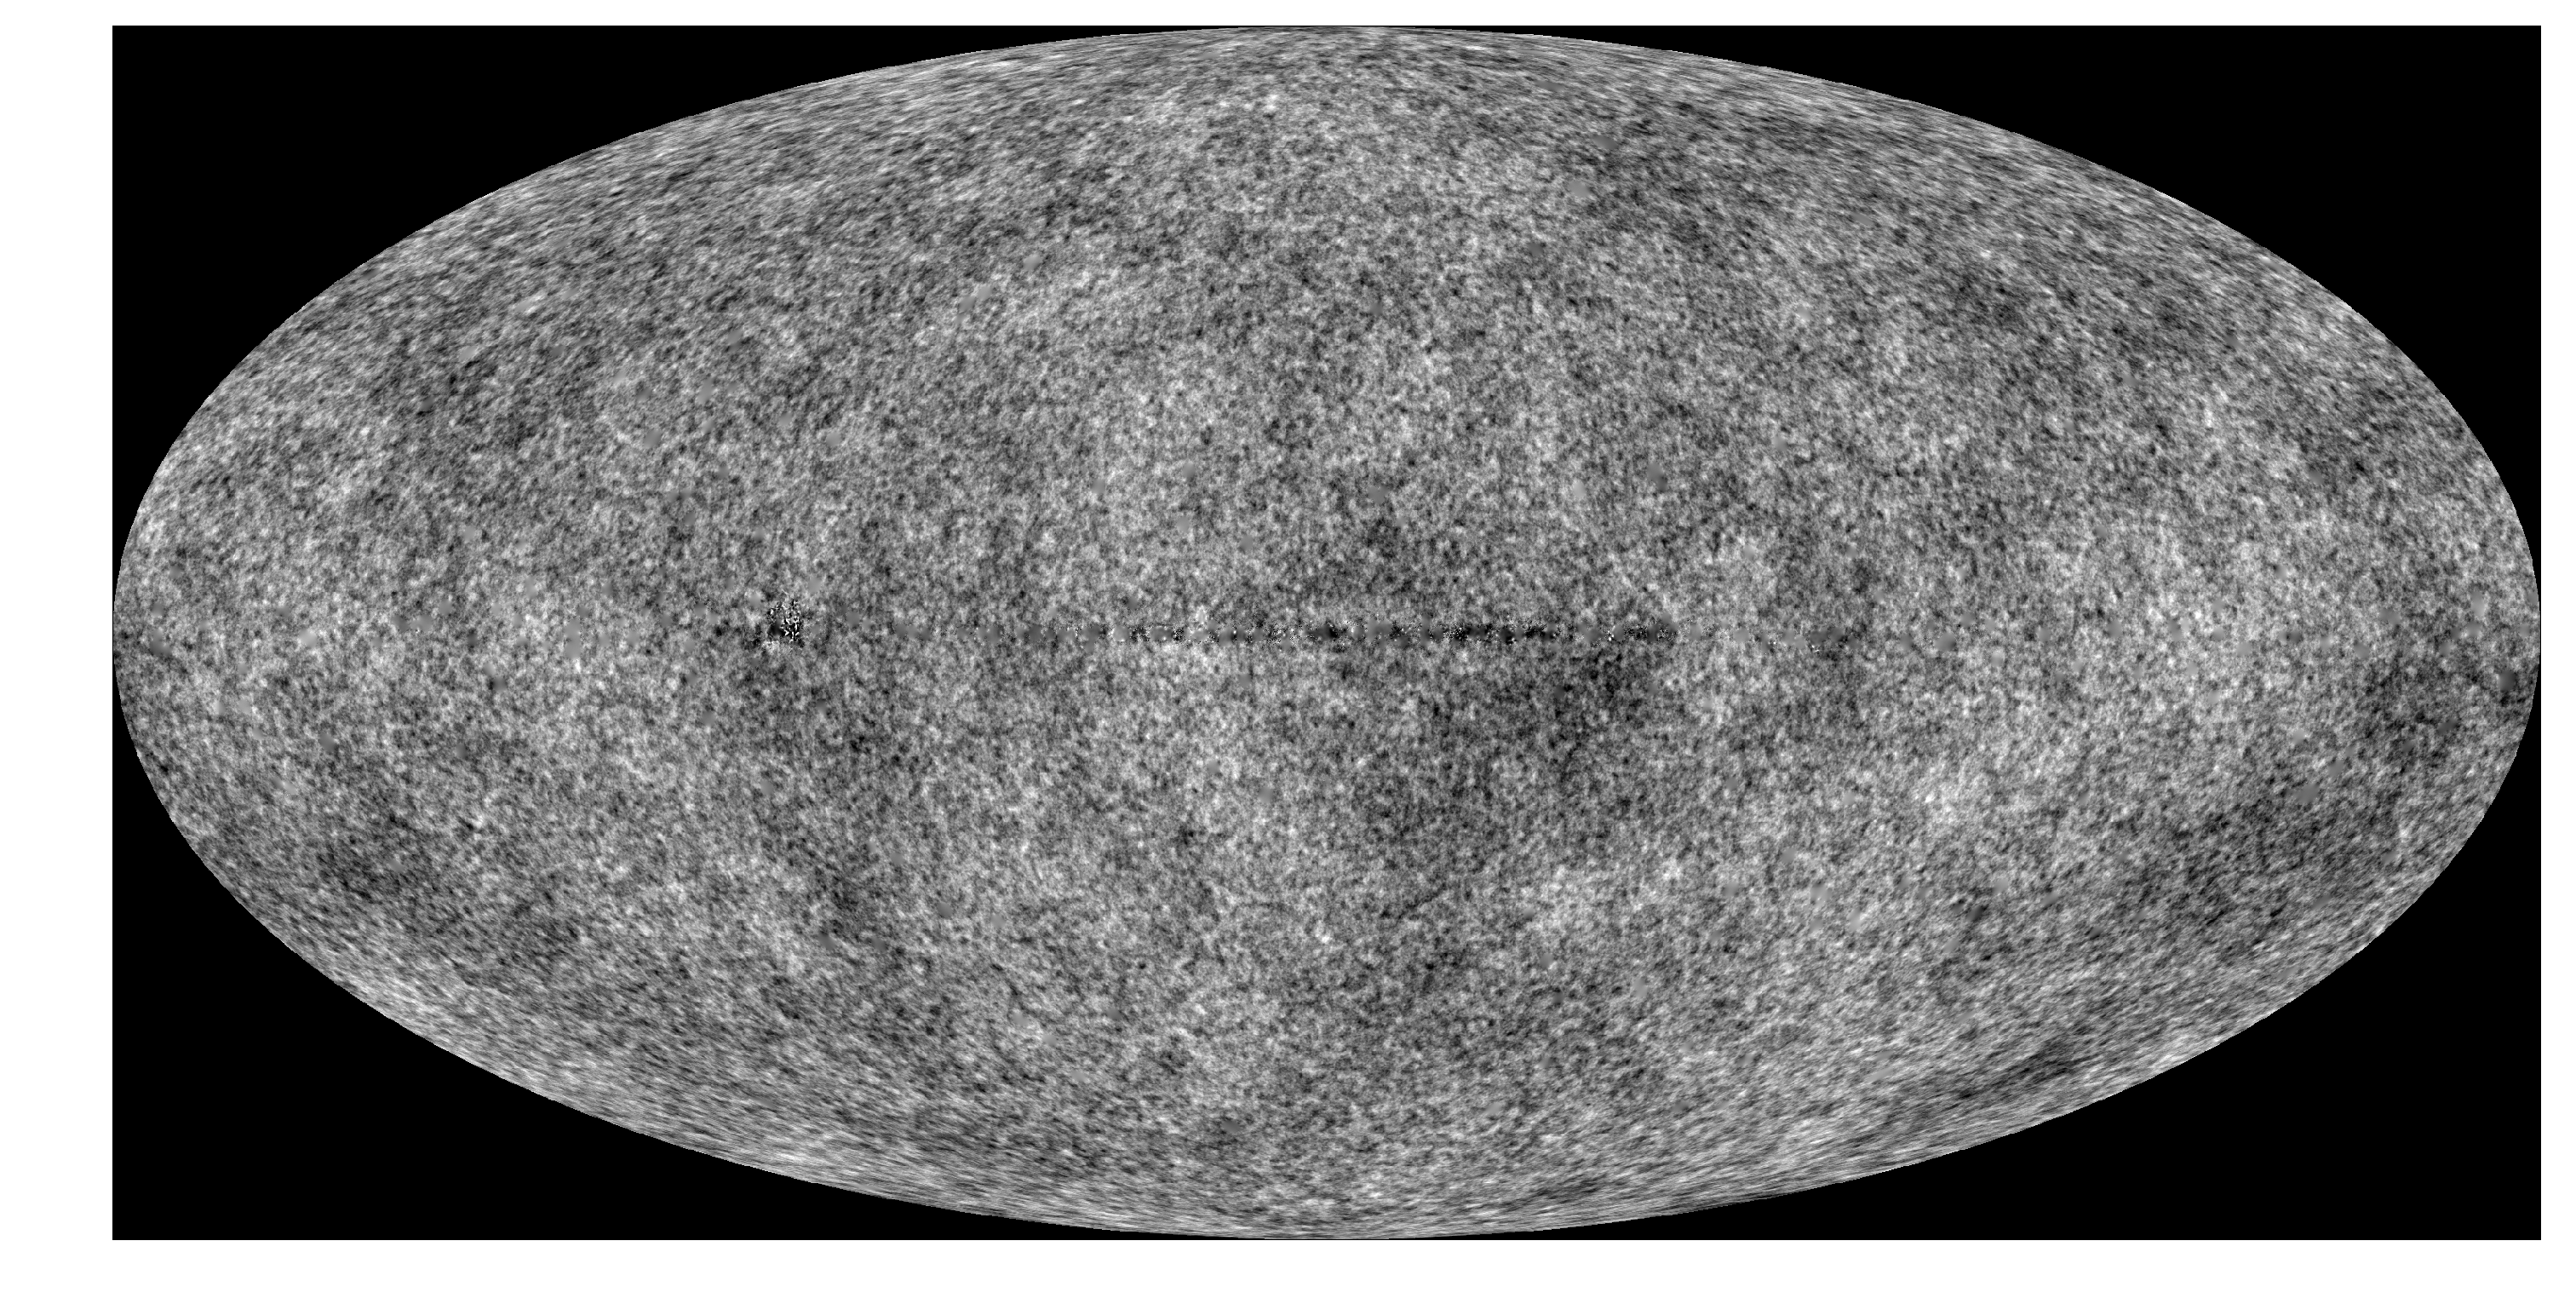
\includegraphics[height=10cm]{figs/planck2015.png}
		\caption[Les fluctuations de température vues par Planck]{La carte des anisotropies de température du fond diffus obtenue par la mission européenne \textit{Planck}. Les zones claires sont plus chaudes que les zones sombres. Le niveau des fluctuations représentées est de l'ordre de 0.001\%.}
	\label{f:planckmap}
\end{figure}

\subsection{Principe de l'analyse des anisotropies du CMB}
Dans cette section, nous allons exposer rapidement les grands principes de l'analyse du signal du fond diffus. Le CMB se manifeste pour l'observateur comme un signal sur tout le ciel, généralement sous la forme d'une carte de température $\delta T(\theta,\phi)$, mesurée dans un repère sphérique. Afin de pouvoir extraire de l'information de ce type de données, l'on raisonne généralement sur la transformée de Fourier\index{transformée de Fourier} de ce signal. Cette opération permet d'une part de séparer les contributions des différentes échelles angulaires\index{echelles@échelles angulaires}. D'autre part, nous verrons que la théorie qui permet de prédire les propriétés de ces fluctuations se fait naturellement dans l'espace de Fourier, où les différentes échelles angulaires évoluent de façon découplée en très bonne approximation.  

Dans un espace sphérique, les opérations de transformées de Fourier s'effectuent via la base des harmoniques sphériques\index{harmoniques sphériques} $Y_{\ell,m}(\theta,\phi)$ et la carte de températures se décompose de la façon suivante:
\begin{equation}
\delta T(\theta,\phi)= \sum_{\ell=0}^{\infty}\sum_{m=-\ell}^{\ell} a_{\ell,m} Y_{\ell,m}(\theta,\phi),
\end{equation}
où les coefficients (complexes) $a_{\ell,m}$ sont obtenus par projection de la carte sur la base vectorielle composée des harmoniques\sidenote[][-2cm]{les harmoniques sphériques apparaissent aussi en mécanique quantique, car elles sont les fonctions propres de la partie angulaire du laplacien, qui encode l'opérateur de moment angulaire}:
\begin{equation}
a_{\ell,m}=\int \int d\theta d\phi\sin \theta Y^*_{\ell,m}(\theta,\phi) \delta T(\theta,\phi).
\end{equation}
Les coefficients $a_{\ell,m}$ constituent ainsi la contribution de chaque harmonique à la carte de température.

\paragraph{Échelles angulaires}
 Les harmoniques sphériques sont les analogues des modes de Fourier sur la sphère, à savoir une base de sinus et cosinus adaptée à une géométrie sphérique:
\begin{equation}
Y_{\ell,m}\sim e^{im\phi} P_{\ell,m}(\cos \theta).
\end{equation} 
 Le coefficient $\ell$ trace l'échelle angulaire\index{echelle@échelle angulaire} de l'harmonique qui possède ainsi une taille angulaire caractéristique $\theta\sim\pi/\ell$: on parle également de fréquence angulaire où les bas $\ell$ désignent les grandes échelles sur le ciel et les grands $\ell$ les petites échelles. Le coefficient $m$ peut varier entre $-\ell$ et $\ell$ et désigne les différentes orientations indépendantes pour chaque taille angulaire caractéristique: celles-ci sont d'autant plus nombreuses que la fréquence angulaire est élevée. L'harmonique $\ell=0$ correspond au monopole, à savoir un signal uniforme sur toute la sphère et dont le coefficient $a_{00}$ renvoie directement à la moyenne sur tout le ciel. Les harmoniques $\ell=1$ sont des dipôles\index{dipôle}, avec un côté «chaud» et un côté «froid» diamétralement opposés. Celles avec $\ell=2$ désignent un quadrupôle, etc.

\paragraph{Spectre de puissance}
\begin{figure}[htbp]
	\centering
		\includegraphics[height=15cm]{figs/cl2015.png}
		\caption[Le spectre de puissance des anisotropies du fond diffus cosmologique obtenu par \textit{Planck}.]{Le spectre de puissance des anisotropies du fond diffus cosmologique obtenu par \textit{Planck}, $D_\ell=\ell(\ell+1)C_\ell$. Les points sont les données et la ligne représente le spectre prévu pour un modèle $\Lambda$CDM. Notez le changement d'échelle horizontale à partir de $\ell=30$.}
	\label{f:cl}
\end{figure}

Armé de la collection des coefficients $a_{\ell,m}$ d'une carte du ciel, on évalue les contributions relatives de chaque échelle par le spectre de puissance angulaire:
\begin{equation}
C_\ell=\langle |a_{\ell,m}|^2\rangle=\frac{1}{2\ell+1}\sum_{m=-\ell}^{\ell} |a_{\ell,m}|^2
\end{equation}
Ce faisant, on rassemble pour chaque échelle angulaire $\ell$ les contributions de toutes les orientations $m$ associées. Si toutes les directions sont à priori équivalentes et aucune n'est privilégiée, alors cette opération ne produit pas de perte d'information. C'est le cas du CMB, celui-ci étant à priori isotrope\index{isotropie!du fond diffus}. D'autre part, une grande classe de modèles d'Inflation prédit que les fluctuations du fond diffus doivent appartenir à la classe des \textit{champs aléatoires gaussiens}\index{champ aléatoire gaussien} qui sont entièrement définis par leur «variance», ce qui est précisément la nature du spectre de puissance angulaire.

\subsection{Avant-plans}

Avant toute chose, il est important de réaliser qu'une carte brute du ciel aux longueurs d'onde sondées par les missions CMB est soumise à une forte contamination par des avant-plans\index{fond diffus!avant-plan} astrophysiques. Parmi ces avant-plans, le plus spectaculaire est sans contexte la Voie Lactée dont par exemple l'émission  par les poussières ou le rayonnement synchrotron empêchent d'accéder aux fluctuations du CMB en arrière plan\sidenote{les régions du ciel couvertes par la Voie Lactée sont par ailleurs fréquemment ignorées lors des études faites sur le fond diffus, à cause des incertitudes générées par sa présence}. Ces avant-plans peuvent être ajustés, modélisés et pris en compte dans des modèles d'inversion, afin d'extraire le signal d'origine cosmologique des portions du ciel affectées. Notons que ces avant-plans sont également source de recherches dédiées, notamment à propos des propriétés des poussières dans la Voie Lactée.

\paragraph{Dipôle} Le premier niveau d'anisotropie est constitué par le dipôle\index{dipole} du CMB. Il possède une amplitude de l'ordre de 3 mK et résulte du mouvement de l'observateur par rapport à la surface de dernière diffusion. Ce mouvement induit un effet Doppler, fonction de la vitesse de déplacement et qui fait apparaître des zones plus chaudes et plus froides que la moyenne, diamétralement opposées et alignées avec la direction de déplacement. Au premier ordre, la variation de température dans la direction du dipôle obéit à la relation:
\begin{equation}
\left(\frac{\Delta T}{T}\right)_\mathrm{dipole}\sim \frac{v}{c}
\end{equation}
et donne une valeur de vitesse de déplacement $v\sim 330$ km/s pour le barycentre du système solaire. Cette vitesse est la somme notamment de la vitesse de déplacement du Soleil dans la Galaxie et de la Galaxie dans le Groupe Local\sidenote{Par Groupe Local, on désigne le groupe de galaxies auquel la Voie Lactée appartient et constitué de la Voie Lactée, de la galaxie d'Andromède et du Triangle ainsi que de tout un ensemble de galaxies moins massives et galaxies satellites}.

\subsection{Anisotropies intrinsèques}
Les fluctuations de température du CMB tracent des fluctuations de densité de matière. Plusieurs modèles de couplage entre matière et rayonnement existent, mais un grand nombre d'évidences observationnelles pointent vers des fluctuations de type \textit{adiabatiques}\index{fluctuations adiabatiques}. Dans ce mode de couplage, le rapport entre la densité de matière et celle de rayonnement reste constant y compris au sein des fluctuations locales : le fluide de matière ne dérive pas par rapport au fluide de photons. Dans ce cas le rapport des densités reste constant:
\begin{equation}
\frac{n}{n_\gamma}=\mathrm{cste}\rightarrow\frac{\delta n}{n}=\frac{\delta n_\gamma}{n_\gamma}
\end{equation}
Pour la matière, densité de matière et d'énergie sont directement reliées $\epsilon=n m c^2$ \sidenote{avec $\rho=n m$} et
\begin{equation}
\frac{\delta n}{n}=\frac{\delta \epsilon}{\epsilon}=\frac{\delta \rho}{\rho}.
\end{equation}
Pour les photons, nous avons déjà vu que $n_\gamma \sim T^3$ :
\begin{equation}
\frac{\delta n_\gamma}{n_\gamma}=3 \frac{\delta T}{T}.
\end{equation}
D'où il apparaît que les fluctuations de températures tracent les fluctuations de densité via:
\begin{equation}
\left(\frac{\delta T}{T}\right)_\mathrm{adiab}=\frac{1}{3}\frac{\delta n}{n}=\frac{1}{3}\frac{\delta \rho}{\rho}.
\end{equation}
Dans un régime de fluctuations adiabatiques, les régions plus chaudes (respectivement plus froides) que la moyenne correspondent aux régions les plus denses (respectivement moins denses) au même moment. 

Toutefois, les fluctuations de densité produisent également des fluctuations de potentiel gravitationnel qui devront être gravies ou dévalées par les photons du fond diffus au moment de leur émission. Les photons en train de sortir d'un puits (correspondant à une surdensité) seront décalés vers le rouge (perte d'énergie) et ceux en train de dévaler un pic de potentiel (correspondant à une sous densité seront décalés vers le bleu (gain d'énergie) \sidenote{cette sensibilité des photons au champ gravitationnel local est un effet standard de la relativité générale}. Cet effet se nomme \textit{effet Sachs-Wolf}\index{effet Sachs-Wolf}
\begin{equation}
\left(\frac{\delta T}{T}\right)_\mathrm{SW}=-\delta\phi
\end{equation}
où $\delta \phi$ est la fluctuation de potentiel. Par ailleurs, on peut montrer que la variation de potentiel est liée à la fluctuation de densité via $\delta \rho/\rho=2\delta \phi$ ce qui implique que la variation de température \textit{totale} est donnée par :
\begin{equation}
\left(\frac{\delta T}{T}\right)_\mathrm{total}=\left(\frac{\delta T}{T}\right)_\mathrm{SW}+\left(\frac{\delta T}{T}\right)_\mathrm{adiab}=-\frac{1}{3}\delta \phi=-\frac{1}{6}\frac{\delta \rho}{\rho}
\end{equation}
Les points chauds du CMB correspondent à des régions sous-denses de l'Univers au moment de l'émission. La carte de température du CMB est donc une carte de la distribution de matière au même instant. Ces fluctuations se situent à des niveaux de 0.001\%, indiquant par la même que l'Univers était extrêmement homogène au moment de la recombinaison.

\paragraph{Grandes échelles} Reste à expliciter l'origine des fluctuations de densité qui conduisent aux fluctuations de températures. L'examen de la figure \ref{f:cl} permet de distinguer 2 régimes. Le premier régime correspond aux grandes échelles $\ell<30$: ces modes sont plus grands que l'Horizon\sidenote{ce terme désigne la plus grande distance sur laquelle un phénomène physique peut se propager : c'est essentiellement le produit de la plus grande vitesse accessible à un processus avec l'âge de l'Univers à l'instant considéré}\index{horizon} au moment de la recombinaison et tracent les fluctuations les plus primordiales, dont on pense qu'elles sont issues d'une période inflationnaire présente aux tout premiers instants après le Big-Bang. L'étude de ces régions du spectre permet notamment de mesurer l'amplitude des fluctuations inflationnaire\index{inflation} ainsi que le spectre de ces fluctuations. En particulier, les théories inflationnaires indiquent que le spectre de puissance tridimensionnel des fluctuations primordiales doit être invariant d'échelle et de la forme:
\begin{equation}
P(k)\sim k^{n_s}
\end{equation}
avec $n_s$ proche mais différent de 1. Les résultats de \textit{Planck 2015} indiquent que $n_s=0.968\pm0.006$ en accord avec ces théories.

\paragraph{Petites échelles} au-delà de $\ell\sim 30$, le spectre présente un ensemble de modes correspondant à des échelles caractéristiques et qui se manifestent sous forme de pics: on en dénombre 3 principaux suivis d'environs 6 pics d'amplitude décroissante. Ces pics indiquent l'existence d'échelles privilégiées dans la carte des fluctuations: ces échelles résultent d'ondes sonores se propageant dans le plasma au moment de la recombinaison. Ces ondes sonores sont appelées \textit{oscillations baryoniques acoustiques}\index{BAO}\index{oscillation baryonique acoustique} \sidenote{BAO en anglais pour \textit{baryonic acoustic oscillations}} : leur production sera décrite en détail dans le chapitre dédié à la croissance des grandes structures. Ces oscillations se mettent en place pour des échelles sub-horizon d'où leur présence seulement aux petites échelles: la position du premier pic permet ainsi de tracer la taille sur le ciel de l'horizon sonore. Connaissant la taille \textit{intrinsèque} de cet horizon, la mesure de sa taille apparente sur le ciel permet de déduire la géométrie du cosmos le long du parcours des photons (et donc $\Omega_m+\Omega_\Lambda$). Connaissant, le rayon de la surface de dernière diffusion $r_{LSS}$ (donnée par le redshift de la recombinaison) et la taille de l'horizon  sonore $L_H$ à cette époque, l'angle qui sous-tend ces fluctuations est simplement donné par:
\begin{equation}
\theta=\frac{L_H}{r_{LSS}}.
\end{equation}
Si $\theta \neq \frac{L_H}{r_{LSS}}$ la trajectoire des photons du fond diffus est incurvée (cf. Fig \ref{f:cmb_geom}), traçant une géométrie courbée de l'Univers dans l'espace circonscrit par la surface de dernière diffusion : au niveau actuel de précision, on ne détecte toutefois aucun départ à la géométrie plane.
\begin{figure}[htbp]
	\centering
		\includegraphics[height=6cm]{figs/cmb_geom.png}
		\caption[CMB et géométrie]{Les fluctuations les plus grandes sont de l'ordre de la taille de l'horizon au moment de la dernière diffusion, représenté sous la forme d'une ellipse claire. L'observateur perçoit ces fluctuations avec une certaine taille angulaire, représentée par l'ouverture des rayons en tirets. Si la trajectoire des rayons lumineux est incurvée à cause de la géométrie globale de l'Univers, cette taille apparente va surestimer (cas du haut, où la géométrie est sphérique) ou sous-estimer (cas du bas, où la géométrie est hyperbolique) la taille angulaire des fluctuations par rapport à celle attendue. Cette comparaison permet d'estimer le départ à la platitude de la géométrie de l'Univers.  }
	\label{f:cmb_geom}
\end{figure}

Les pics suivants tracent la taille des modes ayant effectué un nombre de battements de plus en plus important entre leur production et l'émission du fond diffus. En particulier, leurs amplitudes relatives permettent de contraindre précisément le couplage entre la matière et le rayonnement et la force de rappel qui permet d'entretenir ces battements. Cette force de rappel est induite par la gravité créée par la matière et la mesure de l'entretien de ces battements permet de contraindre la quantité de matière totale ($\Omega_b$ et $\Omega_m$). 


L'une des grandes leçons apprises par l'étude du CMB est la constatation que $\Omega_m>\Omega_b$ : en particulier, la grande amplitude du 3e pic (et des suivants) ne peut s'expliquer par une matière purement baryonique. Elle nécessite une matière non couplée avec le rayonnement, en quantité significative, \textit{la matière noire}. En l'absence de matière noire\index{matière noire}, le couplage entre matière et rayonnement n'est pas suffisamment important pour garantir un entretien maximal des oscillations baryoniques. Ce couplage imparfait conduit à un amortissement de ces dernières au cours des battements successifs : les échelles les plus petites, celles qui oscillent le plus rapidement voient donc leur amplitude décroître. Dans le spectre de puissance angulaire, cela se manifeste par des pics d'amplitudes de plus en plus faibles pour les hautes fréquences angulaires : on parle d'amortissement Silk\index{amortissement Silk}\sidenote{du nom du physicien qui a mis en évidence cet effet}. Or l'amplitude du 3e pic (et des suivants) est supérieure à celle attendue dans le cas d'une matière  purement baryonique, c.-à-d. en présence uniquement de matière capable d'interagir avec le rayonnement (qui fournit le support de pression). Cet excès d'amplitude peut s'expliquer s’ il existe une force de rappel gravitationnelle supplémentaire, créée par de la masse \textit{qui n'est pas sensible à ce couplage rayonnement matière imparfait}. Cette masse qui n'interagit pas avec le rayonnement est la \textit{matière noire}.

Cette matière noire, pèse, entretient les BAOs et n'interagit pas avec le rayonnement : si elle existe, elle nous est actuellement inconnue. On retrouve également trace d'un effet similaire dans la masse des amas de galaxies, dans la dynamique des galaxies et dans les effets de lentille gravitationnelle\index{lentilles gravitationnelles}.

\subsection{Anisotropies secondaires}
En plus des anisotropies imprimées dans le plasma au moment de la Recombinaison, il existe tout un ensemble d'anisotropies créées par différents processus qui affectent les photons du CMB le long de leur parcours entre la surface de dernière diffusion et leur réception. Nous n'en citerons que 3 ici.

\paragraph{La Réionisation} \index{réionisation}
La Réionisation désigne l'époque à laquelle les premières sources de rayonnement ionisant apparaissent dans l'histoire du cosmos entre 400 millions et 1 milliard d'années après le Big-Bang. Ces sources (essentiellement les premières étoiles et quasars\index{quasar}\sidenote{les quasars sont des objets très brillants, visible en particulier à très grande distance. Ils résultent de l'énergie rayonnée par l'accrétion de matière  par les trous noirs supermassifs qu'on trouve au centre de certaines galaxies.}) vont ioniser à nouveau le gaz cosmique, dans un court laps de temps et vont produire une nuée d'électrons libres susceptibles d'interagir avec les photons du CMB par effet Thomson\index{diffusion Thomson}. Cette interaction va influer sur l'amplitude des fluctuations de température et affecter le spectre du CMB en polarisation aux grandes échelles. Cette interaction se mesure via la profondeur optique Thomson $\tau$:
\begin{equation}
\tau=\int_{z_\mathrm{rec}}^{0} c\sigma_t n_e(z)\frac{dt}{dz}dt
\end{equation}
qui est une mesure du nombre d'interactions entre un photon du CMB et les électrons de la Réionisation. Notons que si la Réionisation est précoce, la densité d'électrons $n_e$ est grande et $\tau$ est grand tandis que si elle est tardive, cette densité sera plus faible par simple dilution cosmologique conduisant à une faible valeur de $\tau$. Les mesures du CMB indiquent que la mi-Réionisation a eu lieu pour $z_\mathrm{reion}\sim8$. Pour l'anecdote, les premières estimations de l'effet de la Réionisation sur le fond diffus cosmologique prédisaient des époques de mi-Réionisation bien plus reculées \sidenote{par le satellite américain WMAP par exemple}, vers $z\sim 17$ : depuis, les estimations successives tendent à faire diminuer cette valeur vers celles que nous connaissons actuellement et plus en accord avec les mesures d'opacité du milieu intergalactique qui mettent une fin de Réionisation vers $z\sim 6$. Paradoxalement, ces mesures de plus en plus précises font du CMB une sonde de moins en moins sensible à la Réionisation : une Réionisation tardive implique une densité électronique plus faible et donc une diffusion Thomson secondaire plus faible, réduisant d'autant l'empreinte du processus sur les photons du fond diffus.

\paragraph{L'effet SZ des amas}\index{effet SZ}
Les amas de galaxies sont les plus grandes structures viriélisées de l'Univers actuel. Ils ont été formés récemment, vers $z\sim 1$, et contiennent typiquement plusieurs milliers de galaxies pour des masses totales approchant les $10^{14}-10^{15} M_\odot$. La masse très importante de ces objets fait que le gaz piégé dans leurs puits de potentiel gravitationnel est chauffé à des températures de l'ordre du million de degrés : à ces températures, le gaz devient un fort émetteur X et est l'objet par exemple de processus d'ionisation collisionnelle. De façon analogue à la Réionisation, les amas constituent des ilots denses d'électrons libres avec lesquels les photons du CMB peuvent interagir à des redshifts $z\sim 1$. On parle d'effet Sunyaev-Zeldovich, qui produit de légères distorsions du spectre du CMB, en redistribuant l'énergie des photons vers de plus hautes valeurs. Les amas de galaxies présents sur le ciel produisent ainsi des anisotropies localisées, permettant même leur découverte dans le fond diffus avant confirmation par des observations X par exemple.

Quantitativement, le spectre du fond diffus cosmologique subit une modification en intensité qui suit :
\begin{equation}
\Delta I \sim g(\frac{h\nu}{k_B T_0}) y
\end{equation}
où $g$ est une fonction connue qui donne la dépendance en fréquence de la distorsion spectrale et où $y$ désigne le facteur de «comptonisation» de l'amas de galaxies :
\begin{equation}
y=\int n_e \frac{k_B T_e}{m_e c^2} \sigma_T d\ell.
\end{equation} 
Ce facteur $y$ décrit la physique interne de l'amas, comme sa densité électronique interne $n_e$ ou sa température électronique $T_e$. Pour un amas typique, ce facteur est petit et de l'ordre de 0.0001. La forme fonctionnelle de la dépendance spectrale de l'effet SZ, $g(x)$ \sidenote{on peut montrer que $g(x)=x^4\frac{e^x}{(e^x-1)^2}(\frac{x}{\tanh (x/2)}-4)$.}, présente un pivot pour une fréquence de l'ordre de 200 GHz, quelle que soit le redshift de l'amas : en deçà de cette fréquence, les photons du fond diffus peuvent être redistribués à des énergies supérieures. Une mesure précise des propriétés du CMB doit donc prendre l'effet SZ des amas en compte, tandis qu'à l'inverse cette distorsion spectrale peut être utilisée pour détecter ces amas dans une carte du fond diffus.
\begin{figure}[htbp]
	\centering
		\includegraphics[height=15cm]{figs/SZ.png}
		\caption[L'effet SZ][-1cm]{La présence de gaz chaud et ionisé dans les amas de galaxies à $z\sim 1$ est à l'origine d'une distorsion du spectre du fond diffus, appelé \textit{effet Sunyaev-Zeldovich}. L'interaction entre les électrons énergétiques dans le gaz chaud intra-amas et les photons du fond diffus redistribue l'énergie de ces derniers vers les hautes énergies. La distorsion associée en intensité spécifique est représentée ici pour un amas de galaxies typique avec une température électronique typique de $k_B T_e \sim 10$ keV. On note que l'amplitude de la distorsion est faible, de l'ordre du millième par rapport à l'intensité non modifiée du fond diffus (divisée ici par 1000 pour une meilleure visibilité) }
	\label{f:SZ}
\end{figure}
Pour finir, notons que si l'amas de galaxies est en mouvement, une distorsion supplémentaire due s'ajoute à la précédente à cause de l'effet Doppler qui modifie la perception de la fréquence des photons du CMB. Cet effet est connu sous le nom d'effet SZ \textit{cinétique} tandis que le précédent est connu sous l'effet d'effet SZ \textit{thermique}. L'effet thermique est lié à l'agitation cinétique des électrons libres de l'amas, tandis que l'effet cinétique est lié au mouvement global de ces électrons, piégés dans l'amas en mouvement. Cet effet cinétique est typiquement au moins 10 fois plus faible que le précédent.


\paragraph{Le lentillage gravitationnel cosmique}\index{lentille gravitationnelle}
Les grandes structures croisées par les photons du CMB au cours de leur parcours entre l'émission et leur réception vont modifier subtilement la distribution sur le ciel des anisotropies primaires par effet de lentille gravitationnelle. Une lentille résulte d'une déformation locale de la métrique par une lentille faite de matière (galaxie, amas, filaments, etc..) qui courbe la trajectoire des rayons lumineux et modifie donc l'apparence des sources d'arrière-plan. Dans le cas du CMB, la lentille est constituée de toutes les grandes structures rencontrées au cours de l'histoire de l'Univers tandis que la source d'arrière-plan est la source la plus reculée imaginable. Cet effet de lentille se manifeste essentiellement aux petites échelles et dans le spectre angulaire en polarisation\sidenote{obtenu à partir de l'intensité du rayonnement polarisé du CMB}, il nécessite donc des expériences CMB de grande résolution pour pouvoir être extrait. Il a récemment été mesuré par les expériences sol tel que le \textit{South Pole Telescope} ou dans l'espace par \textit{Planck}. Cette mesure est extrêmement importante, car elle permet de mesurer de façon quasi indépendante les paramètres cosmologiques à partir de la croissance des grandes structures qui opère à des redshifts différents ($z\sim 2$) de ceux concernant la physique du CMB. Elle permet une forte levée de dégénérescence des paramètres mesurés par les fluctuations de température. Pour l'essentiel, les paramètres contraints par le lentillage du CMB confirment les paramètres $\Lambda$CDM obtenus par le fond diffus.
%!TEX root = /Users/domaubert/Documents/Lectures/cosmologie/cosmo_main.tex

\chapter{Formation des grandes structures}
\label{s:struct}
Les grandes structures de l'Univers\index{grandes structures} désignent de façon générique et tout à la fois la matière diffuse, les galaxies et amas de galaxies qui s'organisent sous l'effet de la gravitation. Aujourd'hui ces grandes structures produisent une distribution de matière 'filamentaire' où des surdensités côtoient des vides, reliées entre elles par des ponts de matériau. Elles résultent de l'action du mécanisme d'instabilité gravitationnelle\index{instabilité gravitationnelle} sur les faibles fluctuations de densité présentes dans l'Univers jeune et tracées par exemple par le CMB. Au cours des 13.8 milliards d'années, des surdensité de 0.001\% parviennent ainsi à croître pour atteindre des contrastes de densité mesurés d'au moins plusieurs centaines dans les galaxies aujourd'hui. Si un grande partie des processus à l'œuvre lors de la formation des grandes structures peuvent être saisis par une approche analytique, le problème ne peut être abordé dans toute sa complexité que via l'utilisation de simulations numériques, dites simulation cosmologiques.

\section{Densité et spectre de puissance}
L'un des objectifs de l'étude de la formation des grandes structures est de prédire comme la matière va s'organiser au cours de l'histoire de l'Univers. La quantité généralement suivie est le contraste de densité\index{contraste de densité} :
\begin{equation}
\delta(x,t) =\frac{\rho-\bar\rho}{\bar\rho}.
\end{equation}
En l'absence de création de masse et dans un Univers homogène et isotrope, la densité moyenne $\bar{\rho}$ est une quantité de référence constante dans l'espace et pour laquelle la variation temporelle est seulement due à la dilution cosmologique \sidenote{dont on rappelle qu'elle fait varier la densité en $a^{-3}$.}

Toutefois, le contraste de densité à une position $x$ donnée et à un instant donné $t$ est finalement porteur d'assez peu d'information cosmologique, puisque l'on cherche à obtenir des contraintes qui ont une valeur 'cosmologique', i.e. globales et génériques. La première étape vers un traitement cosmologique consiste à raisonner dans l'espace de Fourier\index{transformée de Fourier} et à considérer les \textit{modes} $\delta_k(t)$ d'une réalisation donnée de $\delta(x,t)$:
\begin{equation}
\delta(x,t)\sim\int_{k=-\infty}^\infty \delta_k(t) e^{ikx} dk
\label{e:fourdelta}
\end{equation}
L'équation \ref{e:fourdelta} représente la décomposition en série de Fourier du contraste de densité : en pratique cela revient à décomposer le champ de densité en une série de modes sinusoïdaux et dont les contributions des différentes fréquences sont données par $\delta_k$. En plus d'un intérêt mathématique, cette décomposition constitue une mise en pratique de 'cosmologisation' de la densité : on se met à suivre des modes sinusoïdaux délocalisés, de taille caractéristique $\lambda=2\pi/k$ et la position $x$ perd de l'importance en tant que telle. L'amplitude d'un mode $k$ est donné tout simplement par $|\delta_k|^2$: l'étude de cette amplitude et son éventuelle évolution temporelle nous renseigne globalement sur l'évolution des structures d'échelle caractéristique $\lambda$ au cours du temps et sur leurs contribution relatives. Cette amplitude est aussi appelée \textit{puissance} et l'ensemble des puissances de tous les modes $k$ est appelé \textit{spectre de puissance}\index{spectre de puissance}.

\paragraph{Champ aléatoire Gaussien} Le champ de matière cosmologique appartient semble-t-il à la classe des champs aléatoires gaussiens\index{champs aléatoire gaussien}. C'est une prédiction des théories inflationnaires et il semble observationnellement que ce soit le cas : in fine cela constitue une base de travail et éventuellement on pourra être amené à mesure des départs à cette gaussianité. Un champ aléatoire gaussien $\delta(\vec x)$ se caractérise par une densité de probabilité de type:
\begin{equation}
p(\delta(\vec x)) \sim \exp( -\delta (\vec x) C^{-1} \delta (\vec x)),
\end{equation}
où $C$ est une matrice de corrélation, généralement non diagonale. Cette matrice encode les corrélations qui peuvent apparaître dans le champ de matière : celui-ci possède généralement des structures possédant une certaine cohérence spatiale et cette dernière se manifeste en couplant le champ $\delta$ entre différentes positions via $C$ \sidenote{par exemple la structuration de la matière dans l'Univers est telle que les régions denses se trouvent plutôt à proximité d'autres régions denses.}. Une propriété intéressante est que la probabilité de la transformée de Fourier de $\delta (\vec x)$ suit le même type PDF:
\begin{equation}
p'(\delta_{\vec k})\sim \exp( -\delta_{\vec k}^* \tilde C^{-1} \delta_{\vec k}).
\end{equation}
Une propriété encore plus intéressante est que $\tilde C$ est diagonale si $\delta(\vec x)$ est un champ aléatoire gaussien: chaque mode de Fourier peut être suivi statistiquement indépendamment des autres. Par simple inspection, il apparaît que les composantes de cette matrice de corrélation sont les variances des modes:
\begin{equation}
\langle \delta_{\vec k}^* \delta_{\vec k'}\rangle = P(k)\delta_D(\vec k -\vec k')=\langle|\delta_{\vec k}|^2\rangle.
\end{equation}
Cette mesure de la variance ne dépend que la norme $k=|\vec k|$ du mode considéré (plusieurs modes partagent donc la même variance) et constitue le spectre de puissance $P(k)$ du champ de matière.

Cette quantité est destinée à être mesurée au cours du temps et nous renseigne sur la croissance des structures. Si certaines échelles bénéficient d'une croissance plus rapide que d'autres, cela se manifestera par une déformation du spectre de puissance aux échelles concernées.  Si le champ est vraiment un champ aléatoire gaussien, la connaissance de $P(k)$ suffit à complètement le définir : si des corrélations anisotropes sont détectées (dans les relevés de galaxies ou dans le CMB), elles confirmeront soit la nature non-gaussienne\index{non-gaussianité} des fluctuations primordiales soit l'existence de processus physiques qui génèrent de la non-gaussianité \sidenote{notons que le spectre de puissance ne permet pas de mesurer la non-gaussianité. Deux champs, l'un gaussien l'autre non, peuvent partager les mêmes variances. Il faut utiliser des statistiques d'ordres supérieurs pour pouvoir faire cette distinction.}.

Une quantité reliée au spectre de puissance est la fonction de corrélation à deux points\index{fonction de corrélation} $\xi (r)$: elle exprime l'excès de probabilité de trouver de la matière en deux points séparés d'une certaine distance $r$ par rapport à une distribution aléatoire. On peut démontrer que la fonction de corrélation à deux points est simplement la représentation du spectre de puissance dans l'espace des positions (donc sa transformée de Fourier):
\begin{equation}
\xi (r)\sim \int d\vec k P(k) e^{i k r}.
\end{equation}
Notons qu'à nouveau cette excès de probabilité de dépend que de la distance $r$ et non pas d'une orientation ou de positions spécifiques des 2 points considérés. Généralement, la fonction de corrélation à 2 points est utilisée si l'on a une description discrète du champ de densité: c'est le cas par exemple lorsque l'on utilise des galaxies comme traceurs de la matière dans les grands relevés. Si l'on travaille avec un champ continu (comme dans des travaux analytiques), on passe directement dans une représentation en mode de Fourier en utilisant le spectre de puissance $P(k)$: ce dernier présente l'avantage d'explicitement séparer les modes de tailles différentes, là où la fonction de corrélation à 2 points "mélange" les modes et peut donc être dominé par une échelle au détriment des autres, qui peuvent pourtant contenir une information pertinente.

\section{Longueur de Jeans}
Une quantité centrale dans l'étude de l'instabilité gravitationnelle est la longueur de Jeans\index{longueur de Jeans}, notée $\lambda_J$. Elle correspond à la longueur minimale  que doit avoir une structure pour s'effondrer sous l'effet de la gravitation. On y associe également une masse (la masse de Jeans\index{masse de Jeans}) $M_J$ donnée simplement par:
\begin{equation}
M_J=\frac{4\pi}{3}\bar\rho\lambda_J^3,
\end{equation}
,où $\bar \rho$ est la densité moyenne du milieu : une structure de masse supérieure à la masse de Jeans va s'effondrer. L'existence du grandeur critique pour que l'effondrement se réalise traduit l'existence d'une compétition entre la gravité et un autre processus que la gravité doit 'vaincre' pour que la structure collapse. En général cet autre processus est l'existence d'un support thermique qui fournit une pression à même de s'opposer à la gravitation. Pour du gaz, il s'agit généralement de la pression interne du gaz, pour des systèmes non-collisionnels (type gaz d'étoiles) c'est la dispersion de vitesse interne qui agit comme une barrière à l'effondrement.

L'expression de la longueur de Jeans peut s'obtenir avec un simple raisonnement: pour qu'une structure s'effondre il faut que l'information gravitationnelle se répartisse plus rapidement au sein d'une structure que l'information de support thermique. Dans un milieu de densité $\rho$ l'information gravitationnelle est transportée en un temps dynamique\index{temps!dynamique}
\begin{equation}
t_G\approx \frac{1}{\sqrt{G\rho}}.
\end{equation}
Pour un gaz la transmission de l'information de support thermique dépend de la vitesse du son\index{vitesse!du son} $c_s$ et de la taille de la structure $\lambda$:
\begin{equation}
t_p\approx\frac{\lambda}{c_s}.
\end{equation}
L'effondrement a lieu si $t_G<t_p$, donc si la taille de la structure considérée obéit à la condition:
\begin{equation}
\lambda >\frac{c_s}{\sqrt{G\rho}}\equiv \lambda_J.
\end{equation}
Faire baisser $\lambda_J$ revient à favoriser l'effondrement gravitationnel, le cas limite étant $\lambda_J \rightarrow 0$ où toute structure s'effondre. Ce régime s'obtient dans un milieu très dense ou bien très froid, i.e. sans support thermique.  A l'inverse, une grande valeur de $\lambda_J$ réduit la possibilité d'effondrement et $\lambda_J\rightarrow\infty$ revient à empêcher toute structure de s'effondrer: cela correspond à un milieu sous-dense, donc très léger, ou bien très chaud avec une grande vitesse du son. Pour un système non-collisionnel, la même expression existe pour la longueur de Jeans en remplaçant la vitesse du son par la dispersion de vitesse du milieu.

\subsection{Traitement perturbatif}
Une dérivation plus rigoureuse peut être obtenue par un traitement perturbatif au premier ordre. On considère un gaz de densité moyenne $\bar \rho$ et d'équation d'état:
\begin{equation}
\frac{dP}{d\rho}=c_s^2.
\end{equation}
Ce gaz obéit aux équation de Poisson\index{equation@équation!de Poisson}, qui est l'équation de champ de la gravité newtonienne:
\begin{equation}
\Delta \phi(x,t) = 4 \pi G \rho
\end{equation}
 et aux équations fluides, conservation de la masse\index{conservation de la masse}
 \begin{equation}
 \frac{\partial \rho}{\partial t} + \vec \nabla \rho \vec u=0,
 \end{equation}
 et conservation de l'impulsion\index{conservation de l'impulsion}
 \begin{equation}
 \frac{\partial \vec v}{\partial t} +\vec u \vec \nabla \vec u = -\frac{\vec \nabla P}{\rho}-\vec \nabla \phi.
 \end{equation}
 On réalise un traitement perturbatif (à 1D par simplicité)\sidenote{notons qu'on considère ici que le milieu n'est pas animé d'une vitesse globale à l'équilibre $v_0=0$ et que le milieu à l'équilibre ne présente pas de variations spatiales de potentiel : ce potentiel $\phi_0$ constant dans l'espace est sans influence dynamique et est donc ignoré}:
 \begin{eqnarray}
 \rho(x,t)&=&\bar \rho(1 +\delta(x,t))\\
 u(x,t)&=&v_1(x,t)\\
 \phi(x,t)&=&\phi_1(x,t)\\
 P&=&P_0+P_1(x,t)
 \end{eqnarray}
 En injectant ces développement, on parvient aisément à écrire:
 \begin{eqnarray}
 \frac{\partial \delta}{\partial t}&=&-\bar \rho \frac{\partial v_1}{\partial x}\\
 \frac{\partial}{\partial t}\frac{\partial v_1}{\partial x}+\frac{c_s^2}{\bar \rho}\frac{\partial^2 \delta}{\partial x^2}+\frac{\partial^2 \phi_1}{\partial x^2}&=&0
 \end{eqnarray}
 d'où l'équation maîtresse de l'instabilité:
 \begin{equation}
 \ddot \delta -c_s ^2\frac{\partial^2 \delta}{\partial x^2}=4\pi G \bar \rho \delta
 \end{equation}
 \subsection{Effondrement et Oscillations}
 Cette équation s'analyse plus facilement en prenant sa transformée de Fourier spatiale:
 \begin{equation}
 \ddot \delta_k +(c_s^2k ^2-4\pi G \bar \rho) \delta_k= 0.
 \end{equation}
 Deux régimes peuvent être facilement distingués:
 \begin{itemize}
 \item si $c_s^2 k^2> 4\pi G \bar \rho$ c'est une équation d'oscillateur harmonique. Le mode correspond à une onde sonore de pulsation $\omega=\sqrt{c_s^2 k^2-4\pi G \bar \rho}$. Cela correspond à des grandes fréquences spatiales, donc des petites structures: notons que leur fréquence temporelle est d'autant plus grande que ces structures sont petites.
 \item si $c_s^2 k^2< 4\pi G \bar \rho$, la solution est hyperbolique avec donc une contribution exponentielle croissante, qui correspond à l'instabilité gravitationnelle. Ce régime correspond aux faibles valeurs de $k$ donc aux grandes échelles. Le temps caractéristique d'instabilité est $\tau = (4\pi G \bar \rho - c_s^2k^2)^{-1/2}$ qui se résume au temps dynamique si k est suffisamment faible donc si le mode étudié est suffisamment grand. 
 \end{itemize}
 
 On remarque que le cas critique $\frac{4\pi^2c_s^2}{\lambda^2}=4\pi G \rho$ nous redonne la longueur de Jeans:
 \begin{equation}
 \lambda_J=c_s\sqrt{\frac{\pi}{G\rho}}
 \end{equation}
 
 \subsection{Cas cosmologique}
\newthought{Le cas cosmologique} se doit de prendre en compte l'expansion de l'Univers. Comme on le verra en fin de démonstration, cela change finalement peu de choses par rapport au cas exposé précédemment. Toutefois cette étude présente un intérêt technique en rapport avec la manipulation de grandeur comobiles dans des équations différentielles couplées. Pour cette raison le calcul sera décrit en détail.

\newthought{Les équations importantes} sont les mêmes que dans le cas d'un Univers statique\sidenote{$\rho$ est la densité de matière, $\vec u$ la vitesse, $\vec  r$ la position physique, $P$ la pression et $\phi$ le potentiel gravitationnel}:
\begin{eqnarray}
\frac{\partial \rho}{\partial t}+\frac{\partial \rho \vec u}{\partial \vec r}&=&0\\
\frac{\partial \vec u}{\partial t}+\vec u \cdot \frac{\partial \vec u}{\partial \vec r}&=&-\frac{1}{\rho}\frac{\partial P}{\partial \vec r}-\frac{\partial \phi}{\partial \vec r}\\
\frac{\partial^2 \phi}{\partial \vec r^2}&=&4\pi G \rho.
\end{eqnarray}
 La principale difficulté découle de la dépendance temporelle de la distance physique\index{distance!physique} $\vec r=a(t) \vec x(t)$ où $\vec x$ désigne la position comobile\index{distance!comobile} : la dérivée par rapport à $\vec r$ doit donc être prise avec précaution. Par commodité on préfère généralement écrire ces équations en fonction de données comobiles pour extraire au moins l'effet de flot cosmologique encodé par le facteur d'expansion $a(t)$.
 
La première étape consiste à transformer les dérivée temporelles prises à $\vec r$ constant en dérivée prises à $\vec x$ constant\sidenote{on rappelle que pour $f(r=a(t)x,t)$ alors $\left(\frac{\partial f}{\partial t}\right)_x=\left(\frac{\partial f}{\partial t}\right)_r+\frac{\partial f}{\partial \vec r}\frac{\partial \vec r}{\partial t}$}:
\begin{equation}
\left(\frac{\partial }{\partial t}\right)_r = \left(\frac{\partial }{\partial t}\right)_x-\frac{\dot a}{a}\vec x \cdot \left(\frac{\partial}{\partial \vec x}\right)_t,
\end{equation}
de même les dérivée spatiales deviennent:
\begin{equation}
\frac{\partial }{\partial \vec r}=\frac{1}{a}\frac{\partial}{\partial \vec x}.
\end{equation}
 Pour finir, il faut établir que la vitesse comporte une partie liée au flot de Hubble\index{Hubble!flot} \sidenote{ le terme $\dot a \vec x$ peut facilement se réecrire sous la forme $H \vec r$, i.e. la loi de Hubble}:
\begin{equation}
\dot {\vec u}=\dot a \vec x + a \dot {\vec x}= \dot a \vec x + \vec v
\end{equation}
 où $\vec v$ désigne une vitesse particulière superposée au flot cosmologique.
 Enfin la densité sera également exprimée en fonction de la densité de fond, $\bar \rho \sim a^{-3}$ qui subit l'expansion cosmologique :
 \begin{equation}
 \rho(\vec x,t) =\bar \rho(t)(1+\delta(\vec x,t)).
 \end{equation}
 
 \newthought{La conservation de la masse} est modifiée comme suit : nous allons prendre les différents termes un par un. La dérivée temporelle de la densité comprend 2 termes, le premier \sidenote{notez la dérivée temporelle de $\bar \rho\sim a^{-3}$ qui intervient ici }:
 \begin{eqnarray}
  \left(\frac{\partial \rho}{\partial t}\right)_x&=& \left(\frac{\partial \rho}{\partial t}\right)_r,\\
  &=&\bar \rho\frac{\partial \delta}{\partial t} -3\frac{\dot a}{a}\bar \rho (1+\delta),
 \end{eqnarray}
et le second:
\begin{eqnarray}
\frac{\dot a}{a}\vec x \cdot \frac{\partial \rho}{\partial \vec x}&=&\frac{\dot a }{a}\bar \rho \frac{\partial\delta}{\partial \vec x}.
\end{eqnarray}
Le terme de flux de cette même équation devient quant à lui:
\begin{eqnarray}
\frac{1}{a}\frac{\partial}{\partial \vec x}(\bar \rho(1+\delta)(\vec v + \dot a \vec x))&&\\
=\frac{\bar \rho}{a} \frac{\partial}{\partial \vec x}(\bar \rho(1+\delta)\vec v) + \frac{\bar \rho \dot a}{a} \frac{\partial}{\partial \vec x}(\bar \rho(1+\delta)\vec x)&&.
\end{eqnarray}
Le dernier terme de cette égalité peut être réecrit sous la forme:
\begin{eqnarray}
\frac{\bar \rho \dot a}{a} \frac{\partial}{\partial \vec x}(\bar \rho(1+\delta)\vec x)&&\\
=\bar \rho \frac{\dot a }{a} 3(1+\delta) +\bar \rho \frac{\dot a }{a} \vec x \cdot \frac{\partial \delta}{\partial \vec x}.
\end{eqnarray}
En rassemblant le tout on obtient l'équation de conservation de la masse dans sa formulation comobile:
\begin{equation}
\frac{\partial \delta}{\partial t}+\frac{1}{a}\frac{\partial}{\partial \vec x}((1+\delta)\vec v)=0
\end{equation}

 \newthought{L'équation d'Euler comobile} \index{equation@équation!d'Euler} se dérive de la même manière. Prenons le premier terme de dérivée temporelle de la vitesse:
 \begin{eqnarray}
 \left(\frac{\partial \vec u}{\partial t}\right)_r&=&\left(\frac{\partial \vec u}{\partial t}\right)_x-\frac{\dot a }{a}\vec x \cdot \frac{\partial \vec u}{\partial \vec x}.
\end{eqnarray}  
La dérivée temporelle à $\vec x$ constant donne:
\begin{eqnarray}
\left(\frac{\partial \vec u}{\partial t}\right)_x&=&\left(\frac{\partial \vec v}{\partial t}\right)_x + \ddot a {\vec x},
\end{eqnarray}
tandis que le terme de Hubble donne \sidenote{on utilise ${\vec e} \cdot \frac{\partial}{\partial \vec x}\vec x= \vec e$}:
\begin{eqnarray}
\frac{\dot a }{a}\vec x \cdot \frac{\partial \vec u}{\partial \vec x}&=&\frac{\dot a }{a}\vec x \cdot \frac{\partial \vec v}{\partial \vec x}+\frac{\dot a^2}{a}\vec x.
\end{eqnarray}
 Le terme d'advection ne présente pas de difficulté particulière \sidenote{on utilise ${\vec e} \cdot \frac{\partial}{\partial \vec x}\vec x= \vec e$} :
 \begin{eqnarray}
 \vec u \cdot \frac{\partial \vec u}{\partial \vec r}&=&\frac{1}{a}\vec v \cdot \frac{\partial \vec v}{\partial \vec x}+\frac{\dot a}{a}\vec x \cdot \frac{\partial \vec v}{\partial \vec x}\\
 &&+ \frac{\dot a^2}{a}\vec x +\frac{\dot a}{a}\vec v.
 \end{eqnarray}
 En rassemblant tous ces premiers termes on obtient une expression comobile pour le membre de gauche de l'équation d'Euler:
 \begin{equation}
 \left(\frac{\partial \vec v}{\partial t}\right)_x +\frac{\dot a}{a}\vec v+\frac{1}{a}\vec v \cdot \frac{\partial \vec v}{\partial \vec x} + \ddot a {\vec x}. 
 \label{e:geuler}
 \end{equation}
 Le terme correspondant aux forces de pressions\index{pression} de pose pas de difficulté tandis que le terme correspondant aux forces de gravitation peut être modifié en lui incluant le terme en $\ddot a {\vec x}$ de l'équation \ref{e:geuler}:
 \begin{eqnarray}
  \frac{\partial \phi}{\partial \vec r}&=&\frac{1}{a}(\frac{\partial \phi}{\partial \vec x}+a\ddot a \vec x)\\
  &=&\frac{1}{a}\frac{\partial \Phi}{\partial \vec x},
 \end{eqnarray}
 où $\Phi(\vec x,t)$ est un potentiel gravitationnel effectif, prenant en compte les effets de fonds changeant:
 \begin{equation}
 \Phi= \phi+\frac{a\ddot a {\vec x}^2}{2}.
 \end{equation}
En rassemblant partie différentielle et termes sources, on obtient une équation d'Euler comobile qui ressemble beaucoup à sa contrepartie physique avec l'inclusion d'un terme de friction de Hubble :
\begin{equation}
\left(\frac{\partial \vec v}{\partial t}\right)_x +\frac{\dot a}{a}\vec v+\frac{1}{a}\vec v \cdot \frac{\partial \vec v}{\partial \vec x}=-\frac{1}{a\bar \rho (1+\delta)}\frac{\partial P}{\partial \vec x}-\frac{1}{a}\frac{\partial \Phi}{\partial \vec x}.
\end{equation}

\newthought{L'équation de Poisson}\index{equation@équation!Poisson} doit également être reformulée en faisant notamment intervenir le potentiel effectif $\Phi$\sidenote{en utilisant $\frac{\partial^2}{\partial \vec x^2} {\vec x}^2=6$}:
\begin{eqnarray}
\Delta \phi &=&\frac{1}{a}\frac{\partial^2 \phi}{\partial \vec x^2}\\
&=&\frac{1}{a^2}\frac{\partial \Phi}{\partial \vec x^2}-3\frac{\ddot a}{a}\\
&=&4\pi G \bar \rho(1+\delta).
\end{eqnarray}
Or l'équation de Friedmann\index{equation@équation!Friedmann}\sidenote{$\frac{\ddot a}{a}=-\frac{4}{3}\pi G \bar \rho$} permet de relier l'évolution du facteur d'expansion avec la densité du fond et permet notamment d'établir que:
\begin{equation}
4\pi G \bar \rho a^2+3 a \ddot a=0,
\end{equation}
 d'où l'équation de Poisson comobile:
 \begin{equation}
 \frac{\partial^2 \Phi}{\partial \vec x^2}=4\pi G \bar \rho a^2 \delta
 \end{equation}
 
 \newthought{En présence d'expansion}, l'équation maîtresse devient (pour chaque mode de Fourier):
 \begin{equation}
  \ddot \delta_k +2H\dot \delta_k+ (\frac{c_s^2k ^2}{a^2}-4\pi G \bar \rho) \delta_k= 0.
  \label{e:epert}
 \end{equation}
 où toutes les quantités sont des quantités comobiles. On retrouve essentiellement la même équation et les mêmes conclusions s'imposent, à savoir instabilité si $\lambda >\lambda_J$ et oscillations sonores dans le cas inverse. On note toutefois la présence du terme $2H\dot \delta_k$ qui s'apparente à un terme d'amortissement dû à l'expansion. On montrera qu'à cause de ce terme qui tempère les solutions, les modes instables\index{modes instables} ne seront plus exponentiels mais en loi de puissance et les modes stables oscillants seront amortis sur des temps caractéristiques de l'ordre du temps de Hubble.
 
 A ce stade il faut rappeler, que le traitement décrit juste ici est approché. Par exemple la matière noire \sidenote{qui compose $80\%$ du bilan énergétique de la matière} ne peut pas, à priori, être correctement décrite par les équations 'fluides' utilisées ici. Comme ses particules sont non collisionelles, on ne peut réduire la pression\sidenote{qui est une mesure des propriétés du tenseur des dispersions de vitesses} à un scalaire et elle peut être anisotrope. La question se pose dans les même termes pour le rayonnement. Un traitement rigoureux doit passer par l'utilisation de l'équation de Boltzmann qui encode directement l'évolution de la fonction de distribution des ces fluides dans l'espace des phases et non celle des ses moments (densité, impulsion, etc...).  Heureusement le résultat obtenu reste très similaire à celui présenté dans l'équation \ref{e:epert} et elle fera donc l'affaire pour les raisonnements à suivre.
 
 L'autre difficulté est lié à la nature multi-fluide des perturbations. Nous avons:
 \begin{itemize}
 \item les photons: relativistes, avec une pression de rayonnement associée,
 \item les baryons: non-relativistes mais couplés avec le rayonnement avant la recombinaison. Les photons vont donc leur fournir une source de support dynamique bien plus importante que la simple pression thermique,
 \item la matière noire : non-relativiste et sans pression.
 \end{itemize}
 Ces 3 fluides vont évoluer selon des termes donnés par l'éq. \ref{e:epert}. Par ailleurs ces fluides sont couplés et s'influencent l'un l'autre : c'est vrai via la pression de rayonnement pour les baryons et les photons mais également via le terme $4\pi G \bar \rho \delta_k$. Ce terme trace une source gravitationnelle de perturbation et doit donc inclure toutes les contributions au bilan énergétique de l'Univers, photons compris. C'est notamment vrai durant les époques avant l'équivalence \sidenote{correspondant à $z>3000$ ou $t<80 000$ ans où matière et rayonnement contribuent de manière égale au bilan énergétique du cosmos} durant lesquelles la source principale de potentiel est la contribution des photons. En pratique, nous avons donc un jeu d'équations multiples couplées qu'on ne peut résoudre de façon analytique : les grands principes peuvent toutefois être explorés en appliquant des hypothèses raisonnables comme décrit dans les parties suivantes.
 
 \section{Croissance des perturbations : cas sub-horizon}
 \newthought{Les échelles explorées} dans cette partie sont suffisamment compactes pour être plus petites que l'horizon a un instant donné. Cela permet en particulier le transport d'une information dynamique au sein des structures en jeu, autorisant effondrement ou ondes de pression par exemple. L'équation à interpréter est celle donnée par l'eq. \ref{e:epert} et nous allons être amenés à distinguer 2 époques, avant l'équivalence (dominée par le rayonnement RD) et après l'équivalence (dominée par la matière MD). Les facteurs d'expansion et le paramètre de Hubble \sidenote{avec $H=\dot a/a$} durant RD sont donnés par :
 \begin{eqnarray}
 a&\sim& \sqrt{t},\\
 H&=&\frac{1}{2t},
 \end{eqnarray}
 tandis que les relations équivalentes durant MD sont données par:
 \begin{eqnarray}
 a&\sim&t^{2/3},\\
 H&=&\frac{2}{3t}.
 \end{eqnarray}
 
  \subsection{Matière sans pression}
Prenons d'abord le cas d'une matière sans pression, correspondant à celui de la matière noire : la vitesse du son est négligeable et pourra donc être annulée dans Eq. \ref{e:epert}.

\newthought{Durant l'époque dominée par le rayonnement}, le terme source de gravitation est dominé par la contribution des photons. Toutefois, on considèrera ce terme comme négligeable : les photons possèdent une pression intrinsèque élevée et une grande longueur de jeans. Ils ne peuvent se structurer et leur densité ne peut croître de façon substantielle \sidenote{de fait elle aura un comportement oscillant, voir section suivante}:
\begin{equation}
\bar \rho \delta_k \sim(\bar \rho \delta_k)_\gamma \sim 0.
\end{equation}
L'équation résultante pour la matière sans pression est donc: 
\begin{equation}
\ddot \delta_k+\frac{1}{t}\dot \delta \sim 0
\end{equation}
dont la solution est de type logarithmique:
\begin{equation}
\delta_{k,RD}\sim \log(t).
\end{equation}
Dans le cadre qui est le nôtre, une croissance logarithmique peut être assimiliée à une absence de croissance, au mieux à une croissance très lente.

\newthought{Durant l'époque dominée par la matière}, le terme source est dominé par la matière elle-même: toute croissance sera donc entretenue par une croissance du potentiel, conduisant naturellement à une augmentation de la perturbation. L'équation à traitée est donnée par:
\begin{equation}
\ddot \delta_k +2 H \dot \delta_k =4\pi G \bar\rho \delta_k.
\end{equation}
En introduisant explicitement les dépendances temporelles on obtient\sidenote{en utilisant $\bar \rho\sim\rho_c=\frac{3H^2}{8\pi G}$}:
\begin{equation}
\ddot \delta_k +\frac{4}{3t}\dot \delta_k - \frac{2}{3t^2}\delta_k=0.
\end{equation}
Cette équation possède une solution croissante donnée par \sidenote{il existe aussi une solution décroissante en $\delta=1/t$, qui est de peu d'intérêt car dominée par la solution croissante} :
\begin{equation}
\delta_{k,MD}\sim t^{2/3}\sim a(t).
\end{equation}
Le contraste avec la solution précédente est frappant: la présence d'un terme source de gravitation permet à la fluctuation de prospérer tandis que que son absence conduit à une non-augmentation de la perturbation.

\subsection{Matière avec pression}
Ce cas correspond à celui des baryons : durant ces époques pré-recombinaison, le couplage important entre les photons et les baryons confère à ces dernier une pression importante et une vitesse du son proche de la vitesse de la lumière $c_s\sim c$.

\newthought{Durant l'époque dominée par le rayonnement}, on continuera à négliger le terme source induit par les photons par contre le terme de pression ne peut plus être omis et l'équation des perturbations devient:
\begin{equation}
\ddot \delta_k+2H\dot \delta +c_s^2k^2 \delta \sim 0.
\end{equation}
La solution est oscillante avec un amortissement induit par l'expansion\sidenote{avec un temps caractéristique $\tau \sim{1/2H}$.}. De notre point de vue, c'est également une solution 'sous contrôle', non-croissante. En l'absence de gravitation, les fluctuations baryoniques s'organisent en ondes de pression.

\newthought{Durant l'époque dominée par la matière}, le terme source de gravitation devient non négligeable mais n'est pas dominé par les baryons\sidenote{qui ne représente que $20\%$ de la matière totale}. L'équation à résoudre devient alors \sidenote{ici $DM$ dénote la matière noire pour \textit{dark matter}.}:
\begin{equation}
\ddot \delta_k+2H\dot \delta +c_s^2k^2 \delta 4\pi G \bar\rho_{DM} \delta_{k,DM}
\end{equation}
On a donc un terme source de fond, mais ce terme n'est pas en mesure de produire une augmentation de l'amplitude des oscillations: ce terme évolue lentement par rapport aux temps caractéristiques d'oscillations et ne peut donc produire de résonances par exemple. Ce terme de forçage n'implique pas de croissance incontrôlée de l'amplitude des fluctuations baryoniques qui sont toujours dans un régime oscillant comme précédemment.

\newthought{Ces oscillations} constituent de notre point de vue une 'absence de croissance': les ondes de pressions passent mais ne 'grossissent pas'. En pratique c'est même l'opposé qui va se produire : à cause du couplage imparfait entre photons et rayonnement, la pression apportée par les photons ne garantit pas un entretien perpétuel des oscillations et elles vont s'amortir \sidenote{on parle aussi d'amortissement Silk\index{amortissement Silk}, du nom du physicien anglais à l'origine de la découverte de cet effet}. L'effet d'amortissement est même catastrophique au sens où toute structure baryonique contenant une masse inférieure à $10^{13} M_\odot$ \sidenote{et donc de taille inférieure à une certaine taille critique} doit être 'effacée' du spectre des fluctuations. Cette masse est supérieure à celle de la Voie Lactée actuellement : il faut donc trouver un mécanisme pour entretenir les fluctuations de masse inférieure à cette limite pour pouvoir expliquer les structures observées aujourd'hui.

\newthought{La matière noire}\index{matière noire} va fournir ce mécanisme: comme vu précédemment, la matière sans pression va voir ses fluctuations croître de façon permanente durant l'époque dominée par la matière. Au moment de la recombinaison, les baryons auront vu une grande partie de leurs fluctuations être amorties par l'amortissement que nous venons juste de mentionner. Toutefois la recombinaison s'accompagne de la perte de support de pression offert par le rayonnement \sidenote{permettant aux photons de s'échapper sous forme du rayonnement de fond diffus}: les baryons sont alors libres de s'effondrer dans les puits de potentiels crées par la matière noire. Vers un redshift $z\sim 100$ les fluctuations baryoniques ont convergé vers les fluctuations de la matière noire, autorisant la formation de structures de masses plus légères que la masse limite mentionnée précédemment.

\begin{figure}[htbp]
	\centering
		\includegraphics[height=12cm]{figs/bao1.png}
	\caption[Les oscillations baryoniques évoluent sur des fréquences différentes, dépendant de leur taille.]{Les oscillations baryoniques évoluent sur des fréquences différentes, dépendant de leur taille. Les grandes structures oscillent lentement, les petites rapidement. Certains modes vont être en extremum d'amplitude au moment de la recombinaison et donc au moment de la dernière diffusion du fond diffus cosmologique. Ces modes vont donc être privilégiés dans la carte du CMB.}
	\label{f:bao1}
\end{figure}


\newthought{Ces oscillations baryoniques}  sont des ondes accoustiques (BAOs, de l'anglais \textit{baryonic accoustic oscillations})\index{BAO} car elles sont entretenues par l'entrejeu entre gravité et pression (de rayonnement dans le cas présent). Par simple inspection de l'équation différentielle maîtresse, on peut constater que la fréquence d'oscillation dépend de la taille du mode étudié : un mode à grande fréquence spatiale implique une grande fréquence temporelle et vice-versa. Par conséquent, l'amplitude du mode au moment de la recombinaison va dépendre du mode en question : au moment de l'émission du fond diffus, certains modes seront en amplitude maximale, d'autres en amplitude plus modérée. En simplifiant (voir Fig. \ref{f:bao1}), on peut imaginer que certains modes vont osciller un nombre de fois exactement entier entre leur déclenchement et la recombinaison, parvenant ainsi à un extremum d'amplitude tandis que d'autres seront dans une phase quelconque avec des amplitudes moins remarquables. Les échelles qui se détachent sous la forme de 'pics' dans le spectre de puissance du fond diffus cosmologique (voir Fig. \ref{f:bao2}) sont la manifestation de ces modes qui parviennent en extremum d'amplitude au moment où le rayonnement fossile est produit.



\begin{figure}[htbp]
	\centering
		\includegraphics[height=12cm]{figs/bao2.png}
	\caption[Les pics accoustiques sont des extrema]{Les pics accoustiques du spectre de puissance du fond diffus cosmologique correspondent aux modes qui sont en extremum d'amplitude au moment de la recombinaison. Le premier pic correspond à une compression, le second une compression + une détente, le troisième une compression + une détente + une compression, etc.... Au premier ordre, nous voyons des harmoniques d'un même mode fondamental. }
	\label{f:bao2}
\end{figure}

\section{Croissance des perturbations : cas super-horizon}

Jusqu'à présent, nous nous sommes concentrés sur les petites échelles. Regardons à présente le comportement d'un mode de très grande taille, dont la longueur caractéristique est plus grande que \textit{l'horizon cosmologique} à l'instant considéré. Ces modes sont appelés super-horizon, tandis que les modes de petite taille précédemment étudié sont par analogie désignés comme étant sub-horizon.

\newthought{L'horizon}\index{horizon} désigne la plus grande échelle sur laquelle un phénomène de propagation peut opérer. Sa valeur est simplement donnée par :
\begin{equation}
L_H=\frac{c}{H}
\end{equation}
où $H^{-1}$ apparaît comme une mesure de l'âge de l'Univers à un instant donné. L'horizon est donc le produit de la plus grande vitesse par la plus grande durée. Son expression comobile présente une évolution temporelle qui dépend de la période de domination. Durant la période dominée par le rayonnement on a comme horizon comobile:
\begin{equation}
\ell_{H,RD}=\frac{c}{aH}\sim a
\end{equation} 
et durant la période dominée par la matière:
\begin{equation}
\ell_{H,MD}\sim\sqrt{a}.
\end{equation}
Dans les 2 cas, l'horizon grandit avec le temps et un mode de taille comobile donnée va donc successivement être plus grand que l'horizon (super-horizon) puis plus petit (sub-horizon) : usuellement, on désigne cette transition par l'expression \textit{passer sous l'horizon}. Le cas super-horizon demande un traitement en relativité générale complet donnant l'équation de croissance des structures suivantes:
\begin{equation}
\ddot \delta_k + 2H \dot \delta_k = \frac{3}{2}H^2(1+w)(1+3w)\delta_k
\end{equation}
où $w=0$ durant l'époque MD et $w=1/3$ durant l'époque RD \sidenote{pour ces échelles plus grandes que l'horizon, la pression ne peut jouer un role significatif: baryons et matière noire ont le même comportement}. 

Cette équation est similaire à celle obtenue dans le cas sub-horizon. Pour l'époque de domination de la matière on retrouve le même taux de croissance que celui obtenu pour la matière noire :
\begin{equation}
\delta_{k,MD}\sim t^{2/3}\sim a(t),
\end{equation}
tandis que durant l'époque de domination du rayonnement on obtient:
\begin{equation}
\delta_{k,RD}\sim t \sim a(t)^2.
\end{equation}


\section{Croissance des perturbations : synthèse et spectre de puissance}

La synthèse des résultats précédents pour le cas de la matière noire est présenté dans la figure \ref{f:perturb}. On constate qu'une petite perturbation peut voir son histoire de croissance gelée si elle passe sous l'horizon durant l'époque dominée par le rayonnement. A l'inverse un mode de grande longueur d'onde devra attendre la période dominée par la matière pour changer de régime et ne connaîtra pas la phase de non-croissance qu'auront connu les plus petites structures.

\begin{figure}[htbp]
	\centering
		\includegraphics[height=8cm]{figs/perturb.png}
		\caption[Synthèse de la croissance des perturbations]{Synthèse de la croissance des perturbations. Un petit mode possède une taille caractéristique suffisemment petite pour passer sous l'horizon durant l'époque dominée par le rayonnement.}
	\label{f:perturb}
\end{figure}

Grâce à cette synthèse on peut prédire l'amplitude d'un mode au moment de la recombinaison $\delta_f$ en fonction de son amplitude $\delta_i$ bien avant l'équivalence matière-rayonnement. Considérons d'abord le cas d'un grand mode, sans période de gel de croissance, son amplitude au moment de l'équivalence est donné par:
\begin{equation}
\delta_e=\frac{a_e^2}{a_i^2}\delta_i.
\end{equation}
Son amplitude finale est alors donnée par :
\begin{equation}
\delta_f=\frac{a_f}{a_e}\delta_e=\frac{a_f a_e}{a_i^2}\delta_i.
\end{equation}
La chose importante est l'indépendance du facteur reliant l'amplitude initiale et finale vis à vis de la taille du mode : tous les modes vont croître dans les même proportions entre les instants $i$ et $f$. 

Pour les petits modes la situation est différente. L'amplitude au passage sous l'horizon est donnée par
\begin{equation}
\delta_L=\frac{a_L^2}{a_i^2}\delta_i.
\end{equation}
où $a_L$ est l'instant de passage sous l'horizon. L'amplitude au moment de l'équivalence est identique car la croissance est gelée et l'amplitude finale est alors donnée par:
\begin{equation}
\delta_f=\frac{a_f}{a_e}\delta_e=\frac{a_f}{a_e}\delta_L=\frac{a_L^2 a_f}{a_i^2 a_e}\delta_i.
\end{equation}
Ici le facteur de lien dépend de $a_L$ et donc de la taille du mode considéré. En effet cet instant est déterminé par $\lambda = \ell_{H,RD} \sim a_L$ donc 
\begin{equation}
\delta_f \sim \frac{1}{k^2} \delta_i.
\end{equation}
On a une coupure d'autant plus forte que la fréquence du mode est élevée, d'autant plus forte que la taille du mode considéré est petite.

\newthought{Pour le spectre de puissance}\index{spectre de Puissance}, les conséquences sont simples. Pour les $k$ suffisamment faibles on a 
\begin{equation}
P_f(k)\sim\delta_k^2 \sim P_i(k),
\end{equation}
par contre pour les hautes fréquences le spectre de puissance est filtré suivant la relation:
\begin{equation}
P_f(k)\sim \frac{1}{k^4} P_i(k)
\end{equation}
Comme le spectre de puissance primordial est en loi de puissance tel que \sidenote{on parle de spectre invariant d'échelle, comme prédit par exemple par l'inflation}:
\begin{equation}
P_i(k)\sim k
\end{equation}
on obtient un spectre caractéristique aux hautes fréquences en 
\begin{equation}
P_f(k)\sim\frac{1}{k^3}.
\end{equation}
Le spectre de puissance résultant possède donc 2 régimes caractéristiques, l'un aux grandes échelles en $P(k)\sim k$ et l'autre aux petites échelles en $P(k)\sim k^{-3}$. La transition entre les deux correspond à l'échelle qui passe sous l'horizon exactement au moment de l'équivalence (cf. Fig \ref{f:pk}).

\begin{figure}[htbp]
	\centering
		\includegraphics[height=8cm]{figs/pk.png}
		\caption[Schématique du filtrage du spectre de puissance des fluctuations initiales.]{Schématique du filtrage du spectre de puissance des fluctuations initiales. Le spectre primordial est invariant d'échelle en $P(k)\sim k$ et le gel de la croissance des fluctuations sous l'horizon durant l'époque de domination du rayonnement produit un filtrage au hautes fréquences qui produit une pente caractéristique en $P(k)\sim k^{-3}$.}
	\label{f:pk}
\end{figure}

\newthought{Pour résumer}, le spectre de puissance de la matière est une version filtrée du spectre de puissance primordial. Ce filtre opère sur les échelles suffisamment petites pour passer dans l'Horizon cosmologique tôt dans l'histoire de l'Univers, durant l'époque dominée par le rayonnement. Les échelles plus grandes ne permettant pas ce passage fréquence ont crû de façon indifférenciée et ont donc conservé les caractéristiques du spectre primordial. L'ensemble des prédictions développées dans ce chapitre, et notamment la mise en place du spectre de puissance $P(k)$ est fermement confirmée par de multiples observations (voir Fig. \ref{f:pktegmark})~: c'est un des grands succès du modèle $\Lambda$CDM aux grandes échelles.

\begin{figure}[htbp]
	\centering
		\includegraphics[height=12cm]{figs/pstegmark.png}
		\caption[Le spectre de puissance observé]{Le spectre de puissance $P(k)$ $\Lambda CDM$ théorique est représenté ici avec une compilation des estimations observationnelles issues de différentes sondes~: lensing, relevés de galaxies, CMB, comptage d'amas, Forêt Lyman-$\alpha$. On note l'excellent accord en théorie et prédiction.  Figure extraite de Tegmark et al. 2003. }
	\label{f:pktegmark}
\end{figure}


\newthought{Les oscillations baryoniques}\index{BAO}, mentionnées dans le cas de la matière avec pression et vues dans le CMB, se manifestent également dans le spectre de puissance de la matière totale. Ces ondes sonores se propageant dans le gaz vont légèrement modifier la structure globale de la matière : même si les baryons ne représentent qu'une faible fraction\sidenote{$\frac{\Omega_b}{\Omega_m}\sim0.15$} de la masse totale, cette fraction est non nulle et joue sur la dynamique globale à l'oeuvre. Ces oscillations se manifestent à nouveau comme des modes légèrement privilégiés dans le spectre de puissance $P(k)$. Par ailleurs, ces modes privilégiés vont persister dans la distribution de matière bien au delà de la recombinaison, jusqu'à nos jours. Par exemple, le spectre de puissance de la distribution actuelle des galaxies\sidenote{mesurée à z=0 dans des grands relevés de millions de galaxies comme le Sloane Digital Sky Survey (SDSS)}  présente des modes privilégiés aux fréquences attendues (voir Fig. \ref{f:percival}). De même, la distribution du gaz diffus intergalactique\index{IGM} à z=2\sidenote{sondée dans les spectres de Quasars distant} manifeste ces mêmes modes privilégiés. Ces ondes de pression primordiales, ont laissé leur empreinte dans toutes les structures qui ont émergé tout au long de l'histoire de l'Univers.

\begin{figure}[htbp]
	\centering
		\includegraphics[height=12cm]{figs/percival.png}
		\caption[Les BAOs dans les relevés de galaxies]{Détection des BAOs dans le spectre de puissance du grand relevé de galaxies SDSS. Les courbes représentées sont le rapport du spectre mesuré dans les données sur le spectre lissé, sans BAO, pour 3 échantillons de galaxies différents. Les BAOs sont très clairement apparent (points) aux positions prédites par la théorie (lignes). Figure extraite de Percival et al. 2007.}
	\label{f:percival}
\end{figure}

\section{Et après ?}

Une fois le mécanisme d'instabilité déclenché, tous les modes vont parvenir à des régimes de surdensité qui vont au delà du régime linéaire et qui sortent du cadre dans lequel nous nous sommes placés. Dans certains cas académiques, le régime non linéaire peut-être abordé analytiquement mais en toute généralité il requiert l'utilisation de simulations numériques. La culmination de ce régime non linéaire est la création de structure denses, dominées par les baryons et au sein duquel se forment les sources de rayonnement : ce sont les galaxies qui nous entourent. L'apparition de ces objets est donc conditionnée par un contexte cosmologique et par extension il n'est pas illogique d'affirmer que l'étude de la formation des galaxies est une extension naturelle de la cosmologie. Toutefois, des phénomènes astrophysiques commencent à rentrer en jeu aux échelles considérées : thermodynamique du gaz, processus physico-chimique de refroidissement, champ magnétique, formation et rétroaction stellaire, production et impact des éléments plus lourds que l'hélium, etc.... Chacun de ces phénomènes est un objet d'étude à part entière et chacun de ces phénomènes est compris de façon toute relative. On en décrira quelques-uns ci-dessous, mais de façon générale on peut aisément avancer qu'aujourd'hui l'extension de la théorie cosmologique à celle de la formation des galaxies présente des défis majeurs. Ces défis, à l'heure où ces lignes sont écrites ne sont pas résolus.

\chapter{Formation des 'petites' structures}

\section{Au-delà du régime linéaire : le modèle d'effondrement sphérique}

\newthought{Une surdensité de matière} va nécessairement sortir du régime des faibles valeurs au bout d'un certain temps : le mécanisme d'instabilité gravitationnelle va condenser les structures vers des grandes densités et le jeu d'équations linéarisées utilisé ci-dessus n'est plus valable. Nous allons ici développer un modèle simple de surdensité qui permet de suivre l'évolution d'une telle structure en effondrement \index{effondrement sphérique}. Le destin d'une telle structure est de finir en halo de matière à l'équilibre, dont on exposera aussi les propriétés de base. A des fins de simplification, nous allons par la suite nous limiter au cas d'un Univers rempli uniquement de matière noire, non-collisionnelle, avec $\Omega_m=1$. Comme vu précédemment, cet Univers de Einstein-de Sitter\index{Einstein- de Sitter} est régi par une expansion en :
\begin{equation}
a(t) \sim t^{2/3}.
\end{equation}

Considérons une surdensité, sphérique de rayon $r$, baignant dans un Univers de densité $\bar \rho$. A l'intérieur de cette surdensité, la densité est initialement légèrement plus grande que celle du fond avec $\rho = (1+\delta) \bar \rho$ et uniforme à l'intérieur de ce rayon \sidenote{On parle aussi de modèle 'chapeau haut-de-forme' à cause du profil de densité en créneau associé }.  Ce modèle ressemble grandement au modèle de cosmologie newtonienne \index{cosmologie newtonienne} abordé en début d'ouvrage : dans ce modèle de cosmologie et pour la surdensité qui nous intéresse, sa dynamique est régie uniquement par la matière qui se trouve à l'intérieur et la couche la plus externe de la surdensité suit le principe fondamental de la dynamique :
\begin{equation}
\ddot r = -\frac{GM(<r)}{r^2}.
\end{equation}
Rappelons que $r(t)=a(t)r_0$ et dans le cas où cette couche est en expansion infinie \sidenote{ avec $\dot a >0$}, on peut facilement intégrer l'équation différentielle précédente pour obtenir :
\begin{equation}
r(t)=\left(\frac{9GM(<r)}{2}\right)^{1/3} t^{2/3},
\end{equation} 
avec une dépendance temporelle en $t^{2/3}$ conforme au modèle Einstein - de Sitter. Toutefois, cette dépendance ne peut représenter l'effondrement d'une structure, puisqu'on attend d'elle que son rayon diminue au delà d'un certain temps\sidenote{donc l'hypothèse $\dot a >0$ ne tient plus et nous empêche d'intégrer simplement l'équation différentielle}.

\newthought{La bon point de départ} est l'équation de conservation de l'énergie spécifique de la couche externe de notre structure :
\begin{equation}
E=\frac{\dot r^2}{2}-\frac{GM}{r}
\end{equation}
où $M=M(<r)$ désigne la masse à l'intérieur de la couche la plus externe. Rappelons que dans ce type de modèle les couches ne se croisent pas \sidenote{comme indiqué par $r(t)=a(t)r_0$ : une couche externe reste toujours une couche externe} et cette masse interne $M$ reste constante. Enfin, notre structure est vouée à s'effondrer, son énergie mécanique totale est donc négative, $E<0$. Dans ce type de situation, on peut montrer que la solution $r(t)$ s'exprime sous forme \textit{paramétrique} (voir aussi la figure \ref{f:rtparam}):
\begin{eqnarray}
r(\theta)&=&A (1-\cos \theta)\\
t(\theta)&=&B (\theta-\sin \theta)
\end{eqnarray}
où $\theta$ est un paramètre tel que $\theta \in [0,2\pi]$. La vitesse de la couche peut également s'écrire sous forme paramétrique\sidenote{obtenue en dérivant l'équation sur le temps puis en l'injectant dans celle sur le rayon}:
\begin{equation}
v(\theta)=\dot r= \frac{A \sin \theta}{B(1-\cos \theta)}.
\end{equation}
Ici, $A$ et $B$ sont respectivement des rayons et temps caractéristiques du problème traité avec :
\begin{eqnarray}
A&=&\frac{GM}{2|E|}\\
B&=&\frac{GM}{(2|E|)^{3/2}}\\
A^3&=&GM B^2
\end{eqnarray}
où la dernière relation est similaire à la troisième loi de Kepler qui relie période et rayon des orbites autour d'un corps massif.


\begin{figure}[htbp]
	\centering
		\includegraphics[height=10cm]{figs/rtparam.png}
		\caption[Les solutions paramétriques de l'effondrement sphérique]{Les solutions du modèle d'effondrement sphérique en fonction du paramètre $\theta$. Le temps $t$ est une fonction monotone de ce paramètre tandis que le rayon de la surdensité passe par un maximum, correspondant au découplage de la structure par rapport au fond cosmologique, avant de tendre vers 0 à la fin de l'effondrement.}
	\label{f:rtparam}
\end{figure}

Ces relations paramétriques permettent de caractériser les grandes étapes du processus d'effondrement. D'abord, on constate que l'évolution du rayon n'est pas monotone, celui-ci croît, atteint un maximum et décroit pour devenir nulle : notre surdensité évolue d'abord avec le fond, suivant l'expansion globale, puis elle atteint une extension maximale avant de se \textit{découpler} du flot global. La structure se réduit en taille avant d'atteindre une extension nulle et par conséquent sa densité devient infinie ! Cette évolution \sidenote{qui est la même que celle d'un Univers de densité supérieure à la densité critique} conduit naturellement à des régimes de densité non linéaires. Par simple inspection, on constate que le découplage, correspondant au maximum de $r$, opère pour $\theta=\pi$ et 
\begin{eqnarray}
r_d&=&2A\\
t_d&=&\pi B.
\end{eqnarray}
L'effondrement final correspond quant à lui à $\theta=2 \pi$ et 
\begin{eqnarray}
r_e&=&0\\
t_e&=&2\pi B.
\end{eqnarray}
Le temps nécessaire à l'effondrement \sidenote{on utilise aussi fréquemment les termes anglais de \textit{turn-around} pour le découplage et de \textit{collapse} pour l'effondrement} total de la structure est le double de celui nécessaire au découplage : $t_e=2 t_d$.

\newthought{La surdensité varie aussi de façon paramétrique}. La densité à l'intérieur de la structure est donnée par :
\begin{equation}
\rho = \frac{M}{4/3 \pi r^3}=\frac{3M}{4\pi A^3(1-\cos \theta)^3}, 
\end{equation}
tandis que la densité du fond, égale à la densité critique dans notre modèle est donnée par \sidenote{on rappelle que $H=\frac{\dot a}{a}$ et $a\sim t^{2/3}$ dans Einstein- de Sitter}:
\begin{equation}
\bar \rho =\frac{3H^2}{8\pi G}=\frac{1}{6\pi G t^2}=\frac{1}{B^2 6\pi G (\theta-\sin \theta)^2}.
\end{equation}
On obtient alors la formulation paramétrique de l'évolution de la surdensité :
\begin{equation}
\frac{\rho}{\bar \rho}=1+\delta=\frac{9}{2}\frac{(\theta - \sin \theta)^2}{(1-\cos \theta)^3}.
\label{e:dcoll}
\end{equation}
Bien sûr, cette équation ne rend pas compte des phases ultimes de l'effondrement : cet effondrement doit s'arrêter lorsqu'un équilibre est atteint après réorganisation de la matière et des vitesses. Les coquilles se croisent, la masse à l'intérieur de la coquille change et de l'énergie est échangée entre les couches.  

Toutefois, une bonne approximation du processus à l'oeuvre peut être obtenue en invoquant le théorème du Viriel. Une fois l'équilibre atteint, notre couche externe doit satisfaire
\begin{equation}
2 T +U = 0,
\end{equation}
où $T$ et $U$ désignent respectivement l'énergie cinétique et potentielle de notre couche externe après viriélisation. Comme par ailleurs l'énergie reste conservée, l'énergie totale en fin de viriélisation est donnée par:
\begin{equation}
E=\frac{U}{2}=-\frac{GM}{2r_v}
\end{equation}
où l'on considère que la masse interne n'a pas été modifiée significativement par la redistribution. A l'équilibre, l'énergie totale de la couche est complètement définie par son énergie potentielle : c'est également le cas lors du découplage, durant lequel l'énergie cinétique est nulle par définition\sidenote{en effet le découplage correspond au maximum d'extension de la surdensité avec $\dot r=0$ par définition}
\begin{equation}
E=-\frac{GM}{r_d}.
\end{equation}
Par conservation de l'énergie de la couche on obtient alors une relation entre le rayon de la couche externe à l'équilibre $r_v$ et celui lors du découplage $r_d$:
\begin{equation}
r_v\sim \frac{1}{2}r_d,
\end{equation}
le rayon de la structure se stabilise autour d'une valeur correspondant à la moitié du rayon lors du découplage. Ce rayon est aussi appelé \textit{rayon de viriel}, et est utilisé de façon générique pour désigner les bords 'externes' d'un halo de galaxie.

On peut également évaluer la valeur de la surdensité finale après la phase de viriélisation. On cherche à évaluer
\begin{equation}
1+\delta_\mathrm{v}=\frac{\rho(t_v)}{\bar \rho(t_v)},
\end{equation}
ce qui nécessite d'évaluer les deux densités $\rho$ et $\bar \rho$ post-viriélisation. La densité du fond est simple à obtenir, car la viriélisation opère au temps $t_v=t_e=2t_d=2\pi B$, on obtient donc:
\begin{equation}
\bar \rho(t_v) = \frac{1}{6\pi G t_v^2}=\frac{1}{4}\bar \rho (t_d).
\end{equation} 
De même, sachant que le rayon de viriel est la moitié du rayon de découplage, il existe une relation simple entre la densité à l'équilibre et celle lors du découplage:
\begin{equation}
\rho(t_v)=\frac{3 M}{4\pi r_v^3}=8 \rho(t_d)
\end{equation}
d'où la relation :
\begin{equation}
1+ \delta_v=\frac{8 \rho(t_d)}{\frac{1}{4}\bar \rho (t_d)}=32(1+\delta_d).
\end{equation}
Sachant que le découplage opère pour $\theta =\pi$, l'évaluation de l'équation \ref{e:dcoll} pour cette valeur donne $\delta_d\sim 5.55$ et une valeur de densité à l'équilibre 
\begin{equation}
1+\delta_v \sim 178.
\end{equation} 
En résumé, une structure qui s'effondre sous l'effet de l'instabilité gravitationnelle voit sa densité se stabiliser autour de 200 fois celle du fond. Pour cette raison, on désigne fréquemment le rayon de viriel $r_v$ sous le terme de $r_{200}$ et par exemple, c'est comme cela qu'on détermine l'extension d'un halo de galaxie dans une simulation numérique : son extension est choisie de telle façon à ce que la surdensité interne soit proche de 200.

\newthought{On peut également proposer une extrapolation linéaire} du calcul qui vient d'être réalisé. Il s'agit de calculer la surdensité au moment de l'effondrement mais telle qu'elle est prédite dans le régime linéaire. L'intérêt d'un tel calcul est qu'il permet de prédire simplement les régions qui vont s'effondrer sans avoir à réaliser un calcul non-linéaire complet : en se donnant un champ de densité, on peut prédire aisément sa croissance linéaire et désigner quelles régions vont s'effondrer et à quel instant. Si l'on reprend notre modèle paramétrique, le régime des faibles perturbations est celui qui opère au début, donc quand $\theta \ll 1$. Ce paramètre devient alors une simple fonction de $t$\sidenote{obtenu via un développement limité de $t(\theta)$} :
\begin{equation}
\theta \sim \left(\frac{6t}{B}\right)^{1/3}.
\end{equation}
De même dans ce régime et en utilisant les bons développements limités, l'équation \ref{e:dcoll} peut être réécrite :
\begin{equation}
1+\delta =\frac{9}{2}\frac{(\theta -\sin \theta)^2}{(1-\cos \theta)^3}\sim 1+\frac{3}{20} \theta^2.
\end{equation}
D'où l'expression de $\delta_l$ dans le régime linéaire en fonction du temps:
\begin{equation}
\delta_l=\frac{3}{20}\left(\frac{6t}{B}\right)^{2/3}=\frac{3}{20}(6\pi)^{2/3}\left(\frac{t}{t_d}\right)^{2/3}.
\end{equation}
On note d'ores et déjà que l'on retrouve la fameuse dépendance en $t^{2/3}$, propre aux modèles dominés par la matière. Au moment de l'effondrement, $t=t_e=t_v=2t_d$, ce qui donne $\delta_l=1.69$. Cette valeur revêt un caractère un peu 'magique' : si on évolue une champ de densité linéairement, les régions qui dépassent ce seuil vont s'effondrer. Ce type de raisonnement permet de prédire quelles régions vont former des structures et à quel instant : c'est ce qui permet par exemple de faire des prédictions analytiques sur la fonction de masse des halos de matière noire ou bien sur leur histoire de formation. Ce types de prédictions sont à la base de modèles \textit{analytiques} de formation des galaxies où la connaissance de l'histoire de formation de ces objets peut être utilisée pour prédire l'évolution des baryons en leur sein et les propriétés des galaxies qui s'y forment.

\begin{figure}[htbp]
	\centering
		\includegraphics[height=10cm]{figs/delta_coll.png}
		\caption[Evolution temporelle du contraste de densité pour l'effondrement sphérique]{Les différentes solutions pour le contraste de densité $\delta=\rho/\bar \rho -1$ au cours du temps. On constate que le contraste non-linéaire évolue vers une singularité au moment de l'effondrement, la densité tend vers l'infini. Pratiquement, la surdensité va se stabiliser autour d'un contraste d'environ 200, correspondant à un état d'équilibre issu d'une redistribution de la matière et des vitesses appelée viriélisation. L'approximation linéaire suit la solution non-linéaire dans le régime des petits contrastes mais évolue plus lentement aux temps ultérieurs pour atteindre une valeur de 1.68 au moment où la structure devrait s'effondrer.}
	\label{f:dcoll}
\end{figure}


\section{Propriétés générique des halos post-effondrement}
Les structures effondrées étudiées dans la partie précédente sont de fait les halos de matière noire qui entourent les galaxies. Nous venons par exemple de prédire que la densité typique interne à ces objets doit être de l'ordre de 200 fois celle du fond, mais qu'en est-il du profil de densité de ces halos ? Les simulations cosmologiques montrent que le profil résultant de la viriélisation est de forme \textit{ universelle} et qu'une forme fonctionnelle simple permet d'ajuster le profil de la distribution de matière sur des grandes gammes de masses d'objet. La plus célèbre de ces formes fonctionnelles est le profil NFW \sidenote{du nom de ses découvreurs Navarro, Frenk et White} : 
\begin{equation}
\rho(r)=\frac{\rho_s}{(r/r_s)(1+r/r_s)^2}.
\end{equation}

\begin{figure}[htbp]
	\centering
		\includegraphics[height=9cm]{figs/nfw.png}
		\caption[Le profil de densité NFW]{Le profil de densité de NFW est le profil universel des halos de matière noire mesuré dans les simulations de formation des grandes structures. Ce profil se caractérise par le 'pic' en $r^{-1}$ au centre : ce type de distribution de matière n'est pas observé dans la cinématique des étoiles centrales des galaxies naines par exemple, posant difficulté aux prédictions des modèles de matière noire. L'injection répétée d'énergie dans le gaz central pourrait conduire à une redistribution de la matière dans ces régions, y compris dans la composante matière noire, pour 'aplatir' ce profil.}
	\label{f:nfw}
\end{figure}

Ce profil se comporte en $r^{-3}$ à grande distance et en $r^{-1}$ près du centre du halo et on qualifie ce profil de 'piqué'. Le rayon $r_s$ est le rayon de transition entre ces deux régimes de pentes à courte et grande distance. Les mêmes simulations montrent que le rapport entre ce rayon de transition et le rayon de viriel étudié précédemment, appelé aussi concentration, est de l'ordre de :
\begin{equation}
c=\frac{r_v}{r_s}\sim 10
\end{equation}
sachant que les petits halos sont plutôt plus concentrés que cette valeur et les plus massifs sont plutôt moins concentrés. Ce comportement piqué au centre n'est pas sans poser problèmes car les mesures de cinématiques au centre des galaxies naines semblent indiquer un profil de densité possédant plutôt un coeur plat \sidenote{avec des profils en $\rho \sim r^0$ }. Bien que cela soit encore un sujet de recherche actif, le consensus grandissant est que la physique baryonique, et notamment les processus d'injection d'énergie répétée dans le gaz par les générations successives de supernovae au centre des halos, conduirait à une redistribution des profils centraux de matière vers des profils à 'coeur' : c'est l'absence de prise en compte de ces effets dans les simulations qui conduirait à cette différence entre modèles et observations.

\newthought{Le gaz n'est pas en reste} dans le processus de viriélisation. Une fois l'équilibre atteint, le gaz va aussi s'organiser dans le potentiel gravitationnel du halo dominé par la matière noire. On peut par exemple lui assigner une température d'équilibre appelée aussi température de Viriel. Conformément au théorème du Viriel, l'équipartition entre énergie cinétique et potentielle des baryons peut s'écrire:
\begin{equation}
3\frac{M_gk_B T}{\mu m_p} - \alpha \frac{G M_v M_g}{r_v}=0.
\end{equation}
Ici $\mu mp$ désigne la masse typique d'une particule (atome d'hydrogène, hélium, électron), $M_g$ est la masse de gaz totale et $\alpha$ est un facteur de forme proche de l'unité dépendant du profil de masse du gaz. La température de viriel du gaz est donc une fonction simple de la masse et de la taille du halo : $T_v\sim M_v/r_v \sim V_v^2$ \sidenote{ici $V_v=\sqrt{GM_v/r_v}$ désigne la vitesse du Viriel, la vitesse circulaire au rayon de viriel, qui est une mesure de sa masse. }, et pour une masse de halo donné cela implique que si un processus quelconque (comme l'arrivée de rayonnement) chauffe le gaz au dessus de cette température, celui-ci ne peut rester à l'équilibre et éventuellement l'évaporer. Bien sûr la température du gaz à l'intérieur d'une vraie galaxie n'est pas constante et cette température de Viriel n'est qu'une estimation des régimes typiques des températures atteintes au sein des halos.

Toutefois, un gaz dispose d'un canal d'évacuation d'énergie interne inaccessible à la matière noire : les processus baryoniques régis par les interactions electro-magnétiques et la production de rayonnement qui peut emporter de l'énergie interne du gaz. On appelle ces processus des \textit{processus de refroidissement}, caractérisé par une fonction de refroidissement $\Lambda(x,T)$ qui dépend de la température du gaz $T$ et de sa fraction d'ionisation $x$\sidenote{$x=1$ désigne un gaz dont tous les atomes sont ionisés, $x=0$ où ils sont tous neutres} : la quantité d'énergie évacuée par le gaz, en $J/m^3/s$, est donnée par :
\begin{equation}
\Delta e_\mathrm{int}=n_H^2 \Lambda(x,T).
\end{equation}
Cette fonction de refroidissement dicte la quantité d'énergie évacuée à chaque instant par les processus atomiques d'excitation collisionnelle, d'ionisation, de recombinaison et de brehmstrahlung : tous ces processus dépendent du nombre d'atomes neutres et d'électrons disponibles, d'où la dépendance de la fonction de refroidissement en fraction d'ionisation. Ces processus de refroidissement produisent de la lumière, font diminuer l'énergie interne du gaz qui perd en support thermique et peut donc se contracter davantage : le gaz va devenir de plus en plus dense dans un halo de matière noire qui lui va rester à l'équilibre de viriel. La conséquence ultime de ce processus de condensation est la formation d'une galaxie et au sein de celle-ci la formation d'étoiles. Bien sûr, si le refroidissement n'est pas assez efficace, le gaz va retrouver son équilibre hydrostatique et l'effondrement du gaz n'aura pas lieu : la compétition entre ces deux effets s'évalue en comparant les temps de refroidissement et de rééquilibrage:
\begin{eqnarray}
t_\mathrm{ref}&\sim &\frac{n_H k_BT}{n_H^2\Lambda}\\
t_\mathrm{eq}&\sim &\frac{1}{\sqrt{G\rho}}.
\end{eqnarray}
On note que le temps d'équilibrage n'est rien d'autre que le temps d'effondrement dynamique, qui est le temps typique de réorganisation de la matière sous l'effet de la gravitation. Si $t_\mathrm{eq}\ll t_\mathrm{ref}$ le refroidissement n'est pas assez efficace, l'effondrement baryonique s'arrête. Dans le cas inverse, l'énergie peut être évacuée par rayonnement assez rapidement et la contraction est catastrophique pouvant in fine mener à la formation de galaxie et d'étoiles. On note que le refroidissement varie comme $\rho^{-1}$ tandis que l'équilibrage varie en $\rho^{-1/2}$ : plus le milieu est dense, plus le refroidissement est efficace par rapport à l'équilibrage et favorise ainsi l'effondrement. 

Quand on inspecte rapidement la fonction de refroidissement, on note celle-ci est maximale pour des températures comprises entre $10^4$ et $10^6$ degrés : en-dessous, les énergies ne sont pas suffisantes pour enclencher les processus atomiques, au dessus le gaz est trop ionisé, limitant les possibilités en termes de processus atomiques disponibles. Par conséquent, les halos trop légers, avec des températures de viriel trop faibles ($M_v<10^9 M_\odot$), ne peuvent refroidir efficacement. De même les objets très lourds ($M_v>10^{13} M_\odot$) présentent en principe les même limitations car possédant des températures caractéristiques trop élevées. En pratique toutefois, les plus gros objets disposent de sous régions denses qui refroidissent efficacement. De même, les plus petits objets bénéficie également de la possibilité de refroidir via les processus \textit{moléculaires} du $H_2$ notamment, qui étend les capacités de refroidissement à de plus faibles températures. De même la présence d'éléments plus lourds que l'hélium, désignés sous le terme de métaux, fournit de multiples transitions atomiques et multiplie les canaux d'évacuation de l'énergie : l'enrichissement du gaz par les générations successives d'étoiles favorise le refroidissement du gaz.

\begin{figure}[htbp]
	\centering
		\includegraphics[height=10cm]{figs/cool.png}
		\caption[La fonction de refroidissement du gaz]{La fonction de refroidissement du gaz de Sutherland et Dopita, pour un gaz sans métaux, dit 'primordial' et un gaz avec une métallicité solaire. Dans les 2 cas, le refroidissement n'est efficace qu'au dessus de 10 000 K tandis que les hautes températures présente un comportement en $\sqrt{T}$ typique du Brehmstrahlung. Pour le gaz primordial on observe les 2 'bosses' caractéristiques des processus d'excitation collisionnelle de l'hydrogène et de l'hélium. Le gaz enrichi en métaux est globalement plus efficace car disposant des multiples canaux de refroidissement des éléments plus lourds que l'hélium. Les cas présentés ici suppose un équilibre d'ionisation.}
	\label{f:coolins}
\end{figure}


Pour finir, on a rapidement réalisé que lorsqu'il était actif, ce processus de refroidissement devenait trop efficace en particulier à grand redshift lorsque la matière était très dense, donnant des petites galaxies trop abondantes, un nombre trop important d'étoiles ou des galaxies de tailles trop faible, trop concentrées \sidenote{par exemple dans les travaux de White \& Rees à la fin des années 70 ou Navarro \& White dans les années 90s}. Il faut donc réinjecter de l'énergie dans le gaz pour qu'il arrête ce refroidissement catastrophique, via par exemple l'énergie injectée par les explosions d'étoiles en fin de vie ou par la présence d'un fond de rayonnement ultra-violet. On reviendra sur ces sujets dans la partie dédiée aux simulations numériques.
%\include{observed}
%\include{thermal}

%\include{heterogeneous}
\end{document}
